\documentclass[11pt]{book}

\usepackage[breakable]{tcolorbox}
\usepackage[T1]{fontenc}
% Nicer default font (+ math font) than Computer Modern for most use cases
\usepackage{mathpazo}

% Basic figure setup, for now with no caption control since it's done
% automatically by Pandoc (which extracts ![](path) syntax from Markdown).
\usepackage{graphicx}
% We will generate all images so they have a width \maxwidth. This means
% that they will get their normal width if they fit onto the page, but
% are scaled down if they would overflow the margins.
\makeatletter
\def\maxwidth{\ifdim\Gin@nat@width>\linewidth\linewidth
  \else\Gin@nat@width\fi}
\makeatother
\let\Oldincludegraphics\includegraphics
% Set max figure width to be 80% of text width, for now hardcoded.
%\renewcommand{\includegraphics}[1]{\Oldincludegraphics[width=.8\maxwidth]{#1}}
% Ensure that by default, figures have no caption (until we provide a
% proper Figure object with a Caption API and a way to capture that
% in the conversion process - todo).
\usepackage{caption}
\DeclareCaptionLabelFormat{nolabel}{}
\captionsetup{labelformat=nolabel}

\usepackage{adjustbox} % Used to constrain images to a maximum size 
\usepackage{xcolor} % Allow colors to be defined
\usepackage{enumerate} % Needed for markdown enumerations to work
\usepackage{geometry} % Used to adjust the document margins
\usepackage{amsmath} % Equations
\usepackage{amssymb} % Equations
\usepackage{textcomp} % defines textquotesingle
% Hack from http://tex.stackexchange.com/a/47451/13684:
\AtBeginDocument{%
  \def\PYZsq{\textquotesingle}% Upright quotes in Pygmentized code
}
\usepackage{upquote} % Upright quotes for verbatim code
\usepackage{eurosym} % defines \euro
\usepackage[mathletters]{ucs} % Extended unicode (utf-8) support
\usepackage[utf8x]{inputenc} % Allow utf-8 characters in the tex document
\usepackage{fancyvrb} % verbatim replacement that allows latex
\usepackage{grffile} % extends the file name processing of package graphics 
% to support a larger range 
% The hyperref package gives us a pdf with properly built
% internal navigation ('pdf bookmarks' for the table of contents,
% internal cross-reference links, web links for URLs, etc.)
\usepackage{hyperref}
\usepackage{longtable} % longtable support required by pandoc >1.10
\usepackage{booktabs}  % table support for pandoc > 1.12.2
\usepackage[inline]{enumitem} % IRkernel/repr support (it uses the enumerate* environment)
\usepackage[normalem]{ulem} % ulem is needed to support strikethroughs (\sout)
% normalem makes italics be italics, not underlines
\usepackage{mathrsfs}

% Colors for the hyperref package
\definecolor{urlcolor}{rgb}{0,.145,.698}
\definecolor{linkcolor}{rgb}{.71,0.21,0.01}
\definecolor{citecolor}{rgb}{.12,.54,.11}

% ANSI colors
\definecolor{ansi-black}{HTML}{3E424D}
\definecolor{ansi-black-intense}{HTML}{282C36}
\definecolor{ansi-red}{HTML}{E75C58}
\definecolor{ansi-red-intense}{HTML}{B22B31}
\definecolor{ansi-green}{HTML}{00A250}
\definecolor{ansi-green-intense}{HTML}{007427}
\definecolor{ansi-yellow}{HTML}{DDB62B}
\definecolor{ansi-yellow-intense}{HTML}{B27D12}
\definecolor{ansi-blue}{HTML}{208FFB}
\definecolor{ansi-blue-intense}{HTML}{0065CA}
\definecolor{ansi-magenta}{HTML}{D160C4}
\definecolor{ansi-magenta-intense}{HTML}{A03196}
\definecolor{ansi-cyan}{HTML}{60C6C8}
\definecolor{ansi-cyan-intense}{HTML}{258F8F}
\definecolor{ansi-white}{HTML}{C5C1B4}
\definecolor{ansi-white-intense}{HTML}{A1A6B2}
\definecolor{ansi-default-inverse-fg}{HTML}{FFFFFF}
\definecolor{ansi-default-inverse-bg}{HTML}{000000}
\definecolor{cellbackground}{HTML}{F7F7F7}
\definecolor{incolor}{HTML}{303F9F}
\definecolor{outcolor}{HTML}{D84315}
\definecolor{cellborder}{HTML}{CFCFCF}

% commands and environments needed by pandoc snippets
% extracted from the output of `pandoc -s`
\providecommand{\tightlist}{%
  \setlength{\itemsep}{0pt}\setlength{\parskip}{0pt}}
\DefineVerbatimEnvironment{Highlighting}{Verbatim}{commandchars=\\\{\}}
% Add ',fontsize=\small' for more characters per line
\newenvironment{Shaded}{}{}
\newcommand{\KeywordTok}[1]{\textcolor[rgb]{0.00,0.44,0.13}{\textbf{{#1}}}}
\newcommand{\DataTypeTok}[1]{\textcolor[rgb]{0.56,0.13,0.00}{{#1}}}
\newcommand{\DecValTok}[1]{\textcolor[rgb]{0.25,0.63,0.44}{{#1}}}
\newcommand{\BaseNTok}[1]{\textcolor[rgb]{0.25,0.63,0.44}{{#1}}}
\newcommand{\FloatTok}[1]{\textcolor[rgb]{0.25,0.63,0.44}{{#1}}}
\newcommand{\CharTok}[1]{\textcolor[rgb]{0.25,0.44,0.63}{{#1}}}
\newcommand{\StringTok}[1]{\textcolor[rgb]{0.25,0.44,0.63}{{#1}}}
\newcommand{\CommentTok}[1]{\textcolor[rgb]{0.38,0.63,0.69}{\textit{{#1}}}}
\newcommand{\OtherTok}[1]{\textcolor[rgb]{0.00,0.44,0.13}{{#1}}}
\newcommand{\AlertTok}[1]{\textcolor[rgb]{1.00,0.00,0.00}{\textbf{{#1}}}}
\newcommand{\FunctionTok}[1]{\textcolor[rgb]{0.02,0.16,0.49}{{#1}}}
\newcommand{\RegionMarkerTok}[1]{{#1}}
\newcommand{\ErrorTok}[1]{\textcolor[rgb]{1.00,0.00,0.00}{\textbf{{#1}}}}
\newcommand{\NormalTok}[1]{{#1}}

% Additional commands for more recent versions of Pandoc
\newcommand{\ConstantTok}[1]{\textcolor[rgb]{0.53,0.00,0.00}{{#1}}}
\newcommand{\SpecialCharTok}[1]{\textcolor[rgb]{0.25,0.44,0.63}{{#1}}}
\newcommand{\VerbatimStringTok}[1]{\textcolor[rgb]{0.25,0.44,0.63}{{#1}}}
\newcommand{\SpecialStringTok}[1]{\textcolor[rgb]{0.73,0.40,0.53}{{#1}}}
\newcommand{\ImportTok}[1]{{#1}}
\newcommand{\DocumentationTok}[1]{\textcolor[rgb]{0.73,0.13,0.13}{\textit{{#1}}}}
\newcommand{\AnnotationTok}[1]{\textcolor[rgb]{0.38,0.63,0.69}{\textbf{\textit{{#1}}}}}
\newcommand{\CommentVarTok}[1]{\textcolor[rgb]{0.38,0.63,0.69}{\textbf{\textit{{#1}}}}}
\newcommand{\VariableTok}[1]{\textcolor[rgb]{0.10,0.09,0.49}{{#1}}}
\newcommand{\ControlFlowTok}[1]{\textcolor[rgb]{0.00,0.44,0.13}{\textbf{{#1}}}}
\newcommand{\OperatorTok}[1]{\textcolor[rgb]{0.40,0.40,0.40}{{#1}}}
\newcommand{\BuiltInTok}[1]{{#1}}
\newcommand{\ExtensionTok}[1]{{#1}}
\newcommand{\PreprocessorTok}[1]{\textcolor[rgb]{0.74,0.48,0.00}{{#1}}}
\newcommand{\AttributeTok}[1]{\textcolor[rgb]{0.49,0.56,0.16}{{#1}}}
\newcommand{\InformationTok}[1]{\textcolor[rgb]{0.38,0.63,0.69}{\textbf{\textit{{#1}}}}}
\newcommand{\WarningTok}[1]{\textcolor[rgb]{0.38,0.63,0.69}{\textbf{\textit{{#1}}}}}

% prompt
    \makeatletter
    \newcommand{\boxspacing}{\kern\kvtcb@left@rule\kern\kvtcb@boxsep}
    \makeatother
    \newcommand{\prompt}[4]{
        \ttfamily\llap{{\color{#2}[#3]:\hspace{3pt}#4}}\vspace{-\baselineskip}
    }


% Define a nice break command that doesn't care if a line doesn't already
% exist.
\def\br{\hspace*{\fill} \\* }
% Math Jax compatibility definitions
\def\gt{>}
\def\lt{<}
\let\Oldtex\TeX
\let\Oldlatex\LaTeX
\renewcommand{\TeX}{\textrm{\Oldtex}}
\renewcommand{\LaTeX}{\textrm{\Oldlatex}}

\font\myfont=cmr12 at 40pt
\title{{\myfont Python for Finance\\} \vspace{1 cm} \myfont{Lecture Notes}}
\font\anothermyfont=cmr12 at 20pt
\author{\\ {\anothermyfont Matteo Sani} \\ \\ \\ Quants Staff - MPS Capital Services \\\href{mailto:matteo.sani@mpscapitalservices.it}{matteo.sani@mpscapitalservices.it}}     
\date{\vspace{-5ex}}

\makeatletter
\def\PY@reset{\let\PY@it=\relax \let\PY@bf=\relax%
  \let\PY@ul=\relax \let\PY@tc=\relax%
  \let\PY@bc=\relax \let\PY@ff=\relax}
\def\PY@tok#1{\csname PY@tok@#1\endcsname}
\def\PY@toks#1+{\ifx\relax#1\empty\else%
  \PY@tok{#1}\expandafter\PY@toks\fi}
\def\PY@do#1{\PY@bc{\PY@tc{\PY@ul{%
        \PY@it{\PY@bf{\PY@ff{#1}}}}}}}
\def\PY#1#2{\PY@reset\PY@toks#1+\relax+\PY@do{#2}}

\expandafter\def\csname PY@tok@w\endcsname{\def\PY@tc##1{\textcolor[rgb]{0.73,0.73,0.73}{##1}}}
\expandafter\def\csname PY@tok@c\endcsname{\let\PY@it=\textit\def\PY@tc##1{\textcolor[rgb]{0.25,0.50,0.50}{##1}}}
\expandafter\def\csname PY@tok@cp\endcsname{\def\PY@tc##1{\textcolor[rgb]{0.74,0.48,0.00}{##1}}}
\expandafter\def\csname PY@tok@k\endcsname{\let\PY@bf=\textbf\def\PY@tc##1{\textcolor[rgb]{0.00,0.50,0.00}{##1}}}
\expandafter\def\csname PY@tok@kp\endcsname{\def\PY@tc##1{\textcolor[rgb]{0.00,0.50,0.00}{##1}}}
\expandafter\def\csname PY@tok@kt\endcsname{\def\PY@tc##1{\textcolor[rgb]{0.69,0.00,0.25}{##1}}}
\expandafter\def\csname PY@tok@o\endcsname{\def\PY@tc##1{\textcolor[rgb]{0.40,0.40,0.40}{##1}}}
\expandafter\def\csname PY@tok@ow\endcsname{\let\PY@bf=\textbf\def\PY@tc##1{\textcolor[rgb]{0.67,0.13,1.00}{##1}}}
\expandafter\def\csname PY@tok@nb\endcsname{\def\PY@tc##1{\textcolor[rgb]{0.00,0.50,0.00}{##1}}}
\expandafter\def\csname PY@tok@nf\endcsname{\def\PY@tc##1{\textcolor[rgb]{0.00,0.00,1.00}{##1}}}
\expandafter\def\csname PY@tok@nc\endcsname{\let\PY@bf=\textbf\def\PY@tc##1{\textcolor[rgb]{0.00,0.00,1.00}{##1}}}
\expandafter\def\csname PY@tok@nn\endcsname{\let\PY@bf=\textbf\def\PY@tc##1{\textcolor[rgb]{0.00,0.00,1.00}{##1}}}
\expandafter\def\csname PY@tok@ne\endcsname{\let\PY@bf=\textbf\def\PY@tc##1{\textcolor[rgb]{0.82,0.25,0.23}{##1}}}
\expandafter\def\csname PY@tok@nv\endcsname{\def\PY@tc##1{\textcolor[rgb]{0.10,0.09,0.49}{##1}}}
\expandafter\def\csname PY@tok@no\endcsname{\def\PY@tc##1{\textcolor[rgb]{0.53,0.00,0.00}{##1}}}
\expandafter\def\csname PY@tok@nl\endcsname{\def\PY@tc##1{\textcolor[rgb]{0.63,0.63,0.00}{##1}}}
\expandafter\def\csname PY@tok@ni\endcsname{\let\PY@bf=\textbf\def\PY@tc##1{\textcolor[rgb]{0.60,0.60,0.60}{##1}}}
\expandafter\def\csname PY@tok@na\endcsname{\def\PY@tc##1{\textcolor[rgb]{0.49,0.56,0.16}{##1}}}
\expandafter\def\csname PY@tok@nt\endcsname{\let\PY@bf=\textbf\def\PY@tc##1{\textcolor[rgb]{0.00,0.50,0.00}{##1}}}
\expandafter\def\csname PY@tok@nd\endcsname{\def\PY@tc##1{\textcolor[rgb]{0.67,0.13,1.00}{##1}}}
\expandafter\def\csname PY@tok@s\endcsname{\def\PY@tc##1{\textcolor[rgb]{0.73,0.13,0.13}{##1}}}
\expandafter\def\csname PY@tok@sd\endcsname{\let\PY@it=\textit\def\PY@tc##1{\textcolor[rgb]{0.73,0.13,0.13}{##1}}}
\expandafter\def\csname PY@tok@si\endcsname{\let\PY@bf=\textbf\def\PY@tc##1{\textcolor[rgb]{0.73,0.40,0.53}{##1}}}
\expandafter\def\csname PY@tok@se\endcsname{\let\PY@bf=\textbf\def\PY@tc##1{\textcolor[rgb]{0.73,0.40,0.13}{##1}}}
\expandafter\def\csname PY@tok@sr\endcsname{\def\PY@tc##1{\textcolor[rgb]{0.73,0.40,0.53}{##1}}}
\expandafter\def\csname PY@tok@ss\endcsname{\def\PY@tc##1{\textcolor[rgb]{0.10,0.09,0.49}{##1}}}
\expandafter\def\csname PY@tok@sx\endcsname{\def\PY@tc##1{\textcolor[rgb]{0.00,0.50,0.00}{##1}}}
\expandafter\def\csname PY@tok@m\endcsname{\def\PY@tc##1{\textcolor[rgb]{0.40,0.40,0.40}{##1}}}
\expandafter\def\csname PY@tok@gh\endcsname{\let\PY@bf=\textbf\def\PY@tc##1{\textcolor[rgb]{0.00,0.00,0.50}{##1}}}
\expandafter\def\csname PY@tok@gu\endcsname{\let\PY@bf=\textbf\def\PY@tc##1{\textcolor[rgb]{0.50,0.00,0.50}{##1}}}
\expandafter\def\csname PY@tok@gd\endcsname{\def\PY@tc##1{\textcolor[rgb]{0.63,0.00,0.00}{##1}}}
\expandafter\def\csname PY@tok@gi\endcsname{\def\PY@tc##1{\textcolor[rgb]{0.00,0.63,0.00}{##1}}}
\expandafter\def\csname PY@tok@gr\endcsname{\def\PY@tc##1{\textcolor[rgb]{1.00,0.00,0.00}{##1}}}
\expandafter\def\csname PY@tok@ge\endcsname{\let\PY@it=\textit}
\expandafter\def\csname PY@tok@gs\endcsname{\let\PY@bf=\textbf}
\expandafter\def\csname PY@tok@gp\endcsname{\let\PY@bf=\textbf\def\PY@tc##1{\textcolor[rgb]{0.00,0.00,0.50}{##1}}}
\expandafter\def\csname PY@tok@go\endcsname{\def\PY@tc##1{\textcolor[rgb]{0.53,0.53,0.53}{##1}}}
\expandafter\def\csname PY@tok@gt\endcsname{\def\PY@tc##1{\textcolor[rgb]{0.00,0.27,0.87}{##1}}}
\expandafter\def\csname PY@tok@err\endcsname{\def\PY@bc##1{\setlength{\fboxsep}{0pt}\fcolorbox[rgb]{1.00,0.00,0.00}{1,1,1}{\strut ##1}}}
\expandafter\def\csname PY@tok@kc\endcsname{\let\PY@bf=\textbf\def\PY@tc##1{\textcolor[rgb]{0.00,0.50,0.00}{##1}}}
\expandafter\def\csname PY@tok@kd\endcsname{\let\PY@bf=\textbf\def\PY@tc##1{\textcolor[rgb]{0.00,0.50,0.00}{##1}}}
\expandafter\def\csname PY@tok@kn\endcsname{\let\PY@bf=\textbf\def\PY@tc##1{\textcolor[rgb]{0.00,0.50,0.00}{##1}}}
\expandafter\def\csname PY@tok@kr\endcsname{\let\PY@bf=\textbf\def\PY@tc##1{\textcolor[rgb]{0.00,0.50,0.00}{##1}}}
\expandafter\def\csname PY@tok@bp\endcsname{\def\PY@tc##1{\textcolor[rgb]{0.00,0.50,0.00}{##1}}}
\expandafter\def\csname PY@tok@fm\endcsname{\def\PY@tc##1{\textcolor[rgb]{0.00,0.00,1.00}{##1}}}
\expandafter\def\csname PY@tok@vc\endcsname{\def\PY@tc##1{\textcolor[rgb]{0.10,0.09,0.49}{##1}}}
\expandafter\def\csname PY@tok@vg\endcsname{\def\PY@tc##1{\textcolor[rgb]{0.10,0.09,0.49}{##1}}}
\expandafter\def\csname PY@tok@vi\endcsname{\def\PY@tc##1{\textcolor[rgb]{0.10,0.09,0.49}{##1}}}
\expandafter\def\csname PY@tok@vm\endcsname{\def\PY@tc##1{\textcolor[rgb]{0.10,0.09,0.49}{##1}}}
\expandafter\def\csname PY@tok@sa\endcsname{\def\PY@tc##1{\textcolor[rgb]{0.73,0.13,0.13}{##1}}}
\expandafter\def\csname PY@tok@sb\endcsname{\def\PY@tc##1{\textcolor[rgb]{0.73,0.13,0.13}{##1}}}
\expandafter\def\csname PY@tok@sc\endcsname{\def\PY@tc##1{\textcolor[rgb]{0.73,0.13,0.13}{##1}}}
\expandafter\def\csname PY@tok@dl\endcsname{\def\PY@tc##1{\textcolor[rgb]{0.73,0.13,0.13}{##1}}}
\expandafter\def\csname PY@tok@s2\endcsname{\def\PY@tc##1{\textcolor[rgb]{0.73,0.13,0.13}{##1}}}
\expandafter\def\csname PY@tok@sh\endcsname{\def\PY@tc##1{\textcolor[rgb]{0.73,0.13,0.13}{##1}}}
\expandafter\def\csname PY@tok@s1\endcsname{\def\PY@tc##1{\textcolor[rgb]{0.73,0.13,0.13}{##1}}}
\expandafter\def\csname PY@tok@mb\endcsname{\def\PY@tc##1{\textcolor[rgb]{0.40,0.40,0.40}{##1}}}
\expandafter\def\csname PY@tok@mf\endcsname{\def\PY@tc##1{\textcolor[rgb]{0.40,0.40,0.40}{##1}}}
\expandafter\def\csname PY@tok@mh\endcsname{\def\PY@tc##1{\textcolor[rgb]{0.40,0.40,0.40}{##1}}}
\expandafter\def\csname PY@tok@mi\endcsname{\def\PY@tc##1{\textcolor[rgb]{0.40,0.40,0.40}{##1}}}
\expandafter\def\csname PY@tok@il\endcsname{\def\PY@tc##1{\textcolor[rgb]{0.40,0.40,0.40}{##1}}}
\expandafter\def\csname PY@tok@mo\endcsname{\def\PY@tc##1{\textcolor[rgb]{0.40,0.40,0.40}{##1}}}
\expandafter\def\csname PY@tok@ch\endcsname{\let\PY@it=\textit\def\PY@tc##1{\textcolor[rgb]{0.25,0.50,0.50}{##1}}}
\expandafter\def\csname PY@tok@cm\endcsname{\let\PY@it=\textit\def\PY@tc##1{\textcolor[rgb]{0.25,0.50,0.50}{##1}}}
\expandafter\def\csname PY@tok@cpf\endcsname{\let\PY@it=\textit\def\PY@tc##1{\textcolor[rgb]{0.25,0.50,0.50}{##1}}}
\expandafter\def\csname PY@tok@c1\endcsname{\let\PY@it=\textit\def\PY@tc##1{\textcolor[rgb]{0.25,0.50,0.50}{##1}}}
\expandafter\def\csname PY@tok@cs\endcsname{\let\PY@it=\textit\def\PY@tc##1{\textcolor[rgb]{0.25,0.50,0.50}{##1}}}

\def\PYZbs{\char`\\}
\def\PYZus{\char`\_}
\def\PYZob{\char`\{}
\def\PYZcb{\char`\}}
\def\PYZca{\char`\^}
\def\PYZam{\char`\&}
\def\PYZlt{\char`\<}
\def\PYZgt{\char`\>}
\def\PYZsh{\char`\#}
\def\PYZpc{\char`\%}
\def\PYZdl{\char`\$}
\def\PYZhy{\char`\-}
\def\PYZsq{\char`\'}
\def\PYZdq{\char`\"}
\def\PYZti{\char`\~}
% for compatibility with earlier versions
\def\PYZat{@}
\def\PYZlb{[}
  \def\PYZrb{]}
\makeatother

% Exact colors from NB
\definecolor{incolor}{rgb}{0.0, 0.0, 0.5}
\definecolor{outcolor}{rgb}{0.545, 0.0, 0.0}

% Prevent overflowing lines due to hard-to-break entities
\sloppy 
% Setup hyperref package
\hypersetup{
  breaklinks=true,  % so long urls are correctly broken across lines
  colorlinks=true,
  urlcolor=urlcolor,
  linkcolor=linkcolor,
  citecolor=citecolor,
}
% Slightly bigger margins than the latex defaults

\geometry{verbose,tmargin=1in,bmargin=1in,lmargin=1in,rmargin=1in}
\definecolor{rahmen}{RGB}{0,73,114}
\definecolor{grund}{RGB}{238,241,251}          
\definecolor{schrift}{RGB}{0,73,114}

\usepackage{sectsty}
\usepackage{titlesec}
\chapterfont{\color{rahmen}}
\subsectionfont{\color{rahmen}}
\subsubsectionfont{\color{rahmen}}
\titleformat{\section}
  {\normalfont\Large\bfseries\color{rahmen}}{\textcolor{rahmen}\thesection}{1em}{}[\textcolor{rahmen}{\titlerule[0.8pt]}]

\begin{document}

\maketitle
\chapter{Introduction to python}\label{introduction-to-python---lesson-1}

$\tt{Python}$ is one of the most widely used programming languages, and it has been around for more than 28 years now. 

First and foremost reason why $\tt{python}$ is much popular because it is highly productive as compared to other programming languages like $\tt{C++}$ and $\tt{java}$. It is a much more concise and expressive language and requires less time, effort, and lines of code to perform the same operations.

This makes $\tt{python}$ very easy-to-learn programming language even for beginners and newbies. It is also very famous for its simple programming syntax, code readability and English-like commands that make coding in Python lot easier and efficient.
With $\tt{python}$, the code looks very close to how humans think. For this purpose, it must abstract the details of the computer from you. Hence, it is slower than other “lower-level language” like $\tt{C}$.

There were times when computer run time was to be the main issue and the most expensive resource. But now, things have changed. Computer, servers and other hardware have become much much cheaper than ever and speed has become a less important factor. Today, development time matters more in most cases rather than execution speed. Reducing the time needed for each project saves companies tons of money.

As far as the execution speed or performance of the program is concerned, we can easily manage it by horizontal scaling, means getting more servers running to get that level of speed or performance.

In short, $\tt{python}$ is widely used even when it is somehow slower than other languages because:
\begin{itemize}
  \item is more productive;
  \item companies can optimize their most expensive resource: employees;
  \item rich set of libraries and frameworks;
  \item large community.
\end{itemize}

\section{What is $\tt{python}$ ?}\label{what-is-python}

$\tt{Python}$ is a so called \emph{interpreted language}: it takes some code (a sequence of instructions), reads and executes it. This is different from other programming languages like \texttt{C} or \texttt{C++} which \emph{compile} code into a language that the computer can understand directly (\emph{machine language}).

\begin{figure}[h]
\centering
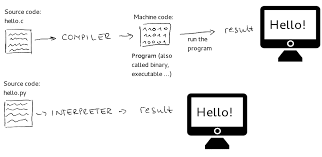
\includegraphics[width=0.7\linewidth]{index.png}
\caption{Interpreted vs compiled language}
\end{figure}

As a result, \(\tt{python}\) is essentially an \emph{interactive} programming language, you can program and see the results almost at the same time. This is very nice for a faster development since compilation time can be quite long (just to give an idea the compilation of our \texttt{C++} financial code takes more than one hour).
However there are drawbacks in terms of performance, the \emph{translation} to machine language has to be done in real-time resulting in slower execution times.

\begin{figure}[h]
\centering
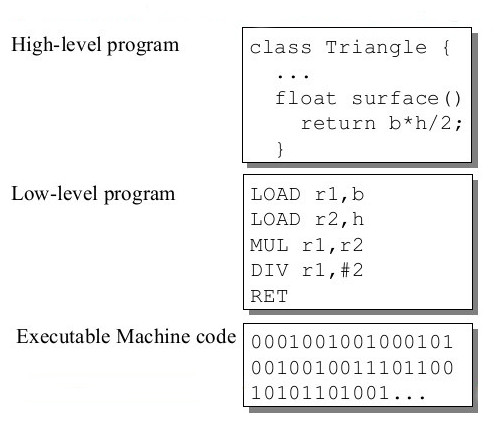
\includegraphics[width=0.5\linewidth]{machine_language.jpeg}
\caption{Human readable vs machine code}
\end{figure}

In the next chapters we'll take a quick tour of $\tt{python}$ and see the main features and characteristics of this programming language, later on we will see how it can be useful to solve real-world finance problems.

First of all since $\tt{python}$, as basically all programs, comes in different version and flavours we need to specify the particular one we are going to use.
The latest version (at the time I'm wrtiting this pages) is \(\tt{3.8.5}\), but it is continously evolving, however it is not difficult to see older versions floating around (e.g. \(\tt{2.7}\)).
This is because there are some big differences between \(\tt{python 2.X}\) and \(\tt{python 3.X}\) which prevent a sizeable portion of \(\tt{python 2}\) users to stick with it (consider that moving to \(\tt{python 3}\) would require a large amount of work to adapt big projects).
In conclusion we will concentrate on \textbf{\(\tt{python 3.7}\)}.

\section{$\tt{Python}$ basics}\label{python-basics}

Every language has \emph{keywords}, these are reserved words that have a special meaning and tell the computer what to do. The first one we encounter is \(\tt{print}\): it prints to screen whatever is specified between the parenthesis.

\begin{tcolorbox}[breakable, size=fbox, boxrule=1pt, pad at break*=1mm, colback=cellbackground, colframe=cellborder]
\begin{Verbatim}[commandchars=\\\{\}]
\PY{n+nb}{print} \PY{p}{(}\PY{l+s+s2}{\PYZdq{}}\PY{l+s+s2}{Hello world !}\PY{l+s+s2}{\PYZdq{}}\PY{p}{)} 

Hello world !
\end{Verbatim}
\end{tcolorbox}

\begin{tcolorbox}[breakable, size=fbox, boxrule=1pt, pad at break*=1mm, colback=cellbackground, colframe=cellborder]
\begin{Verbatim}[commandchars=\\\{\}]
\PY{n+nb}{print} \PY{p}{(}\PY{l+s+s2}{\PYZdq{}}\PY{l+s+s2}{Welcome}\PY{l+s+s2}{\PYZdq{}}\PY{p}{)}
\PY{n+nb}{print} \PY{p}{(}\PY{l+s+s2}{\PYZdq{}}\PY{l+s+s2}{to}\PY{l+s+s2}{\PYZdq{}}\PY{p}{)}
\PY{n+nb}{print} \PY{p}{(}\PY{l+s+s2}{\PYZdq{}}\PY{l+s+s2}{everybody}\PY{l+s+s2}{\PYZdq{}}\PY{p}{)}

Welcome
to
everybody
\end{Verbatim}
\end{tcolorbox}

Good programming practice recommends to document the code you write (you will soon see that it is surprisingly easy to forget what you wanted to do in your code). In \(\tt{python}\) you can add comments to code starting a line with a hash character (\#).

\begin{tcolorbox}[breakable, size=fbox, boxrule=1pt, pad at break*=1mm, colback=cellbackground, colframe=cellborder]
\begin{Verbatim}[commandchars=\\\{\}]
\PY{n+nb}{print} \PY{p}{(}\PY{l+s+s2}{\PYZdq{}}\PY{l+s+s2}{Ciao}\PY{l+s+s2}{\PYZdq{}}\PY{p}{)} \PY{c+c1}{\PYZsh{} this is a comment}

Ciao
\end{Verbatim}
\end{tcolorbox}

\subsection{Variables}\label{variables}

A variable is a computer memory location paired with an associated symbolic name, which contains some quantity of information referred to as a *value* (e.g.~a number, a string\ldots{}). Variables and hence data they contain, can be used, referenced and manipulated throughout a program.
A value is assigned to a variable with the equal operator (=). 

\begin{figure}[h]
\centering
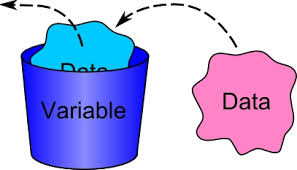
\includegraphics[width=0.5\linewidth]{var1.jpeg}
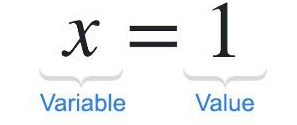
\includegraphics[width=0.5\linewidth]{var2.jpeg}
\caption{Graphical representation of a variable.}
\end{figure}

\begin{tcolorbox}[breakable, size=fbox, boxrule=1pt, pad at break*=1mm, colback=cellbackground, colframe=cellborder]
\begin{Verbatim}[commandchars=\\\{\}]
\PY{n}{x} \PY{o}{=} \PY{l+m+mi}{9}
\PY{n+nb}{print} \PY{p}{(}\PY{n}{x}\PY{p}{)}

9
\end{Verbatim}
\end{tcolorbox}

\begin{tcolorbox}[breakable, size=fbox, boxrule=1pt, pad at break*=1mm, colback=cellbackground, colframe=cellborder]
\begin{Verbatim}[commandchars=\\\{\}]
\PY{n}{myphone} \PY{o}{=} \PY{l+s+s2}{\PYZdq{}}\PY{l+s+s2}{Huawei P10Lite}\PY{l+s+s2}{\PYZdq{}}
\PY{n+nb}{print} \PY{p}{(}\PY{n}{myphone}\PY{p}{)}

Huawei P10Lite
\end{Verbatim}
\end{tcolorbox}

Another very useful keyword is \(\tt{type}\): it tells which kind of object is stored in a variable.

\begin{tcolorbox}[breakable, size=fbox, boxrule=1pt, pad at break*=1mm, colback=cellbackground, colframe=cellborder]
\begin{Verbatim}[commandchars=\\\{\}]
\PY{n+nb}{print} \PY{p}{(}\PY{n+nb}{type}\PY{p}{(}\PY{n}{x}\PY{p}{)}\PY{p}{)}
\PY{n+nb}{print} \PY{p}{(}\PY{n+nb}{type}\PY{p}{(}\PY{n}{myphone}\PY{p}{)}\PY{p}{)}

<class 'int'>
<class 'str'>
\end{Verbatim}
\end{tcolorbox}

After their definitions \(\tt{x}\) and \(\tt{myphone}\) can be used as aliases for a number and a string and their content manipulated, for example:

\begin{tcolorbox}[breakable, size=fbox, boxrule=1pt, pad at break*=1mm, colback=cellbackground, colframe=cellborder]
\begin{Verbatim}[commandchars=\\\{\}]
\PY{n+nb}{print} \PY{p}{(}\PY{n}{x}\PY{o}{+}\PY{l+m+mi}{5}\PY{p}{)}

14
\end{Verbatim}
\end{tcolorbox}

There are rules that limit the variable naming possibilities, in particular they must:
\begin{itemize}
\item begin with a letter (\tt{myphone}) or underscore (\tt{\_myphone});
\item other characters can be letters, numbers or more \_;
\item variable names are case-sensitive so \tt{myphone} and \tt{myPhone} are two distinct variables;
\end{itemize}

\textbf{Keywords, as said, are reserved words and as such cannot be used as variable names (e.g.~\(\tt{print, type, for...}\))}.

To use \textbf{good} variable names (and make you programs clearer and easier to read) always choose meaningful names instead of short names (i.e. \(\tt{numberOfCakes}\) is much better than simply \(\tt{n}\)), try to be consistent with your conventions (e.g.~choose once and for all between \(\tt{number\_of\_cakes}\) or
\(\tt{numberofcakes}\) or \(\tt{numberOfCakes}\)), usually begin a variable name with underscore (\_) only for a special case (will see later when this is usually done).

\subsection{Boolean expressions}\label{boolean-expressions}

Boolean expressions evaluate to \(\tt{true}\) or \(\tt{false}\) only. This type
of expressions usually involve logical or comparison operators like \(\tt{or}\), \(\tt{and}\), \textgreater{} (greater than), \textless{} (less than)\ldots{}
The equal boolean operator symbol is a double = (==), to not be confused with the assignement operator single = (=), with the first we compare two variables, with the second we associate a value to a variable.

Let's see some example. The following expression answer the question is 1 equal to 2:

\begin{tcolorbox}[breakable, size=fbox, boxrule=1pt, pad at break*=1mm, colback=cellbackground, colframe=cellborder]
\begin{Verbatim}[commandchars=\\\{\}]
\PY{l+m+mi}{1} \PY{o}{==} \PY{l+m+mi}{2} 

False
\end{Verbatim}
\end{tcolorbox}

Here another example using the not equal operator (!=):

\begin{tcolorbox}[breakable, size=fbox, boxrule=1pt, pad at break*=1mm, colback=cellbackground, colframe=cellborder]
\begin{Verbatim}[commandchars=\\\{\}]

True
\end{Verbatim}
\end{tcolorbox}

\begin{tcolorbox}[breakable, size=fbox, boxrule=1pt, pad at break*=1mm, colback=cellbackground, colframe=cellborder]
\begin{Verbatim}[commandchars=\\\{\}]
\PY{l+m+mi}{2} \PY{o}{\PYZlt{}} \PY{l+m+mi}{2}

False
\end{Verbatim}
\end{tcolorbox}

\begin{tcolorbox}[breakable, size=fbox, boxrule=1pt, pad at break*=1mm, colback=cellbackground, colframe=cellborder]
\begin{Verbatim}[commandchars=\\\{\}]
\PY{l+m+mi}{2} \PY{o}{\PYZlt{}}\PY{o}{=} \PY{l+m+mi}{2}  \PY{c+c1}{\PYZsh{} in this case we allow the numbers to be equal too}

True
\end{Verbatim}
\end{tcolorbox}

\begin{tcolorbox}[breakable, size=fbox, boxrule=1pt, pad at break*=1mm, colback=cellbackground, colframe=cellborder]
\begin{Verbatim}[commandchars=\\\{\}]
\PY{n+nb}{print} \PY{p}{(}\PY{n}{x}\PY{p}{)}
\PY{l+m+mi}{15} \PY{o}{\PYZlt{}}\PY{o}{=} \PY{n}{x} \PY{o+ow}{and} \PY{n}{x} \PY{o}{\PYZlt{}}\PY{o}{=} \PY{l+m+mi}{20} \PY{c+c1}{\PYZsh{} this expression could also be written as 15 \PYZlt{}= x \PYZlt{}= 20}

11
False
\end{Verbatim}
\end{tcolorbox}

\begin{tcolorbox}[breakable, size=fbox, boxrule=1pt, pad at break*=1mm, colback=cellbackground, colframe=cellborder]            
\begin{Verbatim}[commandchars=\\\{\}]
\PY{l+m+mi}{15} \PY{o}{\PYZlt{}}\PY{o}{=} \PY{n}{x} \PY{o+ow}{or} \PY{n}{x} \PY{o}{\PYZlt{}}\PY{o}{=} \PY{l+m+mi}{20}

True
\end{Verbatim}
\end{tcolorbox}

\begin{tcolorbox}[breakable, size=fbox, boxrule=1pt, pad at break*=1mm, colback=cellbackground, colframe=cellborder]            
\begin{Verbatim}[commandchars=\\\{\}]
\PY{o+ow}{not} \PY{p}{(}\PY{n}{x} \PY{o}{\PYZgt{}} \PY{l+m+mi}{20}\PY{p}{)} \PY{c+c1}{\PYZsh{} the not keyword negates the following expression}

True
\end{Verbatim}
\end{tcolorbox}

\subsection{String expressions}\label{string-expressions}

A ``string'' is a sequence of characters (letters, digits, spaces, punctuation\ldots{}). There are many operations that can be performed on strings, like for example concatenate (with + operator), truncate, replace characters\ldots{}

\begin{tcolorbox}[breakable, size=fbox, boxrule=1pt, pad at break*=1mm, colback=cellbackground, colframe=cellborder]            
\begin{Verbatim}[commandchars=\\\{\}]
\PY{n}{mystring} \PY{o}{=} \PY{l+s+s2}{\PYZdq{}}\PY{l+s+s2}{some text with punctuation, spaces and digits 10}\PY{l+s+s2}{\PYZdq{}}
\PY{n}{mystring}\PY{o}{.}\PY{n}{replace}\PY{p}{(}\PY{l+s+s2}{\PYZdq{}}\PY{l+s+s2}{s}\PY{l+s+s2}{\PYZdq{}}\PY{p}{,} \PY{l+s+s2}{\PYZdq{}}\PY{l+s+s2}{z}\PY{l+s+s2}{\PYZdq{}}\PY{p}{)}

'zome text with punctuation, zpacez and digitz 10'
\end{Verbatim}
\end{tcolorbox}

\begin{tcolorbox}[breakable, size=fbox, boxrule=1pt, pad at break*=1mm, colback=cellbackground, colframe=cellborder]            
\begin{Verbatim}[commandchars=\\\{\}]
\PY{l+s+s2}{\PYZdq{}}\PY{l+s+s2}{abc}\PY{l+s+s2}{\PYZdq{}} \PY{o}{+} \PY{l+s+s2}{\PYZdq{}}\PY{l+s+s2}{def}\PY{l+s+s2}{\PYZdq{}} \PY{c+c1}{\PYZsh{} it is possible to concatenate strings with + }

'abcdef'
\end{Verbatim}
\end{tcolorbox}

\begin{tcolorbox}[breakable, size=fbox, boxrule=1pt, pad at break*=1mm, colback=cellbackground, colframe=cellborder]            
\begin{Verbatim}[commandchars=\\\{\}]
\PY{l+s+s2}{\PYZdq{}}\PY{l+s+s2}{The number }\PY{l+s+s2}{\PYZdq{}} \PY{o}{+} \PY{l+m+mi}{4} \PY{o}{+} \PY{l+s+s2}{\PYZdq{}}\PY{l+s+s2}{ is my favourite number}\PY{l+s+s2}{\PYZdq{}}
\PY{c+c1}{\PYZsh{} this causes an error since we are trying to concatenate a string }
\PY{c+c1}{\PYZsh{} with a number so two different kind of objects}

---------------------------------------------------------------------------

TypeError                                 Traceback (most recent call last)

<ipython-input-33-b9f65c5a45f7> in <module>()
----> 1 "The number " + 4 + " is my favourite number"
      2 \# this causes an error since we are trying to concatenate a string
      3 \# with a number so two different kind of objects

TypeError: can only concatenate str (not "int") to str
\end{Verbatim}
\end{tcolorbox}

To avoid this error is possible to \textbf{cast} an object to a different type which means to convert an object to a different type. In this case we can \emph{force} the number four to be represented as a string with the \(\tt{str()}\) function:

\begin{tcolorbox}[breakable, size=fbox, boxrule=1pt, pad at break*=1mm, colback=cellbackground, colframe=cellborder]            
\begin{Verbatim}[commandchars=\\\{\}]
\PY{l+s+s2}{\PYZdq{}}\PY{l+s+s2}{The number }\PY{l+s+s2}{\PYZdq{}} \PY{o}{+} \PY{n+nb}{str}\PY{p}{(}\PY{l+m+mi}{4}\PY{p}{)} \PY{o}{+} \PY{l+s+s2}{\PYZdq{}}\PY{l+s+s2}{ is my favourite number}\PY{l+s+s2}{\PYZdq{}}

'The number 4 is my favourite number'
\end{Verbatim}
\end{tcolorbox}

\begin{tcolorbox}[breakable, size=fbox, boxrule=1pt, pad at break*=1mm, colback=cellbackground, colframe=cellborder]            
\begin{Verbatim}[commandchars=\\\{\}]
\PY{n+nb}{print} \PY{p}{(}\PY{n+nb}{type}\PY{p}{(}\PY{l+m+mf}{3.4}\PY{p}{)}\PY{p}{)}
\PY{n+nb}{print} \PY{p}{(}\PY{n+nb}{type}\PY{p}{(}\PY{n+nb}{str}\PY{p}{(}\PY{l+m+mf}{3.4}\PY{p}{)}\PY{p}{)}\PY{p}{)}

<class 'float'>
<class 'str'>
\end{Verbatim}
\end{tcolorbox}

In this simple case everything worked fine but type casting is not always possible: for example a number can be converted to a string (e.g.~from the integer 4 to the actual symbol ``4'') but the opposite is not possible (e.g.~cannot convert the string ``matteo'' to a meaningful number). In this second case we can try to use the function \(\tt{int()}\) to convert a string to an integer.

\begin{tcolorbox}[breakable, size=fbox, boxrule=1pt, pad at break*=1mm, colback=cellbackground, colframe=cellborder]            
\begin{Verbatim}[commandchars=\\\{\}]
\PY{n+nb}{int}\PY{p}{(}\PY{l+s+s2}{\PYZdq{}}\PY{l+s+s2}{matteo}\PY{l+s+s2}{\PYZdq{}}\PY{p}{)}

---------------------------------------------------------------------------

ValueError                                Traceback (most recent call last)

<ipython-input-17-979283bb65e4> in <module>
----> 1 int("matteo")  

ValueError: invalid literal for int() with base 10: 'matteo'
\end{Verbatim}
\end{tcolorbox}

\begin{tcolorbox}[breakable, size=fbox, boxrule=1pt, pad at break*=1mm, colback=cellbackground, colframe=cellborder]            
\begin{Verbatim}[commandchars=\\\{\}]
\PY{n+nb}{int}\PY{p}{(}\PY{l+s+s2}{\PYZdq{}}\PY{l+s+s2}{4}\PY{l+s+s2}{\PYZdq{}}\PY{p}{)}

4
\end{Verbatim}
\end{tcolorbox}

\paragraph{Pretty string formatting: } in order to get prettier strings than those obtained just concatenating with the + operator, \(\tt{python}\) allows to format text using the following syntax ``text {} other text''.format(variable).
With this notation, each {} is mapped to the variables listed in the $\tt{format}$ statement, the optional characters inside the curly brackets can determine the resulting format, for example in the following code $\tt{:.1f}$ means that this variable is float number and that has to be printed with 1 digit only after the decimal separator. 

\begin{tcolorbox}[breakable, size=fbox, boxrule=1pt, pad at break*=1mm, colback=cellbackground, colframe=cellborder]            
\begin{Verbatim}[commandchars=\\\{\}]
\PY{l+s+s2}{\PYZdq{}}\PY{l+s+s2}{The speed of light is about }\PY{l+s+si}{\PYZob{}:.1f\PYZcb{}}\PY{l+s+s2}{ }\PY{l+s+si}{\PYZob{}\PYZcb{}}\PY{l+s+s2}{\PYZdq{}}\PY{o}{.}\PY{n}{format}\PY{p}{(}\PY{l+m+mf}{299792.458}\PY{p}{,} \PY{l+s+s2}{\PYZdq{}}\PY{l+s+s2}{km/s}\PY{l+s+s2}{\PYZdq{}}\PY{p}{)}

'The speed of light is about 299792.5 km/s'
\end{Verbatim}
\end{tcolorbox}

In addition $\tt{format}$ allows for 0-padding of numbers, left or right alignement of text columns and so on.

\subsection{Mathematical expressions}\label{mathematical-expressions}

Below few examples of the basic mathematical expressions available in $\tt{python}$.

\begin{tcolorbox}[breakable, size=fbox, boxrule=1pt, pad at break*=1mm, colback=cellbackground, colframe=cellborder]            
\begin{Verbatim}[commandchars=\\\{\}]
\PY{l+m+mi}{1} \PY{o}{+} \PY{l+m+mi}{2}

3
\end{Verbatim}
\end{tcolorbox}

\begin{tcolorbox}[breakable, size=fbox, boxrule=1pt, pad at break*=1mm, colback=cellbackground, colframe=cellborder]            
\begin{Verbatim}[commandchars=\\\{\}]
\PY{l+m+mi}{40} \PY{o}{\PYZhy{}} \PY{l+m+mi}{5}

35
\end{Verbatim}
\end{tcolorbox}

\begin{tcolorbox}[breakable, size=fbox, boxrule=1pt, pad at break*=1mm, colback=cellbackground, colframe=cellborder]            
\begin{Verbatim}[commandchars=\\\{\}]
\PY{n}{x} \PY{o}{*} \PY{l+m+mi}{20} \PY{c+c1}{\PYZsh{} remember that we set x equal to 9}

180
\end{Verbatim}
\end{tcolorbox}

\begin{tcolorbox}[breakable, size=fbox, boxrule=1pt, pad at break*=1mm, colback=cellbackground, colframe=cellborder]            
\begin{Verbatim}[commandchars=\\\{\}]
\PY{n}{x} \PY{o}{/} \PY{l+m+mi}{4}

2.25
\end{Verbatim}
\end{tcolorbox}

\begin{tcolorbox}[breakable, size=fbox, boxrule=1pt, pad at break*=1mm, colback=cellbackground, colframe=cellborder]            
\begin{Verbatim}[commandchars=\\\{\}]
\PY{n+nb}{print} \PY{p}{(}\PY{n+nb}{type}\PY{p}{(}\PY{l+m+mf}{2.25}\PY{p}{)}\PY{p}{)}

<class 'float'>
\end{Verbatim}
\end{tcolorbox}

\begin{tcolorbox}[breakable, size=fbox, boxrule=1pt, pad at break*=1mm, colback=cellbackground, colframe=cellborder]            
\begin{Verbatim}[commandchars=\\\{\}]
\PY{n}{x} \PY{o}{/}\PY{o}{/} \PY{l+m+mi}{4} \PY{c+c1}{\PYZsh{} interger division \PYZhy{} result will be truncated to the }
       \PY{c+c1}{\PYZsh{} corresponding integer (no rounding)}
       \PY{c+c1}{\PYZsh{} 11 / 3 = 3.666666 \PYZhy{}\PYZgt{} 11 // 3 = 3}

2
\end{Verbatim}
\end{tcolorbox}

\begin{tcolorbox}[breakable, size=fbox, boxrule=1pt, pad at break*=1mm, colback=cellbackground, colframe=cellborder]            
\begin{Verbatim}[commandchars=\\\{\}]
\PY{n}{y} \PY{o}{=} \PY{l+m+mi}{3}
\PY{n}{x} \PY{o}{*}\PY{o}{*} \PY{n}{y} \PY{c+c1}{\PYZsh{} x to the power of y}

729
\end{Verbatim}
\end{tcolorbox}

\begin{tcolorbox}[breakable, size=fbox, boxrule=1pt, pad at break*=1mm, colback=cellbackground, colframe=cellborder]            
\begin{Verbatim}[commandchars=\\\{\}]
\PY{l+m+mi}{3} \PY{o}{*} \PY{p}{(}\PY{n}{x} \PY{o}{+} \PY{n}{y}\PY{p}{)}

36
\end{Verbatim}
\end{tcolorbox}

As an example of variable manipulation let's try to increment \(\tt{x}\) by 1 and save the result again in \(\tt{x}\).

\begin{tcolorbox}[breakable, size=fbox, boxrule=1pt, pad at break*=1mm, colback=cellbackground, colframe=cellborder]            
\begin{Verbatim}[commandchars=\\\{\}]
\PY{n+nb}{print} \PY{p}{(}\PY{n}{x}\PY{p}{)}
\PY{n}{x} \PY{o}{=} \PY{n}{x} \PY{o}{+} \PY{l+m+mi}{1}
\PY{n+nb}{print} \PY{p}{(}\PY{n}{x}\PY{p}{)}

15
16
\end{Verbatim}
\end{tcolorbox}

Sometimes the increment of a variable plus the assignment to the same variable is written with a more compact syntax \texttt{x += 1} (this is also true for other operators e.g. \texttt{x *= 2}).

More complex mathematical functions are not directly available, let's see for example the logarithm:

\begin{tcolorbox}[breakable, size=fbox, boxrule=1pt, pad at break*=1mm, colback=cellbackground, colframe=cellborder]            
\begin{Verbatim}[commandchars=\\\{\}]
\PY{n}{log}\PY{p}{(}\PY{l+m+mi}{3}\PY{p}{)}

---------------------------------------------------------------------------

NameError                                 Traceback (most recent call last)

<ipython-input-17-ffde4d60496a> in <module>()
    ----> 1 log(3) \# causes an error because the logarithm function
          2        \# is not available by default


NameError: name 'log' is not defined
\end{Verbatim}
\end{tcolorbox}

\section{Modules}\label{modules}

One very important feature of each language is the ability to reuse code among different programs, e.g.~imagine how awful would be if you had to reimplement every time you need it a function to compute the logarithm.
Usually there are mechanisms that allow to collect useful routines in \emph{packages} (or \emph{libraries}, or \emph{modules}) so that later they can be called and used by any program may need them.

These collections of utilities in \(\tt{python}\) are called \emph{modules} and each installation of this language brings with it a standard set of them. If you need more functionality, you can download more modules from the web (there are zillions out there) or if you are not satisfied with what you found you can write your own (which is one the goal of this course in the end).

Some examples of useful modules we will use are:

\begin{itemize}
\tightlist
\item
  Numpy - which provides matrix algebra functionality and much more;
\item
  Scipy - which provides a whole series of scientific computing
  functions;
\item
  Pandas - which provides tools for manipulating time series or dataset
  in general;
\item
  Matplotlib - for plotting graphs;
\item
  Jupyter - for notebooks like this one.
\end{itemize}

\begin{figure}
\centering
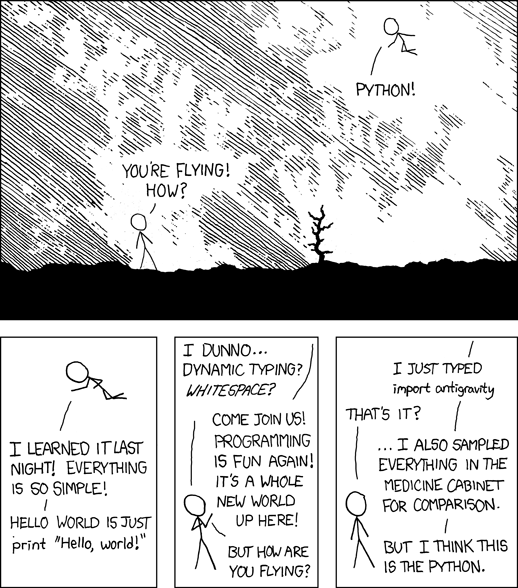
\includegraphics[width=0.75\linewidth]{python.png}
\caption{$\tt{Python}$ has many modules for download on the web\ldots{}}
\end{figure}

Later we will take a closer look at three modules which are quite useful in financial analysis.

In order to load a module in a \(\tt{python}\) program you can use the \(\tt{import}\) keyword. To inspect a module (to understand which are its functionalities) it can be used the \(\tt{help}\) and \(\tt{dir}\) keywords: the first write a help message which usually describes the functionalities of a module, the latter list all the available functions of a module.
\textbf{In order to access a function of a module you have to use the . (dot) operator: module-name.function-name.}

Let's see an example dealing with the\(\tt{math}\) module which implements the most common mathematical functions.

\begin{tcolorbox}[breakable, size=fbox, boxrule=1pt, pad at break*=1mm, colback=cellbackground, colframe=cellborder]            
\begin{Verbatim}[commandchars=\\\{\}]
\PY{k+kn}{import} \PY{n+nn}{math}
\PY{n+nb}{dir}\PY{p}{(}\PY{n}{math}\PY{p}{)}

{\color{outcolor}Out[{\color{outcolor}18}]:} ['\_\_doc\_\_',
          '\_\_loader\_\_',
          '\_\_name\_\_',
          '\_\_package\_\_',
          '\_\_spec\_\_',
          'acos',
          'acosh',
          'asin',
          'asinh',
          'atan',
          'atan2',
          'atanh',
          'ceil',
          'copysign',
          'cos',
          'cosh',
...
\end{Verbatim}
\end{tcolorbox}

\begin{tcolorbox}[breakable, size=fbox, boxrule=1pt, pad at break*=1mm, colback=cellbackground, colframe=cellborder]            
\begin{Verbatim}[commandchars=\\\{\}]
\PY{n+nb}{help}\PY{p}{(}\PY{n}{math}\PY{p}{)}

Help on module math:

NAME
    math

MODULE REFERENCE
    https://docs.python.org/3.6/library/math

    The following documentation is automatically generated from the Python
    source files.  It may be incomplete, incorrect or include features that
    are considered implementation detail and may vary between Python
    implementations.  When in doubt, consult the module reference at the
    location listed above.

DESCRIPTION
    This module is always available.  It provides access to the
    mathematical functions defined by the C standard.

FUNCTIONS
    acos({\ldots})
        acos(x)

        Return the arc cosine (measured in radians) of x.
...
\end{Verbatim}
\end{tcolorbox}

\begin{tcolorbox}[breakable, size=fbox, boxrule=1pt, pad at break*=1mm, colback=cellbackground, colframe=cellborder]            
\begin{Verbatim}[commandchars=\\\{\}]
\PY{n}{math}\PY{o}{.}\PY{n}{log}\PY{p}{(}\PY{l+m+mi}{3}\PY{p}{)}

1.0986122886681098
\end{Verbatim}
\end{tcolorbox}

\begin{tcolorbox}[breakable, size=fbox, boxrule=1pt, pad at break*=1mm, colback=cellbackground, colframe=cellborder]            
\begin{Verbatim}[commandchars=\\\{\}]
\PY{n}{math}\PY{o}{.}\PY{n}{exp}\PY{p}{(}\PY{l+m+mi}{3}\PY{p}{)}

20.085536923187668
\end{Verbatim}
\end{tcolorbox}

\begin{tcolorbox}[breakable, size=fbox, boxrule=1pt, pad at break*=1mm, colback=cellbackground, colframe=cellborder]            
\begin{Verbatim}[commandchars=\\\{\}]
\PY{n+nb}{print} \PY{p}{(}\PY{n+nb}{type}\PY{p}{(}\PY{n}{math}\PY{o}{.}\PY{n}{log}\PY{p}{)}\PY{p}{)} \PY{c+c1}{\PYZsh{} yet another type: builtin function}
\PY{n+nb}{print} \PY{p}{(}\PY{n+nb}{type}\PY{p}{(}\PY{n}{math}\PY{o}{.}\PY{n}{log}\PY{p}{(}\PY{l+m+mi}{3}\PY{p}{)}\PY{p}{)}\PY{p}{)}

<class 'builtin\_function\_or\_method'>
<class 'float'>
\end{Verbatim}
\end{tcolorbox}

If we want to avoid to type ``math.'' every time we compute a logarithm or an exponential, we can just import the needed functions from a module using the following syntax:

\begin{tcolorbox}[breakable, size=fbox, boxrule=1pt, pad at break*=1mm, colback=cellbackground, colframe=cellborder]            
\begin{Verbatim}[commandchars=\\\{\}]
\PY{k+kn}{from} \PY{n+nn}{math} \PY{k}{import} \PY{n}{log}\PY{p}{,} \PY{n}{exp}
\PY{n+nb}{print} \PY{p}{(}\PY{n}{log}\PY{p}{(}\PY{l+m+mi}{3}\PY{p}{)}\PY{p}{)}
\PY{n+nb}{print} \PY{p}{(}\PY{n}{exp}\PY{p}{(}\PY{l+m+mi}{3}\PY{p}{)}\PY{p}{)}

1.0986122886681098
20.085536923187668
\end{Verbatim}
\end{tcolorbox}

As an example let's compute the interest rate \(r\) that produces a return \(R\) of 11000 Euro when investing 10000 Euro for 2 years:

\(R = N\mathrm{e}^{r\tau} \rightarrow r = \frac{1}{\tau} \mathrm{log}(\frac{R}{N})\)

\begin{tcolorbox}[breakable, size=fbox, boxrule=1pt, pad at break*=1mm, colback=cellbackground, colframe=cellborder]            
\begin{Verbatim}[commandchars=\\\{\}]
\PY{n}{rate} \PY{o}{=} \PY{p}{(}\PY{l+m+mi}{1}\PY{o}{/}\PY{l+m+mi}{2}\PY{p}{)}\PY{o}{*}\PY{n}{log}\PY{p}{(}\PY{l+m+mf}{11000}\PY{o}{/}\PY{l+m+mi}{10000}\PY{p}{)}
\PY{n+nb}{print} \PY{p}{(}\PY{n}{rate}\PY{p}{)}

0.04765508990216247
\end{Verbatim}
\end{tcolorbox}

\section{Indented blocks and the $\tt{if/else}$ statement}\label{indented-blocks-and-the-ttifelse-statement}

Unlike other languages which uses parenthesis to isolate blocks of code $\tt{python}$ uses indentation. A first example of this is given by $\tt{if/then}$ statements. Such commands allow to dynamically run different blocks of code based on certain conditions. For example in the following we print different statements according to the value of $\tt{x}$, note the that the block of code to be run according each condition is shifted (i.e.~indented) with respect to the rest of the
code:

\begin{tcolorbox}[breakable, size=fbox, boxrule=1pt, pad at break*=1mm, colback=cellbackground, colframe=cellborder]            
\begin{Verbatim}[commandchars=\\\{\}]
\PY{n+nb}{print} \PY{p}{(}\PY{n}{x}\PY{p}{)}
\PY{k}{if} \PY{n}{x} \PY{o}{==} \PY{l+m+mi}{1}\PY{p}{:} 
    \PY{n+nb}{print} \PY{p}{(}\PY{l+s+s2}{\PYZdq{}}\PY{l+s+s2}{This will not be printed}\PY{l+s+s2}{\PYZdq{}}\PY{p}{)} 
    \PY{c+c1}{\PYZsh{} the block of code that is run if the first condition is met is indented}
\PY{k}{elif} \PY{n}{x} \PY{o}{==} \PY{l+m+mi}{15}\PY{p}{:}
    \PY{n+nb}{print} \PY{p}{(}\PY{l+s+s2}{\PYZdq{}}\PY{l+s+s2}{This will not be printed either}\PY{l+s+s2}{\PYZdq{}}\PY{p}{)}
    \PY{c+c1}{\PYZsh{} again the block of code that is run here is indented}
    \PY{c+c1}{\PYZsh{} to be \PYZdq{}isolated\PYZdq{} by the rest }
\PY{k}{else}\PY{p}{:}
    \PY{n+nb}{print} \PY{p}{(}\PY{l+s+s2}{\PYZdq{}}\PY{l+s+s2}{This *will* be printed}\PY{l+s+s2}{\PYZdq{}}\PY{p}{)}

16
This *will* be printed
\end{Verbatim}
\end{tcolorbox}

If by mistake the indentation of a block is missing an error is raised:
\begin{tcolorbox}[breakable, size=fbox, boxrule=1pt, pad at break*=1mm, colback=cellbackground, colframe=cellborder]            
\begin{Verbatim}[commandchars=\\\{\}]
\PY{k}{if} \PY{n}{x} \PY{o}{==} \PY{l+m+mi}{1}\PY{p}{:} 
\PY{n+nb}{print} \PY{p}{(}\PY{l+s+s2}{\PYZdq{}}\PY{l+s+s2}{This will not be printed}\PY{l+s+s2}{\PYZdq{}}\PY{p}{)}
\PY{k}{elif} \PY{n}{x} \PY{o}{==} \PY{l+m+mi}{15}\PY{p}{:}
    \PY{n+nb}{print} \PY{p}{(}\PY{l+s+s2}{\PYZdq{}}\PY{l+s+s2}{This will not be printed either}\PY{l+s+s2}{\PYZdq{}}\PY{p}{)}
\PY{k}{else}\PY{p}{:}
    \PY{n+nb}{print} \PY{p}{(}\PY{l+s+s2}{\PYZdq{}}\PY{l+s+s2}{This *will* be printed}\PY{l+s+s2}{\PYZdq{}}\PY{p}{)}

File "<ipython-input-38-4535a45a6419>", line 3
  print ("This will not be printed")
    \^{}
IndentationError: expected an indented block
\end{Verbatim}
\end{tcolorbox}

Below another example:
\begin{tcolorbox}[breakable, size=fbox, boxrule=1pt, pad at break*=1mm, colback=cellbackground, colframe=cellborder]            
\begin{Verbatim}[commandchars=\\\{\}]
\PY{k}{if} \PY{n}{x} \PY{o}{!=} \PY{l+m+mi}{1}\PY{p}{:}
   \PY{n+nb}{print} \PY{p}{(}\PY{l+s+s2}{\PYZdq{}}\PY{l+s+s2}{x does not equal to 1}\PY{l+s+s2}{\PYZdq{}}\PY{p}{)}

x does not equal to 1
\end{Verbatim}
\end{tcolorbox}

Just for comparison this is the same code written in $\tt{C++}$:

\begin{Shaded}
\begin{Highlighting}[]
\ControlFlowTok{if}\NormalTok{ (x == }\DecValTok{1}\NormalTok{) \{}
\NormalTok{ print (}\StringTok{"This will not be printed"}\NormalTok{);}
\NormalTok{\}}
\ControlFlowTok{else} \ControlFlowTok{if}\NormalTok{ (x == }\DecValTok{15}\NormalTok{) \{}
\NormalTok{  print (}\StringTok{"This will not be printed either"}\NormalTok{);}
\NormalTok{\}}
\ControlFlowTok{else}\NormalTok{ \{}
\NormalTok{print (}\StringTok{"This *will* be printed"}\NormalTok{);}
\NormalTok{\}}
\end{Highlighting}
\end{Shaded}

N.B. Notice how indentation doesn't matter at all here since the blocks are enclosed and defined by the brackets.

\section{Loops}\label{loops}

Another very important feature of a language is the ability to repeatedly run the same block of code many times. These is called looping and in \(\tt{python}\) can be done with $\tt{for}$ or $\tt{while}$ keywords.

\subsection{for}\label{for}

In a $\tt{for}$ loop we specifiy the set (or interval) over which we want to loop and a variable will assume all the values in that set (or interval). For example let's assume we want to print all the numbers between 25 and 30 excluded (here the keyword $\tt{range}$ returns the list of integers between the specified limits, if the first limit is not specified 0 is assumed):

\begin{tcolorbox}[breakable, size=fbox, boxrule=1pt, pad at break*=1mm, colback=cellbackground, colframe=cellborder]            
\begin{Verbatim}[commandchars=\\\{\}]
\PY{k}{for} \PY{n}{i} \PY{o+ow}{in} \PY{n+nb}{range}\PY{p}{(}\PY{l+m+mi}{25}\PY{p}{,} \PY{l+m+mi}{30}\PY{p}{)}\PY{p}{:}
     \PY{n+nb}{print} \PY{p}{(}\PY{n}{i}\PY{p}{)}

25
26
27
28
29
\end{Verbatim}
\end{tcolorbox}

At each cycle of the loop the variable $\tt{i}$ takes one of the values between
25 and 31. With $\tt{range}$ it is also possible to specify the step, so that the loop can jump every 2 units or to go in descending order:

\begin{tcolorbox}[breakable, size=fbox, boxrule=1pt, pad at break*=1mm, colback=cellbackground, colframe=cellborder]            
\begin{Verbatim}[commandchars=\\\{\}]
\PY{k}{for} \PY{n}{i} \PY{o+ow}{in} \PY{n+nb}{range} \PY{p}{(}\PY{l+m+mi}{30}\PY{p}{,} \PY{l+m+mi}{25}\PY{p}{,} \PY{o}{\PYZhy{}}\PY{l+m+mi}{1}\PY{p}{)}\PY{p}{:}
    \PY{n+nb}{print} \PY{p}{(}\PY{n}{i}\PY{p}{)}

30
29
28
27
26
\end{Verbatim}
\end{tcolorbox}

If it is needed to skip values in the loop the $\tt{continue}$ keyword can be used; in the code below 5 is actually missing from the list in the printout since it has been skipped by the $\tt{continue}$:

\begin{tcolorbox}[breakable, size=fbox, boxrule=1pt, pad at break*=1mm, colback=cellbackground, colframe=cellborder]            
\begin{Verbatim}[commandchars=\\\{\}]
\PY{k}{for} \PY{n}{i} \PY{o+ow}{in} \PY{n+nb}{range}\PY{p}{(}\PY{l+m+mi}{10}\PY{p}{)}\PY{p}{:}
    \PY{k}{if} \PY{n}{i} \PY{o}{==} \PY{l+m+mi}{5}\PY{p}{:}
        \PY{k}{continue} 
    \PY{n+nb}{print} \PY{p}{(}\PY{n}{i}\PY{p}{)}

0
1
2
3
4
6
7
8
9
\end{Verbatim}
\end{tcolorbox}

Instead of using $\tt{range}$ it is possbile to specify directly the set of looping values:

\begin{tcolorbox}[breakable, size=fbox, boxrule=1pt, pad at break*=1mm, colback=cellbackground, colframe=cellborder]            

\begin{Verbatim}[commandchars=\\\{\}]
\PY{k}{for} \PY{n}{i} \PY{o+ow}{in} \PY{p}{(}\PY{l+m+mi}{4}\PY{p}{,} \PY{l+m+mi}{6}\PY{p}{,} \PY{l+m+mi}{10}\PY{p}{,} \PY{l+m+mi}{20}\PY{p}{)}\PY{p}{:} \PY{c+c1}{\PYZsh{} here we loop directly on a list of numbers}
   \PY{n+nb}{print} \PY{p}{(}\PY{n}{i}\PY{p}{)}

4
6
10
20
\end{Verbatim}
\end{tcolorbox}

Finally looping on a string actually means to loop on each single character:
 
\begin{tcolorbox}[breakable, size=fbox, boxrule=1pt, pad at break*=1mm, colback=cellbackground, colframe=cellborder]            
\begin{Verbatim}[commandchars=\\\{\}]
\PY{n}{phrase} \PY{o}{=} \PY{l+s+s1}{\PYZsq{}}\PY{l+s+s1}{how to loop over a string}\PY{l+s+s1}{\PYZsq{}}
\PY{k}{for} \PY{n}{c} \PY{o+ow}{in} \PY{n}{phrase}\PY{p}{:}
   \PY{n+nb}{print} \PY{p}{(}\PY{n}{c}\PY{p}{)}

h
o
w
 
t
o
 
l
o
o
p
 
o
v
e
r
 
a
 
s
t
r
i
n
g
\end{Verbatim}
\end{tcolorbox}

\subsection{while}\label{while}

In a $\tt{for}$ loop we go through all the elements of a list of objects, the \texttt{while} statement instead repeats the same block of code untill a condition is met.
The following block of code is run if \texttt{x} squared is less than 50, so we first set \texttt{x=1} and at each iteration we increment it by 1 untill the condition is \texttt{True} (8 squared is 64 which is greater than 50):

\begin{tcolorbox}[breakable, size=fbox, boxrule=1pt, pad at break*=1mm, colback=cellbackground, colframe=cellborder]            
\begin{Verbatim}[commandchars=\\\{\}]
\PY{n}{x} \PY{o}{=} \PY{l+m+mi}{1}
\PY{k}{while} \PY{n}{x} \PY{o}{*}\PY{o}{*} \PY{l+m+mi}{2} \PY{o}{\PYZlt{}} \PY{l+m+mi}{50}\PY{p}{:}
   \PY{n+nb}{print} \PY{p}{(}\PY{n}{x}\PY{p}{)}
   \PY{n}{x} \PY{o}{+}\PY{o}{=} \PY{l+m+mi}{1}

1
2
3
4
5
6
7
\end{Verbatim}
\end{tcolorbox}

It is possible to exit prematurely from a \texttt{while} loop using the $\tt{break}$ keyword. In this case the while-condition is simply \texttt{True} so the code would run forever unless we set an exit strategy.

\begin{tcolorbox}[breakable, size=fbox, boxrule=1pt, pad at break*=1mm, colback=cellbackground, colframe=cellborder]            
\begin{Verbatim}[commandchars=\\\{\}]
\PY{n}{x} \PY{o}{=} \PY{l+m+mi}{1}
\PY{k}{while} \PY{k+kc}{True}\PY{p}{:}
  \PY{k}{if} \PY{p}{(}\PY{n}{x} \PY{o}{*}\PY{o}{*} \PY{l+m+mi}{2} \PY{o}{\PYZgt{}} \PY{l+m+mi}{50}\PY{p}{)}\PY{p}{:} 
      \PY{k}{break}
  \PY{n+nb}{print} \PY{p}{(}\PY{n}{x}\PY{p}{)}
  \PY{n}{x} \PY{o}{+}\PY{o}{=} \PY{l+m+mi}{1} 

1
2
3
4
5
6
7
\end{Verbatim}
\end{tcolorbox}

\clearpage
\chapter{Data Containers}\label{introduction-to-python---lesson-1.5}

In this chapter the container types available in $\tt{python}$ are reviewed.

\section{Lists}\label{lists}

A list in $\tt{python}$ is a container that is a \emph{mutable}, ordered sequence of elements. Each element or value that is inside of a list is called an *item*. Each item can be accessed using square brackets notation (very important, list indexing is zero-based so the first element is the 0th). A list is considered mutable since you can add, remove or update the items in it. Ordered instead means that items are kept in the same order they have been added.
Lists can be created by enclosing in square brackets the comma-separated list of the items or using the $\tt{list()}$ operator.

\begin{tcolorbox}[breakable, size=fbox, boxrule=1pt, pad at break*=1mm, colback=cellbackground, colframe=cellborder]
\begin{Verbatim}[commandchars=\\\{\}]
\PY{n}{mylist} \PY{o}{=} \PY{p}{[}\PY{l+m+mi}{21}\PY{p}{,} \PY{l+m+mi}{32}\PY{p}{,} \PY{l+m+mi}{15}\PY{p}{]}
\PY{n+nb}{print}\PY{p}{(}\PY{n}{mylist}\PY{p}{)}
\PY{n+nb}{print} \PY{p}{(}\PY{n+nb}{type}\PY{p}{(}\PY{n}{mylist}\PY{p}{)}\PY{p}{)}

[21, 32, 15]
\end{Verbatim}
\end{tcolorbox}

\begin{tcolorbox}[breakable, size=fbox, boxrule=1pt, pad at break*=1mm, colback=cellbackground, colframe=cellborder]
\begin{Verbatim}[commandchars=\\\{\}]
\PY{n+nb}{print}\PY{p}{(}\PY{n}{mylist}\PY{p}{[}\PY{l+m+mi}{0}\PY{p}{]}\PY{p}{)}

21
\end{Verbatim}
\end{tcolorbox}

If you have a list of lists (i.e. a 2-dimensional list) you can use the square brackets multiple times to access the inner elements:
\begin{tcolorbox}[breakable, size=fbox, boxrule=1pt, pad at break*=1mm,colback=cellbackground, colframe=cellborder]
\begin{Verbatim}[commandchars=\\\{\}]                 
\PY{n}{alist} \PY{o}{=} \PY{p}{[}\PY{p}{[}\PY{l+m+mi}{1}\PY{p}{,}\PY{l+m+mi}{2}\PY{p}{]}\PY{p}{,} \PY{p}{[}\PY{l+m+mi}{3}\PY{p}{,}\PY{l+m+mi}{4}\PY{p}{]}\PY{p}{,} \PY{p}{[}\PY{l+m+mi}{5}\PY{p}{,}\PY{l+m+mi}{6}\PY{p}{]}\PY{p}{]}       
\PY{n+nb}{print} \PY{p}{(}\PY{n}{alist}\PY{p}{[}\PY{l+m+mi}{1}\PY{p}{]}\PY{p}{[}\PY{l+m+mi}{1}\PY{p}{]}\PY{p}{)} \PY{c+c1}{\PYZsh{} first [1] returns [3,4], second returns 4}                   
\end{Verbatim} 
\end{tcolorbox}  

The number of elements in a list is counted using the keyword \texttt{len()}:
\begin{tcolorbox}[breakable, size=fbox, boxrule=1pt, pad at break*=1mm, colback=cellbackground, colframe=cellborder]
\begin{Verbatim}[commandchars=\\\{\}]
\PY{n+nb}{print}\PY{p}{(}\PY{n+nb}{len}\PY{p}{(}\PY{n}{mylist}\PY{p}{)}\PY{p}{)}

3
\end{Verbatim}
\end{tcolorbox}

Looping on list items can be achieved in two ways: using directly the list or by index:

\begin{tcolorbox}[breakable, size=fbox, boxrule=1pt, pad at break*=1mm, colback=cellbackground, colframe=cellborder]
\begin{Verbatim}[commandchars=\\\{\}]
\PY{n+nb}{print} \PY{p}{(}\PY{l+s+s2}{\PYZdq{}}\PY{l+s+s2}{Loop using the list itself:}\PY{l+s+s2}{\PYZdq{}}\PY{p}{)}
\PY{k}{for} \PY{n}{i} \PY{o+ow}{in} \PY{n}{mylist}\PY{p}{:}
    \PY{n+nb}{print} \PY{p}{(}\PY{n}{i}\PY{p}{)}

\PY{n+nb}{print} \PY{p}{(}\PY{l+s+s2}{\PYZdq{}}\PY{l+s+s2}{Loop by index:}\PY{l+s+s2}{\PYZdq{}}\PY{p}{)}
\PY{k}{for} \PY{n}{i} \PY{o+ow}{in} \PY{n+nb}{range}\PY{p}{(}\PY{n+nb}{len}\PY{p}{(}\PY{n}{mylist}\PY{p}{)}\PY{p}{)}\PY{p}{:} \PY{c+c1}{\PYZsh{} len() returns the number of items in a list}
    \PY{n+nb}{print} \PY{p}{(}\PY{n}{mylist}\PY{p}{[}\PY{n}{i}\PY{p}{]}\PY{p}{)}

Loop using the list itself:
21
32
15

Loop by index:
21
32
15
\end{Verbatim}
\end{tcolorbox}

With the \texttt{enumerate} function is actually possible to do both at the same time since it returns two values, the index of the item and its value, so in the example below, \texttt{i} will take the item index values while \texttt{item} the item value itself:

\begin{tcolorbox}[breakable, size=fbox, boxrule=1pt, pad at break*=1mm, colback=cellbackground, colframe=cellborder]
\begin{Verbatim}[commandchars=\\\{\}]
\PY{k}{for} \PY{n}{i}\PY{p}{,} \PY{n}{item} \PY{o+ow}{in} \PY{n+nb}{enumerate}\PY{p}{(}\PY{n}{mylist}\PY{p}{)}\PY{p}{:}                        
    \PY{n+nb}{print} \PY{p}{(}\PY{n}{i}\PY{p}{,} \PY{n}{item}\PY{p}{)}

0 21
1 74
2 85
3 15
4 188
\end{Verbatim}
\end{tcolorbox}

Since a list is mutable we can dynamically change its items:

\begin{tcolorbox}[breakable, size=fbox, boxrule=1pt, pad at break*=1mm, colback=cellbackground, colframe=cellborder]
\begin{Verbatim}[commandchars=\\\{\}]
\PY{n}{mylist}\PY{p}{[}\PY{l+m+mi}{1}\PY{p}{]} \PY{o}{=} \PY{l+m+mi}{74} \PY{c+c1}{\PYZsh{} we can change list items since it\PYZsq{}s *mutable*}
\PY{n+nb}{print} \PY{p}{(}\PY{n}{mylist}\PY{p}{)}

[21, 74, 15]
\end{Verbatim}
\end{tcolorbox}

With \texttt{append} an item is added at the end, while with \texttt{insert} an item can be added in a specified position:

\begin{tcolorbox}[breakable, size=fbox, boxrule=1pt, pad at break*=1mm, colback=cellbackground, colframe=cellborder]
\begin{Verbatim}[commandchars=\\\{\}]
\PY{n}{mylist}\PY{o}{.}\PY{n}{append}\PY{p}{(}\PY{l+m+mi}{188}\PY{p}{)} \PY{c+c1}{\PYZsh{} append add an item at the end of the list}
\PY{n+nb}{print} \PY{p}{(}\PY{n}{mylist}\PY{p}{)}

[21, 74, 15, 188]
\end{Verbatim}
\end{tcolorbox}

To append multiple values at once to a list a loop can be used but \texttt{python} offers a single line way of doing it: \texttt{[i*2 for i in range(10)]}. This syntax is called \emph{list comprehension}.

\begin{tcolorbox}[breakable, size=fbox, boxrule=1pt, pad at break*=1mm, colback=cellbackground, colframe=cellborder]
\begin{Verbatim}[commandchars=\\\{\}]
\PY{n}{mylist}\PY{o}{.}\PY{n}{insert}\PY{p}{(}\PY{l+m+mi}{2}\PY{p}{,} \PY{l+m+mi}{85}\PY{p}{)} \PY{c+c1}{\PYZsh{} insert an item in the desired position }
                     \PY{c+c1}{\PYZsh{} (2 in this example)}
\PY{n+nb}{print} \PY{p}{(}\PY{n}{mylist}\PY{p}{)}

[21, 74, 85, 15, 188]
\end{Verbatim}
\end{tcolorbox}

Accessing items outside the list range gives an error:

\begin{tcolorbox}[breakable, size=fbox, boxrule=1pt, pad at break*=1mm, colback=cellbackground, colframe=cellborder]
\begin{Verbatim}[commandchars=\\\{\}]
\PY{n}{mylist}\PY{p}{[}\PY{l+m+mi}{10}\PY{p}{]} \PY{c+c1}{\PYZsh{} error ! it doesn\PYZsq{}t exists, the list has only 3 }
           \PY{c+c1}{\PYZsh{} elements, so the last is item 2}

---------------------------------------------------------------------------

IndexError                                Traceback (most recent call last)

<ipython-input-36-ed1e5e6c3e46> in <module>
----> 1 mylist[10] \# error ! it doesn't exists, the list has only 3
      2           \# elements, so the last is item 2

IndexError: list index out of range
\end{Verbatim}
\end{tcolorbox}

There are two more nice features of $\tt{python}$ indexing: negative
indices are like positive ones except that they starts from the last
element, and \emph{slicing} whcih allows to specify a range of indices.

\begin{tcolorbox}[breakable, size=fbox, boxrule=1pt, pad at break*=1mm, colback=cellbackground, colframe=cellborder]
\begin{Verbatim}[commandchars=\\\{\}]
\PY{n+nb}{print} \PY{p}{(}\PY{l+s+s2}{\PYZdq{}}\PY{l+s+s2}{negative index \PYZhy{}1 returns the last element:}\PY{l+s+s2}{\PYZdq{}}\PY{p}{,} \PY{n}{mylist}\PY{p}{[}\PY{o}{\PYZhy{}}\PY{l+m+mi}{1}\PY{p}{]}\PY{p}{)}
\PY{n+nb}{print} \PY{p}{(}\PY{l+s+s2}{\PYZdq{}}\PY{l+s+s2}{slice [1:3] returns items between the 1st and 2nd:}\PY{l+s+s2}{\PYZdq{}}\PY{p}{,} \PY{n}{mylist}\PY{p}{[}\PY{l+m+mi}{0}\PY{p}{:}\PY{l+m+mi}{3}\PY{p}{]}\PY{p}{)}
\PY{n+nb}{print} \PY{p}{(}\PY{l+s+s2}{\PYZdq{}}\PY{l+s+s2}{slice [:2] returns items between the 1st and 2nd:}\PY{l+s+s2}{\PYZdq{}}\PY{p}{,} \PY{n}{mylist}\PY{p}{[}\PY{p}{:}\PY{l+m+mi}{2}\PY{p}{]}\PY{p}{)}
\PY{n+nb}{print} \PY{p}{(}\PY{l+s+s2}{\PYZdq{}}\PY{l+s+s2}{slice [2:] returns items between the 2nd and the last:}\PY{l+s+s2}{\PYZdq{}}\PY{p}{,} \PY{n}{mylist}\PY{p}{[}\PY{l+m+mi}{2}\PY{p}{:}\PY{p}{]}\PY{p}{)}

negative index -1 returns the last element: 188
slice [1:3] returns items between the 1st and 2nd: [21, 74, 85]
slice [:2] returns items between the 1st and 2nd: [21, 74]
slice [2:] returns items between the 2nd and the last: [85, 15, 188]
\end{Verbatim}
\end{tcolorbox}

It is worth mentioning that a list doesn't have to be populated
with the same kind of objects (list indices are instead always
integers).

\begin{tcolorbox}[breakable, size=fbox, boxrule=1pt, pad at break*=1mm, colback=cellbackground, colframe=cellborder]
\begin{Verbatim}[commandchars=\\\{\}]
\PY{n}{mixedlist} \PY{o}{=} \PY{p}{[}\PY{l+m+mi}{1}\PY{p}{,} \PY{l+m+mi}{2}\PY{p}{,} \PY{l+s+s2}{\PYZdq{}}\PY{l+s+s2}{b}\PY{l+s+s2}{\PYZdq{}}\PY{p}{,} \PY{n}{math}\PY{o}{.}\PY{n}{sqrt}\PY{p}{]}
\PY{n+nb}{print} \PY{p}{(}\PY{n}{mixedlist}\PY{p}{)}

[1, 2, 'b', <built-in function sqrt>]
\end{Verbatim}
\end{tcolorbox}

\begin{tcolorbox}[breakable, size=fbox, boxrule=1pt, pad at break*=1mm, colback=cellbackground, colframe=cellborder]
\begin{Verbatim}[commandchars=\\\{\}]
\PY{n+nb}{print} \PY{p}{(}\PY{n}{mixedlist}\PY{p}{[}\PY{l+s+s1}{\PYZsq{}}\PY{l+s+s1}{k}\PY{l+s+s1}{\PYZsq{}}\PY{p}{]}\PY{p}{)}

---------------------------------------------------------------------------

TypeError                                 Traceback (most recent call last)

<ipython-input-72-aea4c7f9789e> in <module>()
----> 1 print (mixedlist['k'])
    
TypeError: list indices must be integers or slices, not str
\end{Verbatim}
\end{tcolorbox}

A complete list of the commands available for a list can be shown with the $\tt{dir}$ statement:

\begin{tcolorbox}[breakable, size=fbox, boxrule=1pt, pad at break*=1mm,colback=cellbackground, colframe=cellborder]
\begin{Verbatim}[commandchars=\\\{\}]
\PY{n+nb}{dir}\PY{p}{(}\PY{n+nb}{list}\PY{p}{)}

[...
 'append',
 'clear',
 'copy',
 'count',
 'extend',
 'index',
 'insert',
 'pop',
 'remove',
 'reverse',
 'sort']
\end{Verbatim}
\end{tcolorbox}

Their meaning is pretty clear, so for example $\tt{sort}$ re-order the items according to a custom criteria or $\tt{index(item)}$ return the index of the specified item.

\section{Dictionaries}\label{dictionaries}

A we have seen lists are ordered collections of element and as such we can say that map integers (the index of each item) to values (any kind of \texttt{python} object). \emph{Dictionaries} generalize such a concept being containers which map \emph{keys} (\textbf{almost} any kind of \texttt{python} object) to values (any kind of \texttt{python} object).
In this case since the keys are not anymore necessarily integers there is no particular ordering of the items of a dictionary.

In our previous section we had:

\[ 0~(\textrm{0th item}) \rightarrow 21\]
\[ 1~(\textrm{1st item}) \rightarrow 74\]
\[ 2~(\textrm{2nd item}) \rightarrow 85\] \[ ... \]

With a dictionary we can have something like this:

\["apple" (\textrm{key}) \rightarrow 4 \]
\["banana" (\textrm{key}) \rightarrow 5 \]

As we will see dictionaries are very flexible and will be very usefull to represent complex data structures.

Dictionaries can be created by enclosing in curly brackets the comma-separated list of key-value pairs (key and value are separated by a :), or using the $\tt{dict()}$ operator.
In lists we could access items by index, here we do it by key still using the square brackets. Trying to access not existing keys results in error, but we can check if a key exists with the \texttt{in} operator.
As before, if a dictionary contains other dictionaries or lists, the square brackets can be applied repeatedly to access the inner items.

\begin{tcolorbox}[breakable, size=fbox, boxrule=1pt, pad at break*=1mm, colback=cellbackground, colframe=cellborder]
\begin{Verbatim}[commandchars=\\\{\}]
\PY{n}{adict} \PY{o}{=} \PY{p}{\PYZob{}}\PY{l+s+s2}{\PYZdq{}}\PY{l+s+s2}{apple}\PY{l+s+s2}{\PYZdq{}}\PY{p}{:} \PY{l+m+mi}{4}\PY{p}{,} \PY{l+s+s2}{\PYZdq{}}\PY{l+s+s2}{banana}\PY{l+s+s2}{\PYZdq{}}\PY{p}{:} \PY{l+m+mi}{5}\PY{p}{\PYZcb{}}
\PY{n+nb}{print} \PY{p}{(}\PY{n}{adict}\PY{p}{[}\PY{l+s+s2}{\PYZdq{}}\PY{l+s+s2}{apple}\PY{l+s+s2}{\PYZdq{}}\PY{p}{]}\PY{p}{)}

4
\end{Verbatim}
\end{tcolorbox}

\begin{tcolorbox}[breakable, size=fbox, boxrule=1pt, pad at break*=1mm, colback=cellbackground, colframe=cellborder]
\begin{Verbatim}[commandchars=\\\{\}]
\PY{n}{adict}\PY{p}{[}\PY{l+s+s2}{\PYZdq{}}\PY{l+s+s2}{pear}\PY{l+s+s2}{\PYZdq{}}\PY{p}{]} \PY{c+c1}{\PYZsh{} error !}

---------------------------------------------------------------------------

KeyError                                  Traceback (most recent call last)

<ipython-input-41-9d051ebd10de> in <module>
----> 1 adict["pear"] \# error ! this key doesn't exists
    
KeyError: 'pear'
\end{Verbatim}
\end{tcolorbox}

\begin{tcolorbox}[breakable, size=fbox, boxrule=1pt, pad at break*=1mm, colback=cellbackground, colframe=cellborder]
\begin{Verbatim}[commandchars=\\\{\}]
\PY{l+s+s2}{\PYZdq{}}\PY{l+s+s2}{pear}\PY{l+s+s2}{\PYZdq{}} \PY{o+ow}{in} \PY{n}{adict} \PY{c+c1}{\PYZsh{} indeed}

False
\end{Verbatim}
\end{tcolorbox}

The items can be dynamically created or updated with the assignement \texttt{=} operator, while again \texttt{len()} returns the number of items in a dictionary.

\begin{tcolorbox}[breakable, size=fbox, boxrule=1pt, pad at break*=1mm, colback=cellbackground, colframe=cellborder]
\begin{Verbatim}[commandchars=\\\{\}]
\PY{n}{adict}\PY{p}{[}\PY{l+s+s2}{\PYZdq{}}\PY{l+s+s2}{banana}\PY{l+s+s2}{\PYZdq{}}\PY{p}{]} \PY{o}{=} \PY{l+m+mi}{2}
\PY{n}{adict}\PY{p}{[}\PY{l+s+s2}{\PYZdq{}}\PY{l+s+s2}{pear}\PY{l+s+s2}{\PYZdq{}}\PY{p}{]} \PY{o}{=} \PY{l+m+mi}{10}
\PY{n+nb}{print} \PY{p}{(}\PY{n+nb}{len}\PY{p}{(}\PY{n}{adict}\PY{p}{)}\PY{p}{)}
\PY{n+nb}{print} \PY{p}{(}\PY{n}{adict}\PY{p}{)}

3
\{'apple': 4, 'banana': 2, 'pear': 10\}
\end{Verbatim}
\end{tcolorbox}

Dictionaries can be made of more complicated types than simple string and integers:

\begin{tcolorbox}[breakable, size=fbox, boxrule=1pt, pad at break*=1mm, colback=cellbackground, colframe=cellborder]
\begin{Verbatim}[commandchars=\\\{\}]
\PY{n}{adict}\PY{p}{[}\PY{n}{math}\PY{o}{.}\PY{n}{log}\PY{p}{]} \PY{o}{=} \PY{n}{math}\PY{o}{.}\PY{n}{exp}
\end{Verbatim}
\end{tcolorbox}

Also dictionaries can be created with the \emph{comprehension} syntax: \texttt{{i:v for i, v in enumerate(["a", "b", "c"])}}.

Looping over dictionary items can be done by key, by value or by both: \texttt{.keys()} returns a list of keys, \texttt{.values()} returns a list of values and \texttt{.items()} a list of pairs key-value.

\begin{tcolorbox}[breakable, size=fbox, boxrule=1pt, pad at break*=1mm, colback=cellbackground, colframe=cellborder]
\begin{Verbatim}[commandchars=\\\{\}]
\PY{n+nb}{print} \PY{p}{(}\PY{l+s+s2}{\PYZdq{}}\PY{l+s+s2}{All keys: }\PY{l+s+s2}{\PYZdq{}}\PY{p}{,} \PY{n}{adict}\PY{o}{.}\PY{n}{keys}\PY{p}{(}\PY{p}{)}\PY{p}{)}
\PY{k}{for} \PY{n}{key} \PY{o+ow}{in} \PY{n}{adict}\PY{o}{.}\PY{n}{keys}\PY{p}{(}\PY{p}{)}\PY{p}{:}
    \PY{n+nb}{print} \PY{p}{(}\PY{n}{key}\PY{p}{)}

\PY{n+nb}{print} \PY{p}{(}\PY{p}{)}
\PY{n+nb}{print} \PY{p}{(}\PY{l+s+s2}{\PYZdq{}}\PY{l+s+s2}{All values: }\PY{l+s+s2}{\PYZdq{}}\PY{p}{,} \PY{n}{adict}\PY{o}{.}\PY{n}{values}\PY{p}{(}\PY{p}{)}\PY{p}{)}
\PY{k}{for} \PY{n}{value} \PY{o+ow}{in} \PY{n}{adict}\PY{o}{.}\PY{n}{values}\PY{p}{(}\PY{p}{)}\PY{p}{:}
    \PY{n+nb}{print} \PY{p}{(}\PY{n}{value}\PY{p}{)}

\PY{n+nb}{print}\PY{p}{(}\PY{p}{)}
\PY{n+nb}{print} \PY{p}{(}\PY{l+s+s2}{\PYZdq{}}\PY{l+s+s2}{All key\PYZhy{}value pairs: }\PY{l+s+s2}{\PYZdq{}}\PY{p}{,} \PY{n}{adict}\PY{o}{.}\PY{n}{items}\PY{p}{(}\PY{p}{)}\PY{p}{)}
\PY{k}{for} \PY{n}{key}\PY{p}{,} \PY{n}{value} \PY{o+ow}{in} \PY{n}{adict}\PY{o}{.}\PY{n}{items}\PY{p}{(}\PY{p}{)}\PY{p}{:}
    \PY{n+nb}{print} \PY{p}{(}\PY{n}{key}\PY{p}{,} \PY{n}{value}\PY{p}{)}

All keys:  dict\_keys(['apple', 'banana', 'pear', <built-in function log>])
apple
banana
pear
<built-in function log>

All values:  dict\_values([4, 2, 10, <built-in function exp>])
4
2
10
<built-in function exp>

All key-value pairs:  dict\_items([('apple', 4), ('banana', 2), ('pear', 10),
(<built-in function log>, <built-in function exp>)])
apple 4
banana 2
pear 10
<built-in function log> <built-in function exp>
\end{Verbatim}
\end{tcolorbox}

To merge two dictionaries the function \texttt{update()} can be used, while with \texttt{del} it is possible to remove a key-value pair.

\begin{tcolorbox}[breakable, size=fbox, boxrule=1pt, pad at break*=1mm, colback=cellbackground, colframe=cellborder]
\begin{Verbatim}[commandchars=\\\{\}]
\PY{k}{del} \PY{n}{adict}\PY{p}{[}\PY{n}{math}\PY{o}{.}\PY{n}{log}\PY{p}{]}
\PY{n}{seconddict} \PY{o}{=} \PY{p}{\PYZob{}}\PY{l+s+s2}{\PYZdq{}}\PY{l+s+s2}{watermelon}\PY{l+s+s2}{\PYZdq{}}\PY{p}{:} \PY{l+m+mi}{0}\PY{p}{,} \PY{l+s+s2}{\PYZdq{}}\PY{l+s+s2}{strawberry}\PY{l+s+s2}{\PYZdq{}}\PY{p}{:} \PY{l+m+mi}{1}\PY{p}{\PYZcb{}}
\PY{n}{adict}\PY{o}{.}\PY{n}{update}\PY{p}{(}\PY{n}{seconddict}\PY{p}{)}
\PY{n+nb}{print} \PY{p}{(}\PY{n}{adict}\PY{p}{)}

\{'apple': 4, 'banana': 2, 'pear': 10, 'watermelon': 0, 'strawberry': 1\}
\end{Verbatim}
\end{tcolorbox}

Again the complete list of dictionary functions can be shown with $\tt{dir}$:

\begin{tcolorbox}[breakable, size=fbox, boxrule=1pt, pad at break*=1mm,colback=cellbackground, colframe=cellborder]
\begin{Verbatim}[commandchars=\\\{\}]
\PY{n+nb}{dir}\PY{p}{(}\PY{n+nb}{dict}\PY{p}{)}

[...
 'clear',
 'copy',
 'fromkeys',
 'get',
 'items',
 'keys',
 'pop',
 'popitem',
 'setdefault',
 'update',
 'values']
\end{Verbatim}
\end{tcolorbox}

\section{Tuples}\label{tuples}

Tuples create a bit of confusion for beginners because they are very similar to lists but they have some subtle conceptual differences.
Nonetheless, tuples do appear when programming in $\tt{python}$ so it's important to know about them.

\begin{figure}
\centering
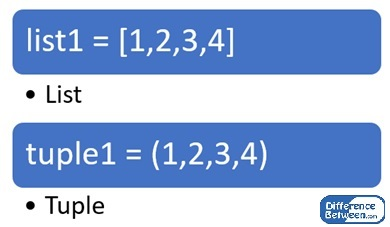
\includegraphics{Difference-Between-List-and-Tuple-fig-1-2.jpg}
\caption{At first glance list and tuples look very similar, but they are not\ldots{}}
\end{figure}

Like lists, tuples are containers of any type of object. Unlike lists though they are \emph{immutable} which means that once they have been created the content cannot be changed (i.e.~no append, insert or delete of the elements). Furthermore since they are immutable they can be used as dictionary keys (lists cannot).
To create a tuple the comma-separated list of items has to be enclosed in brackets, or the $\tt{tuple()}$ operator can be used.
Accessing tuple items is done in exactly the same way as lists.

\begin{tcolorbox}[breakable, size=fbox, boxrule=1pt, pad at break*=1mm, colback=cellbackground, colframe=cellborder]
\begin{Verbatim}[commandchars=\\\{\}]
\PY{n}{atuple} \PY{o}{=} \PY{p}{(}\PY{l+m+mi}{1}\PY{p}{,} \PY{l+m+mi}{2}\PY{p}{,} \PY{l+m+mi}{3}\PY{p}{)}
\PY{n+nb}{print} \PY{p}{(}\PY{l+s+s2}{\PYZdq{}}\PY{l+s+s2}{Length: }\PY{l+s+si}{\PYZob{}\PYZcb{}}\PY{l+s+s2}{\PYZdq{}}\PY{o}{.}\PY{n}{format}\PY{p}{(}\PY{n+nb}{len}\PY{p}{(}\PY{n}{atuple}\PY{p}{)}\PY{p}{)}\PY{p}{)}
\PY{n+nb}{print} \PY{p}{(}\PY{l+s+s2}{\PYZdq{}}\PY{l+s+s2}{First element: }\PY{l+s+si}{\PYZob{}\PYZcb{}}\PY{l+s+s2}{\PYZdq{}}\PY{o}{.}\PY{n}{format}\PY{p}{(}\PY{n}{atuple}\PY{p}{[}\PY{l+m+mi}{0}\PY{p}{]}\PY{p}{)}\PY{p}{)}
\PY{n+nb}{print} \PY{p}{(}\PY{l+s+s2}{\PYZdq{}}\PY{l+s+s2}{Last element: }\PY{l+s+si}{\PYZob{}\PYZcb{}}\PY{l+s+s2}{\PYZdq{}}\PY{o}{.}\PY{n}{format}\PY{p}{(}\PY{n}{atuple}\PY{p}{[}\PY{o}{\PYZhy{}}\PY{l+m+mi}{1}\PY{p}{]}\PY{p}{)}\PY{p}{)}

Length: 3
First element: 1
Last element: 3
\end{Verbatim}
\end{tcolorbox}

In the next snippet of code it is shown the so called unpacking which is another way to assign tuple values to variables.

\begin{tcolorbox}[breakable, size=fbox, boxrule=1pt, pad at break*=1mm, colback=cellbackground, colframe=cellborder]
\begin{Verbatim}[commandchars=\\\{\}]
\PY{n}{x}\PY{p}{,} \PY{n}{y}\PY{p}{,} \PY{n}{z} \PY{o}{=} \PY{p}{(}\PY{l+m+mi}{10}\PY{p}{,} \PY{l+m+mi}{5}\PY{p}{,} \PY{l+m+mi}{12}\PY{p}{)}
\PY{n+nb}{print} \PY{p}{(}\PY{l+s+s2}{\PYZdq{}}\PY{l+s+s2}{coord: x=}\PY{l+s+si}{\PYZob{}\PYZcb{}}\PY{l+s+s2}{ y=}\PY{l+s+si}{\PYZob{}\PYZcb{}}\PY{l+s+s2}{ z=}\PY{l+s+si}{\PYZob{}\PYZcb{}}\PY{l+s+s2}{\PYZdq{}}\PY{o}{.}\PY{n}{format}\PY{p}{(}\PY{n}{x}\PY{p}{,} \PY{n}{y}\PY{p}{,} \PY{n}{z}\PY{p}{)}\PY{p}{)}

coord: x=10 y=5 z=12
\end{Verbatim}
\end{tcolorbox}

If and ntuple has just one element don't forget the comma at the end otherwise it will be treated as a single number.

\begin{tcolorbox}[breakable, size=fbox, boxrule=1pt, pad at break*=1mm, colback=cellbackground, colframe=cellborder]
\begin{Verbatim}[commandchars=\\\{\}]
\PY{n}{tuple2} \PY{o}{=} \PY{p}{(}\PY{l+m+mi}{1}\PY{p}{,}\PY{p}{)}
\PY{n+nb}{print}\PY{p}{(}\PY{n+nb}{type}\PY{p}{(}\PY{n}{tuple2}\PY{p}{)}\PY{p}{)}
\PY{n}{tuple2} \PY{o}{=} \PY{p}{(}\PY{l+m+mi}{1}\PY{p}{)}
\PY{n+nb}{print}\PY{p}{(}\PY{n+nb}{type}\PY{p}{(}\PY{n}{tuple2}\PY{p}{)}\PY{p}{)}

<class 'tuple'>
<class 'int'>
\end{Verbatim}
\end{tcolorbox}

Since a tuple is immutable to add new elements it is necessary to create a new object:

\begin{tcolorbox}[breakable, size=fbox, boxrule=1pt, pad at break*=1mm, colback=cellbackground, colframe=cellborder]\begin{Verbatim}[commandchars=\\\{\}]
\PY{n}{tuple1} \PY{o}{=} \PY{p}{(}\PY{l+m+mi}{1}\PY{p}{,} \PY{l+m+mi}{2}\PY{p}{,} \PY{l+m+mi}{3}\PY{p}{)}
\PY{n}{tuple2} \PY{o}{=} \PY{n}{tuple1} \PY{o}{+} \PY{p}{(}\PY{l+m+mi}{4}\PY{p}{,} \PY{l+m+mi}{5}\PY{p}{)}
\PY{n+nb}{print}\PY{p}{(}\PY{n}{tuple2}\PY{p}{)}

(1,2,3,4,5)
\end{Verbatim}
\end{tcolorbox}

Finally, as already said tuples can be used as dictionary keys:

\begin{tcolorbox}[breakable, size=fbox, boxrule=1pt, pad at break*=1mm, colback=cellbackground, colframe=cellborder]\begin{Verbatim}[commandchars=\\\{\}]
\PY{n}{d} \PY{o}{=} \PY{p}{\PYZob{}}
   \PY{p}{(}\PY{l+s+s1}{\PYZsq{}}\PY{l+s+s1}{Finance}\PY{l+s+s1}{\PYZsq{}}\PY{p}{,} \PY{l+m+mi}{1}\PY{p}{)}\PY{p}{:} \PY{l+s+s1}{\PYZsq{}}\PY{l+s+s1}{Room 8}\PY{l+s+s1}{\PYZsq{}}\PY{p}{,}
    \PY{p}{(}\PY{l+s+s1}{\PYZsq{}}\PY{l+s+s1}{Finance}\PY{l+s+s1}{\PYZsq{}}\PY{p}{,} \PY{l+m+mi}{2}\PY{p}{)}\PY{p}{:} \PY{l+s+s1}{\PYZsq{}}\PY{l+s+s1}{Room 3}\PY{l+s+s1}{\PYZsq{}}\PY{p}{,}
    \PY{p}{(}\PY{l+s+s1}{\PYZsq{}}\PY{l+s+s1}{Math}\PY{l+s+s1}{\PYZsq{}}\PY{p}{,} \PY{l+m+mi}{1}\PY{p}{)}\PY{p}{:} \PY{l+s+s1}{\PYZsq{}}\PY{l+s+s1}{Room 6}\PY{l+s+s1}{\PYZsq{}}\PY{p}{,}
    \PY{p}{(}\PY{l+s+s1}{\PYZsq{}}\PY{l+s+s1}{Programming}\PY{l+s+s1}{\PYZsq{}}\PY{p}{,} \PY{l+m+mi}{1}\PY{p}{)}\PY{p}{:} \PY{l+s+s1}{\PYZsq{}}\PY{l+s+s1}{IT room}\PY{l+s+s1}{\PYZsq{}}
    \PY{p}{\PYZcb{}}
\end{Verbatim}
\end{tcolorbox}

Below the full list of tuple functions:
\begin{tcolorbox}[breakable, size=fbox, boxrule=1pt, pad at break*=1mm,colback=cellbackground, colframe=cellborder]
\begin{Verbatim}[commandchars=\\\{\}]
\PY{n+nb}{dir}\PY{p}{(}\PY{n+nb}{dict}\PY{p}{)}

[...
 'count',
 'index']
\end{Verbatim}
\end{tcolorbox}

\clearpage
\chapter{Date and Time}\label{introduction-to-python---lesson-1.6}

In this chapter we will take a little break and concentrate on a topic that it is not usually covered in this type of courses. However given its importance for financial computation the next paragraphs will be devoted to a close look up on the $\tt{datetime}$ module, whose utilities help in manipulating dates.

\section{Dates}\label{dates}

As said dates are not usually included in a standard \texttt{python} tutorial, however since they are pretty essential for finance we are going to cover this topic in some detail. In \texttt{python} the standard date class lives in the \texttt{datetime} module. We are also going to import \texttt{relativedelta} from the \texttt{dateutil} module, which allows to add/subtract days/months/years to dates, in other words to make operations on them.

In this first example the today's date is defined and with $\tt{relativedelta}$ two more date are created adding two months and three days to today.

\begin{tcolorbox}[breakable, size=fbox, boxrule=1pt, pad at break*=1mm,colback=cellbackground, colframe=cellborder]
\begin{Verbatim}[commandchars=\\\{\}]
\PY{k+kn}{from} \PY{n+nn}{datetime} \PY{k}{import} \PY{n}{date}\PY{p}{,} \PY{n}{datetime}
\PY{k+kn}{from} \PY{n+nn}{dateutil}\PY{n+nn}{.}\PY{n+nn}{relativedelta} \PY{k}{import} \PY{n}{relativedelta}

\PY{n}{date1} \PY{o}{=} \PY{n}{date}\PY{o}{.}\PY{n}{today}\PY{p}{(}\PY{p}{)}
\PY{n+nb}{print} \PY{p}{(}\PY{n}{date1}\PY{p}{)}
\PY{n}{date2} \PY{o}{=} \PY{n}{date}\PY{o}{.}\PY{n}{today}\PY{p}{(}\PY{p}{)} \PY{o}{+} \PY{n}{relativedelta}\PY{p}{(}\PY{n}{months}\PY{o}{=}\PY{l+m+mi}{2}\PY{p}{)}
\PY{n+nb}{print} \PY{p}{(}\PY{n}{date2}\PY{p}{)}
\PY{n}{date3} \PY{o}{=} \PY{n}{date}\PY{o}{.}\PY{n}{today}\PY{p}{(}\PY{p}{)} \PY{o}{\PYZhy{}} \PY{n}{relativedelta}\PY{p}{(}\PY{n}{days}\PY{o}{=}\PY{l+m+mi}{3}\PY{p}{)}
\PY{n+nb}{print} \PY{p}{(}\PY{n}{date3}\PY{p}{)}

2020-08-03
2020-10-03
2020-07-31
\end{Verbatim}
\end{tcolorbox}

Here instead another way of computing a new date is shown: in particular a one day delta is stored in a variable and today's date is moved by three days multiplying the defined delta by three.

\begin{tcolorbox}[breakable, size=fbox, boxrule=1pt, pad at break*=1mm,colback=cellbackground, colframe=cellborder]
\begin{Verbatim}[commandchars=\\\{\}]
\PY{n}{one\PYZus{}day} \PY{o}{=} \PY{n}{relativedelta}\PY{p}{(}\PY{n}{days}\PY{o}{=}\PY{l+m+mi}{1}\PY{p}{)}
\PY{n}{date}\PY{o}{.}\PY{n}{today}\PY{p}{(}\PY{p}{)} \PY{o}{\PYZhy{}} \PY{l+m+mi}{3} \PY{o}{*} \PY{n}{one\PYZus{}day}

datetime.date(2020, 7, 31)
\end{Verbatim}
\end{tcolorbox}

Next given two dates their difference is computed (and expressed in days).

\begin{tcolorbox}[breakable, size=fbox, boxrule=1pt, pad at break*=1mm,colback=cellbackground, colframe=cellborder]
\begin{Verbatim}[commandchars=\\\{\}]
\PY{n}{date1} \PY{o}{=} \PY{n}{date}\PY{p}{(}\PY{l+m+mi}{2019}\PY{p}{,} \PY{l+m+mi}{7}\PY{p}{,} \PY{l+m+mi}{2}\PY{p}{)}
\PY{n}{date2} \PY{o}{=} \PY{n}{date}\PY{p}{(}\PY{l+m+mi}{2019}\PY{p}{,} \PY{l+m+mi}{8}\PY{p}{,} \PY{l+m+mi}{16}\PY{p}{)}
\PY{p}{(}\PY{n}{date2} \PY{o}{\PYZhy{}} \PY{n}{date1}\PY{p}{)}\PY{o}{.}\PY{n}{days}

45
\end{Verbatim}
\end{tcolorbox}

Dates can be converted to and from strings and a large variety of formats can be specified in this conversions. The format is determined by a string in which each character starting with \% represent an element of the date, e.g. \%Y year, \%d day, \%s seconds, etc...

Below dates to string convertion:

\begin{tcolorbox}[breakable, size=fbox, boxrule=1pt, pad at break*=1mm,colback=cellbackground, colframe=cellborder]
\begin{Verbatim}[commandchars=\\\{\}]
\PY{n}{date1} \PY{o}{=} \PY{n}{date}\PY{p}{(}\PY{l+m+mi}{2019}\PY{p}{,} \PY{l+m+mi}{7}\PY{p}{,} \PY{l+m+mi}{2}\PY{p}{)}
\PY{n}{date1}\PY{o}{.}\PY{n}{strftime}\PY{p}{(}\PY{l+s+s2}{\PYZdq{}}\PY{l+s+s2}{\PYZpc{}}\PY{l+s+s2}{Y\PYZhy{}}\PY{l+s+s2}{\PYZpc{}}\PY{l+s+s2}{b\PYZhy{}}\PY{l+s+si}{\PYZpc{}d}\PY{l+s+s2}{ (}\PY{l+s+si}{\PYZpc{}a}\PY{l+s+s2}{)}\PY{l+s+s2}{\PYZdq{}}\PY{p}{)} \PY{c+c1}{\PYZsh{} dates can formatted in many ways}
                                \PY{c+c1}{\PYZsh{} check the docs for more details}

'2019-Jul-02 (Tue)'
\end{Verbatim}
\end{tcolorbox}

And here, strings are converted to datetime object:

\begin{tcolorbox}[breakable, size=fbox, boxrule=1pt, pad at break*=1mm,colback=cellbackground, colframe=cellborder]
\begin{Verbatim}[commandchars=\\\{\}]
\PY{c+c1}{\PYZsh{} a string can be convered to dates too}
\PY{n}{datetime}\PY{o}{.}\PY{n}{strptime}\PY{p}{(}\PY{l+s+s1}{\PYZsq{}}\PY{l+s+s1}{25 Aug 2019}\PY{l+s+s1}{\PYZsq{}}\PY{p}{,} \PY{l+s+s2}{\PYZdq{}}\PY{l+s+si}{\PYZpc{}d}\PY{l+s+s2}{ }\PY{l+s+s2}{\PYZpc{}}\PY{l+s+s2}{b }\PY{l+s+s2}{\PYZpc{}}\PY{l+s+s2}{Y}\PY{l+s+s2}{\PYZdq{}}\PY{p}{)}\PY{o}{.}\PY{n}{date}\PY{p}{(}\PY{p}{)}

datetime.date(2019, 8, 25)
\end{Verbatim}
\end{tcolorbox}

Finally a last example showing how to get the week-day from a date:

\begin{tcolorbox}[breakable, size=fbox, boxrule=1pt, pad at break*=1mm,colback=cellbackground, colframe=cellborder]
\begin{Verbatim}[commandchars=\\\{\}]
\PY{n}{date1}\PY{o}{.}\PY{n}{weekday}\PY{p}{(}\PY{p}{)} \PY{c+c1}{\PYZsh{} 0 = monday, ..., 6 = sunday}

1
\end{Verbatim}
\end{tcolorbox}

\clearpage
\chapter{Data Containers}\label{introduction-to-python---lesson-1.5}

In this chapter the container types available in $\tt{python}$ are reviewed.

\section{Lists}\label{lists}

A list in $\tt{python}$ is a container that is a \emph{mutable}, ordered sequence of elements. Each element or value that is inside of a list is called an \emph{item}. Each item can be accessed using square brackets notation (very important, list indexing is zero-based so the first element has index 0 actually). A list is considered mutable since you can add, remove or update the items in it. Ordered instead means that items are kept in the same order they have been added.
Lists can be created by enclosing in square brackets the comma-separated list of the items or using the $\tt{list()}$ operator.

\begin{tcolorbox}[breakable, size=fbox, boxrule=1pt, pad at break*=1mm, colback=cellbackground, colframe=cellborder]
  \begin{Verbatim}[commandchars=\\\{\}]
\PY{n}{mylist} \PY{o}{=} \PY{n+nb}{list}\PY{p}{([}\PY{l+m+mi}{21}\PY{p}{,} \PY{l+m+mi}{32}\PY{p}{,} \PY{l+m+mi}{15}\PY{p}{])}
\PY{n}{mylist} \PY{o}{=} \PY{p}{[}\PY{l+m+mi}{21}\PY{p}{,} \PY{l+m+mi}{32}\PY{p}{,} \PY{l+m+mi}{15}\PY{p}{]}
\PY{n+nb}{print}\PY{p}{(}\PY{n}{mylist}\PY{p}{)}
\PY{n+nb}{print} \PY{p}{(}\PY{n+nb}{type}\PY{p}{(}\PY{n}{mylist}\PY{p}{)}\PY{p}{)}

[21, 32, 15]
<class 'list'>
\end{Verbatim}
\end{tcolorbox}

\begin{tcolorbox}[breakable, size=fbox, boxrule=1pt, pad at break*=1mm, colback=cellbackground, colframe=cellborder]
\begin{Verbatim}[commandchars=\\\{\}]
\PY{n+nb}{print}\PY{p}{(}\PY{n}{mylist}\PY{p}{[}\PY{l+m+mi}{0}\PY{p}{]}\PY{p}{)}

21
\end{Verbatim}
\end{tcolorbox}

If you have a list of lists (i.e. a 2-dimensional list) you can use the square brackets multiple times to access the inner elements:
\begin{tcolorbox}[breakable, size=fbox, boxrule=1pt, pad at break*=1mm,colback=cellbackground, colframe=cellborder]
\begin{Verbatim}[commandchars=\\\{\}]                 
\PY{n}{alist} \PY{o}{=} \PY{p}{[}\PY{p}{[}\PY{l+m+mi}{1}\PY{p}{,}\PY{l+m+mi}{2}\PY{p}{]}\PY{p}{,} \PY{p}{[}\PY{l+m+mi}{3}\PY{p}{,}\PY{l+m+mi}{4}\PY{p}{]}\PY{p}{,} \PY{p}{[}\PY{l+m+mi}{5}\PY{p}{,}\PY{l+m+mi}{6}\PY{p}{]}\PY{p}{]}       
\PY{n+nb}{print} \PY{p}{(}\PY{n}{alist}\PY{p}{[}\PY{l+m+mi}{1}\PY{p}{]}\PY{p}{[}\PY{l+m+mi}{1}\PY{p}{]}\PY{p}{)} \PY{c+c1}{\PYZsh{} first [1] returns [3,4], second returns 4}                   
\end{Verbatim} 
\end{tcolorbox}  

The number of elements in a list is counted using the keyword \texttt{len()}:
\begin{tcolorbox}[breakable, size=fbox, boxrule=1pt, pad at break*=1mm, colback=cellbackground, colframe=cellborder]
\begin{Verbatim}[commandchars=\\\{\}]
\PY{n+nb}{print}\PY{p}{(}\PY{n+nb}{len}\PY{p}{(}\PY{n}{mylist}\PY{p}{)}\PY{p}{)}

3
\end{Verbatim}
\end{tcolorbox}

Looping on list items can be achieved in two ways: using directly the list or by index:

\begin{tcolorbox}[breakable, size=fbox, boxrule=1pt, pad at break*=1mm, colback=cellbackground, colframe=cellborder]
\begin{Verbatim}[commandchars=\\\{\}]
\PY{n+nb}{print} \PY{p}{(}\PY{l+s+s2}{\PYZdq{}}\PY{l+s+s2}{Loop using the list itself:}\PY{l+s+s2}{\PYZdq{}}\PY{p}{)}
\PY{k}{for} \PY{n}{i} \PY{o+ow}{in} \PY{n}{mylist}\PY{p}{:}
    \PY{n+nb}{print} \PY{p}{(}\PY{n}{i}\PY{p}{)}

\PY{n+nb}{print} \PY{p}{(}\PY{l+s+s2}{\PYZdq{}}\PY{l+s+s2}{Loop by index:}\PY{l+s+s2}{\PYZdq{}}\PY{p}{)}
\PY{k}{for} \PY{n}{i} \PY{o+ow}{in} \PY{n+nb}{range}\PY{p}{(}\PY{n+nb}{len}\PY{p}{(}\PY{n}{mylist}\PY{p}{)}\PY{p}{)}\PY{p}{:} \PY{c+c1}{\PYZsh{} len() returns the number of items in a list}
    \PY{n+nb}{print} \PY{p}{(}\PY{n}{mylist}\PY{p}{[}\PY{n}{i}\PY{p}{]}\PY{p}{)}

Loop using the list itself:
21
32
15

Loop by index:
21
32
15
\end{Verbatim}
\end{tcolorbox}

With the \texttt{enumerate} function is actually possible to do both at the same time since it returns two values, the index of the item and its value, so in the example below, \texttt{i} will take the item index values while \texttt{item} the item value itself:

\begin{tcolorbox}[breakable, size=fbox, boxrule=1pt, pad at break*=1mm, colback=cellbackground, colframe=cellborder]
\begin{Verbatim}[commandchars=\\\{\}]
\PY{k}{for} \PY{n}{i}\PY{p}{,} \PY{n}{item} \PY{o+ow}{in} \PY{n+nb}{enumerate}\PY{p}{(}\PY{n}{mylist}\PY{p}{)}\PY{p}{:}                        
    \PY{n+nb}{print} \PY{p}{(}\PY{n}{i}\PY{p}{,} \PY{n}{item}\PY{p}{)}

0 21
1 74
2 85
3 15
4 188
\end{Verbatim}
\end{tcolorbox}

Since a list is mutable we can dynamically change its items:

\begin{tcolorbox}[breakable, size=fbox, boxrule=1pt, pad at break*=1mm, colback=cellbackground, colframe=cellborder]
\begin{Verbatim}[commandchars=\\\{\}]
\PY{n}{mylist}\PY{p}{[}\PY{l+m+mi}{1}\PY{p}{]} \PY{o}{=} \PY{l+m+mi}{74} \PY{c+c1}{\PYZsh{} we can change list items since it\PYZsq{}s *mutable*}
\PY{n+nb}{print} \PY{p}{(}\PY{n}{mylist}\PY{p}{)}

[21, 74, 15]
\end{Verbatim}
\end{tcolorbox}

With \texttt{append} an item is added at the end, while with \texttt{insert} an item can be added in a specified position:

\begin{tcolorbox}[breakable, size=fbox, boxrule=1pt, pad at break*=1mm, colback=cellbackground, colframe=cellborder]
\begin{Verbatim}[commandchars=\\\{\}]
\PY{n}{mylist}\PY{o}{.}\PY{n}{append}\PY{p}{(}\PY{l+m+mi}{188}\PY{p}{)} \PY{c+c1}{\PYZsh{} append add an item at the end of the list}
\PY{n+nb}{print} \PY{p}{(}\PY{n}{mylist}\PY{p}{)}

[21, 74, 15, 188]

\PY{n}{mylist}\PY{o}{.}\PY{n}{insert}\PY{p}{(}\PY{l+m+mi}{2}\PY{p}{,} \PY{l+m+mi}{85}\PY{p}{)} \PY{c+c1}{\PYZsh{} insert an item in the desired position }
                     \PY{c+c1}{\PYZsh{} (2 in this example)}
\PY{n+nb}{print} \PY{p}{(}\PY{n}{mylist}\PY{p}{)}

[21, 74, 85, 15, 188]
\end{Verbatim}
\end{tcolorbox}

To append multiple values at once to a list a loop can be used but \texttt{python} offers a single line way of doing it: \texttt{[i*2 for i in range(10)]}. This syntax is called \emph{list comprehension}.

Accessing items outside the list range gives an error:

\begin{tcolorbox}[breakable, size=fbox, boxrule=1pt, pad at break*=1mm, colback=cellbackground, colframe=cellborder]
\begin{Verbatim}[commandchars=\\\{\}]
\PY{n}{mylist}\PY{p}{[}\PY{l+m+mi}{10}\PY{p}{]} \PY{c+c1}{\PYZsh{} error ! it doesn\PYZsq{}t exists, the list has only 3 }
           \PY{c+c1}{\PYZsh{} elements, so the last is item 2}

---------------------------------------------------------------------------

IndexError                                Traceback (most recent call last)

<ipython-input-36-ed1e5e6c3e46> in <module>
----> 1 mylist[10] \# error ! it doesn't exists, the list has only 3
      2           \# elements, so the last is item 2

IndexError: list index out of range
\end{Verbatim}
\end{tcolorbox}

Read carefully the error messages usually they are very explicative and can help a lot in \emph{debugging} (i.e. finding mistakes) in your programs.

There are two more nice features of $\tt{python}$ indexing:

\begin{itemize}
\item negative indices are like positive ones except that they starts from the last element;
\item \emph{slicing} which allows to specify a range of indices to select more items at once (if the first or last limits are missing slicing will start from the first or end with last index respectively).
\end{itemize}

\begin{tcolorbox}[breakable, size=fbox, boxrule=1pt, pad at break*=1mm, colback=cellbackground, colframe=cellborder]
\begin{Verbatim}[commandchars=\\\{\}]
\PY{n+nb}{print} \PY{p}{(}\PY{l+s+s2}{\PYZdq{}}\PY{l+s+s2}{negative index \PYZhy{}1 returns the last element:}\PY{l+s+s2}{\PYZdq{}}\PY{p}{,} \PY{n}{mylist}\PY{p}{[}\PY{o}{\PYZhy{}}\PY{l+m+mi}{1}\PY{p}{]}\PY{p}{)}
\PY{n+nb}{print} \PY{p}{(}\PY{l+s+s2}{\PYZdq{}}\PY{l+s+s2}{slice [1:3] returns items 1st and 2nd:}\PY{l+s+s2}{\PYZdq{}}\PY{p}{,} \PY{n}{mylist}\PY{p}{[}\PY{l+m+mi}{0}\PY{p}{:}\PY{l+m+mi}{3}\PY{p}{]}\PY{p}{)}
\PY{n+nb}{print} \PY{p}{(}\PY{l+s+s2}{\PYZdq{}}\PY{l+s+s2}{slice [:2] returns items 0th and 1st:}\PY{l+s+s2}{\PYZdq{}}\PY{p}{,} \PY{n}{mylist}\PY{p}{[}\PY{p}{:}\PY{l+m+mi}{2}\PY{p}{]}\PY{p}{)}
\PY{n+nb}{print} \PY{p}{(}\PY{l+s+s2}{\PYZdq{}}\PY{l+s+s2}{slice [2:] returns items between the 2nd and the last:}\PY{l+s+s2}{\PYZdq{}}\PY{p}{,} \PY{n}{mylist}\PY{p}{[}\PY{l+m+mi}{2}\PY{p}{:}\PY{p}{]}\PY{p}{)}

negative index -1 returns the last element: 188
slice [1:3] returns items 1st and 2nd: [21, 74, 85]
slice [:2] returns items 0th and 1st: [21, 74]
slice [2:] returns items between the 2nd and the last: [85, 15, 188]
\end{Verbatim}
\end{tcolorbox}

Needless to say that slicing with \texttt{[:]} returns the entire list.

It is worth mentioning that a list doesn't have to be populated
with the same kind of objects (list indices are instead always
integers).

\begin{tcolorbox}[breakable, size=fbox, boxrule=1pt, pad at break*=1mm, colback=cellbackground, colframe=cellborder]
\begin{Verbatim}[commandchars=\\\{\}]
\PY{n}{mixedlist} \PY{o}{=} \PY{p}{[}\PY{l+m+mi}{1}\PY{p}{,} \PY{l+m+mi}{2}\PY{p}{,} \PY{l+s+s2}{\PYZdq{}}\PY{l+s+s2}{b}\PY{l+s+s2}{\PYZdq{}}\PY{p}{,} \PY{n}{math}\PY{o}{.}\PY{n}{sqrt}\PY{p}{]}
\PY{n+nb}{print} \PY{p}{(}\PY{n}{mixedlist}\PY{p}{)}

[1, 2, 'b', <built-in function sqrt>]
\end{Verbatim}
\end{tcolorbox}

\begin{tcolorbox}[breakable, size=fbox, boxrule=1pt, pad at break*=1mm, colback=cellbackground, colframe=cellborder]
\begin{Verbatim}[commandchars=\\\{\}]
\PY{n+nb}{print} \PY{p}{(}\PY{n}{mixedlist}\PY{p}{[}\PY{l+s+s1}{\PYZsq{}}\PY{l+s+s1}{k}\PY{l+s+s1}{\PYZsq{}}\PY{p}{]}\PY{p}{)}

---------------------------------------------------------------------------

TypeError                                 Traceback (most recent call last)

<ipython-input-72-aea4c7f9789e> in <module>()
----> 1 print (mixedlist['k'])
    
TypeError: list indices must be integers or slices, not str
\end{Verbatim}
\end{tcolorbox}

A complete list of the commands available for a list can be shown with the $\tt{dir}$ statement:

\begin{tcolorbox}[breakable, size=fbox, boxrule=1pt, pad at break*=1mm,colback=cellbackground, colframe=cellborder]
\begin{Verbatim}[commandchars=\\\{\}]
\PY{n+nb}{dir}\PY{p}{(}\PY{n+nb}{list}\PY{p}{)}

[...
 'append',
 'clear',
 'copy',
 'count',
 'extend',
 'index',
 'insert',
 'pop',
 'remove',
 'reverse',
 'sort']
\end{Verbatim}
\end{tcolorbox}

Their meaning is pretty clear, so for example $\tt{sort}$ re-order the items according to a custom criteria or $\tt{index(item)}$ return the index of the specified item.

\section{Dictionaries}\label{dictionaries}

A we have seen lists are ordered collections of elements and as such we can say that map integers (the index of each item) to values (any kind of \texttt{python} object). \emph{Dictionaries} generalize such a concept being containers which map \emph{keys} (\textbf{almost} any kind of \texttt{python} object) to values (any kind of \texttt{python} object).

In our previous section we had:

\[ 0~(\textrm{0th item}) \rightarrow 21\]
\[ 1~(\textrm{1st item}) \rightarrow 74\]
\[ 2~(\textrm{2nd item}) \rightarrow 85\] \[ ... \]

With a dictionary we can have something like this:

\["apple" (\textrm{key}) \rightarrow 4 \]
\["banana" (\textrm{key}) \rightarrow 5 \]

As we will see dictionaries are very flexible and will be very useful to represent complex data structures.

Dictionaries can be created by enclosing in curly brackets the comma-separated list of key-value pairs (key and value are separated by a :), or using the $\tt{dict()}$ operator.
In lists we could access items by index, here we do it by key still using the square brackets. Trying to access not existing keys results in error, but we can check if a key exists with the \texttt{in} operator.
As before, if a dictionary contains other dictionaries or lists, the square brackets can be applied repeatedly to access the inner items.

\begin{tcolorbox}[breakable, size=fbox, boxrule=1pt, pad at break*=1mm, colback=cellbackground, colframe=cellborder]
\begin{Verbatim}[commandchars=\\\{\}]
\PY{n}{adict} \PY{o}{=} \PY{p}{\PYZob{}}\PY{l+s+s2}{\PYZdq{}}\PY{l+s+s2}{apple}\PY{l+s+s2}{\PYZdq{}}\PY{p}{:} \PY{l+m+mi}{4}\PY{p}{,} \PY{l+s+s2}{\PYZdq{}}\PY{l+s+s2}{banana}\PY{l+s+s2}{\PYZdq{}}\PY{p}{:} \PY{l+m+mi}{5}\PY{p}{\PYZcb{}}
\PY{n+nb}{print} \PY{p}{(}\PY{n}{adict}\PY{p}{[}\PY{l+s+s2}{\PYZdq{}}\PY{l+s+s2}{apple}\PY{l+s+s2}{\PYZdq{}}\PY{p}{]}\PY{p}{)}

4
\end{Verbatim}
\end{tcolorbox}

\begin{tcolorbox}[breakable, size=fbox, boxrule=1pt, pad at break*=1mm, colback=cellbackground, colframe=cellborder]
\begin{Verbatim}[commandchars=\\\{\}]
\PY{n}{adict}\PY{p}{[}\PY{l+s+s2}{\PYZdq{}}\PY{l+s+s2}{pear}\PY{l+s+s2}{\PYZdq{}}\PY{p}{]} \PY{c+c1}{\PYZsh{} error !}

---------------------------------------------------------------------------

KeyError                                  Traceback (most recent call last)

<ipython-input-41-9d051ebd10de> in <module>
----> 1 adict["pear"] \# error ! this key doesn't exists
    
KeyError: 'pear'
\end{Verbatim}
\end{tcolorbox}

\begin{tcolorbox}[breakable, size=fbox, boxrule=1pt, pad at break*=1mm, colback=cellbackground, colframe=cellborder]
\begin{Verbatim}[commandchars=\\\{\}]
\PY{l+s+s2}{\PYZdq{}}\PY{l+s+s2}{pear}\PY{l+s+s2}{\PYZdq{}} \PY{o+ow}{in} \PY{n}{adict} \PY{c+c1}{\PYZsh{} indeed}

False
\end{Verbatim}
\end{tcolorbox}

The items can be dynamically created or updated with the assignment \texttt{=} operator, while again \texttt{len()} returns the number of items in a dictionary.

\begin{tcolorbox}[breakable, size=fbox, boxrule=1pt, pad at break*=1mm, colback=cellbackground, colframe=cellborder]
\begin{Verbatim}[commandchars=\\\{\}]
\PY{n}{adict}\PY{p}{[}\PY{l+s+s2}{\PYZdq{}}\PY{l+s+s2}{banana}\PY{l+s+s2}{\PYZdq{}}\PY{p}{]} \PY{o}{=} \PY{l+m+mi}{2}
\PY{n}{adict}\PY{p}{[}\PY{l+s+s2}{\PYZdq{}}\PY{l+s+s2}{pear}\PY{l+s+s2}{\PYZdq{}}\PY{p}{]} \PY{o}{=} \PY{l+m+mi}{10}
\PY{n+nb}{print} \PY{p}{(}\PY{n+nb}{len}\PY{p}{(}\PY{n}{adict}\PY{p}{)}\PY{p}{)}
\PY{n+nb}{print} \PY{p}{(}\PY{n}{adict}\PY{p}{)}

3
\{'apple': 4, 'banana': 2, 'pear': 10\}
\end{Verbatim}
\end{tcolorbox}

Dictionaries can be made of more complicated types than simple string and integers:

\begin{tcolorbox}[breakable, size=fbox, boxrule=1pt, pad at break*=1mm, colback=cellbackground, colframe=cellborder]
\begin{Verbatim}[commandchars=\\\{\}]
\PY{n}{adict}\PY{p}{[}\PY{n}{math}\PY{o}{.}\PY{n}{log}\PY{p}{]} \PY{o}{=} \PY{n}{math}\PY{o}{.}\PY{n}{exp}
\end{Verbatim}
\end{tcolorbox}

Also dictionaries can be created with the \emph{comprehension} syntax: \texttt{\{i:v for i, v in enumerate(["a", "b", "c"])\}}.

Looping over dictionary items can be done by key, by value or by both: \texttt{.keys()} returns a list of keys, \texttt{.values()} returns a list of values and \texttt{.items()} a list of pairs key-value.

\begin{tcolorbox}[breakable, size=fbox, boxrule=1pt, pad at break*=1mm, colback=cellbackground, colframe=cellborder]
\begin{Verbatim}[commandchars=\\\{\}]
\PY{n+nb}{print} \PY{p}{(}\PY{l+s+s2}{\PYZdq{}}\PY{l+s+s2}{All keys: }\PY{l+s+s2}{\PYZdq{}}\PY{p}{,} \PY{n}{adict}\PY{o}{.}\PY{n}{keys}\PY{p}{(}\PY{p}{)}\PY{p}{)}
\PY{k}{for} \PY{n}{key} \PY{o+ow}{in} \PY{n}{adict}\PY{o}{.}\PY{n}{keys}\PY{p}{(}\PY{p}{)}\PY{p}{:}
    \PY{n+nb}{print} \PY{p}{(}\PY{n}{key}\PY{p}{)}

\PY{n+nb}{print} \PY{p}{(}\PY{l+s+s2}{\PYZdq{}}\PY{l+s+s2}{All values: }\PY{l+s+s2}{\PYZdq{}}\PY{p}{,} \PY{n}{adict}\PY{o}{.}\PY{n}{values}\PY{p}{(}\PY{p}{)}\PY{p}{)}
\PY{k}{for} \PY{n}{value} \PY{o+ow}{in} \PY{n}{adict}\PY{o}{.}\PY{n}{values}\PY{p}{(}\PY{p}{)}\PY{p}{:}
    \PY{n+nb}{print} \PY{p}{(}\PY{n}{value}\PY{p}{)}

\PY{n+nb}{print} \PY{p}{(}\PY{l+s+s2}{\PYZdq{}}\PY{l+s+s2}{All key\PYZhy{}value pairs: }\PY{l+s+s2}{\PYZdq{}}\PY{p}{,} \PY{n}{adict}\PY{o}{.}\PY{n}{items}\PY{p}{(}\PY{p}{)}\PY{p}{)}
\PY{k}{for} \PY{n}{key}\PY{p}{,} \PY{n}{value} \PY{o+ow}{in} \PY{n}{adict}\PY{o}{.}\PY{n}{items}\PY{p}{(}\PY{p}{)}\PY{p}{:}
    \PY{n+nb}{print} \PY{p}{(}\PY{n}{key}\PY{p}{,} \PY{n}{value}\PY{p}{)}

All keys:  dict\_keys(['apple', 'banana', 'pear', <built-in function log>])
apple
banana
pear
<built-in function log>

All values:  dict\_values([4, 2, 10, <built-in function exp>])
4
2
10
<built-in function exp>

All key-value pairs:  dict\_items([('apple', 4), ('banana', 2), ('pear', 10),
(<built-in function log>, <built-in function exp>)])
apple 4
banana 2
pear 10
<built-in function log> <built-in function exp>
\end{Verbatim}
\end{tcolorbox}

To merge two dictionaries the function \texttt{update()} can be used, while with \texttt{del} it is possible to remove a key-value pair.

\begin{tcolorbox}[breakable, size=fbox, boxrule=1pt, pad at break*=1mm, colback=cellbackground, colframe=cellborder]
\begin{Verbatim}[commandchars=\\\{\}]
\PY{k}{del} \PY{n}{adict}\PY{p}{[}\PY{n}{math}\PY{o}{.}\PY{n}{log}\PY{p}{]}
\PY{n}{seconddict} \PY{o}{=} \PY{p}{\PYZob{}}\PY{l+s+s2}{\PYZdq{}}\PY{l+s+s2}{watermelon}\PY{l+s+s2}{\PYZdq{}}\PY{p}{:} \PY{l+m+mi}{0}\PY{p}{,} \PY{l+s+s2}{\PYZdq{}}\PY{l+s+s2}{strawberry}\PY{l+s+s2}{\PYZdq{}}\PY{p}{:} \PY{l+m+mi}{1}\PY{p}{\PYZcb{}}
\PY{n}{adict}\PY{o}{.}\PY{n}{update}\PY{p}{(}\PY{n}{seconddict}\PY{p}{)}
\PY{n+nb}{print} \PY{p}{(}\PY{n}{adict}\PY{p}{)}

\{'apple': 4, 'banana': 2, 'pear': 10, 'watermelon': 0, 'strawberry': 1\}
\end{Verbatim}
\end{tcolorbox}

Again the complete list of dictionary functions can be shown with $\tt{dir}$:

\begin{tcolorbox}[breakable, size=fbox, boxrule=1pt, pad at break*=1mm,colback=cellbackground, colframe=cellborder]
\begin{Verbatim}[commandchars=\\\{\}]
\PY{n+nb}{dir}\PY{p}{(}\PY{n+nb}{dict}\PY{p}{)}

[...
 'clear',
 'copy',
 'fromkeys',
 'get',
 'items',
 'keys',
 'pop',
 'popitem',
 'setdefault',
 'update',
 'values']
\end{Verbatim}
\end{tcolorbox}

\section{Tuples}\label{tuples}

Tuples create a bit of confusion for beginners because they are very similar to lists but they have some subtle conceptual differences.
Nonetheless, tuples do appear when programming in $\tt{python}$ so it's important to know about them.

\begin{figure}[hb]
\centering
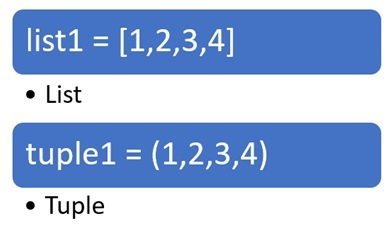
\includegraphics[width=0.5\textwidth]{figures/Difference-Between-List-and-Tuple-fig-1-2.jpg}
\caption{At first glance list and tuples look very similar, but they are not\ldots{}}
\end{figure}

Like lists, tuples are containers of any type of object. Unlike lists though they are \emph{immutable} which means that once they have been created the content cannot be changed (i.e.~no append, insert or delete of the elements). Furthermore since they are immutable they can be used as dictionary keys (lists cannot).
To create a tuple the comma-separated list of items has to be enclosed in brackets, or the $\tt{tuple()}$ operator can be used.
Accessing tuple items is done in exactly the same way as lists.

\begin{tcolorbox}[breakable, size=fbox, boxrule=1pt, pad at break*=1mm, colback=cellbackground, colframe=cellborder]
\begin{Verbatim}[commandchars=\\\{\}]
\PY{n}{atuple} \PY{o}{=} \PY{p}{(}\PY{l+m+mi}{1}\PY{p}{,} \PY{l+m+mi}{2}\PY{p}{,} \PY{l+m+mi}{3}\PY{p}{)}
\PY{n+nb}{print} \PY{p}{(}\PY{l+s+s2}{\PYZdq{}}\PY{l+s+s2}{Length: }\PY{l+s+si}{\PYZob{}\PYZcb{}}\PY{l+s+s2}{\PYZdq{}}\PY{o}{.}\PY{n}{format}\PY{p}{(}\PY{n+nb}{len}\PY{p}{(}\PY{n}{atuple}\PY{p}{)}\PY{p}{)}\PY{p}{)}
\PY{n+nb}{print} \PY{p}{(}\PY{l+s+s2}{\PYZdq{}}\PY{l+s+s2}{First element: }\PY{l+s+si}{\PYZob{}\PYZcb{}}\PY{l+s+s2}{\PYZdq{}}\PY{o}{.}\PY{n}{format}\PY{p}{(}\PY{n}{atuple}\PY{p}{[}\PY{l+m+mi}{0}\PY{p}{]}\PY{p}{)}\PY{p}{)}
\PY{n+nb}{print} \PY{p}{(}\PY{l+s+s2}{\PYZdq{}}\PY{l+s+s2}{Last element: }\PY{l+s+si}{\PYZob{}\PYZcb{}}\PY{l+s+s2}{\PYZdq{}}\PY{o}{.}\PY{n}{format}\PY{p}{(}\PY{n}{atuple}\PY{p}{[}\PY{o}{\PYZhy{}}\PY{l+m+mi}{1}\PY{p}{]}\PY{p}{)}\PY{p}{)}

Length: 3
First element: 1
Last element: 3
\end{Verbatim}
\end{tcolorbox}

In the next snippet of code it is shown the so called unpacking which is another way to assign tuple values to variables.

\begin{tcolorbox}[breakable, size=fbox, boxrule=1pt, pad at break*=1mm, colback=cellbackground, colframe=cellborder]
\begin{Verbatim}[commandchars=\\\{\}]
\PY{n}{x}\PY{p}{,} \PY{n}{y}\PY{p}{,} \PY{n}{z} \PY{o}{=} \PY{p}{(}\PY{l+m+mi}{10}\PY{p}{,} \PY{l+m+mi}{5}\PY{p}{,} \PY{l+m+mi}{12}\PY{p}{)}
\PY{n+nb}{print} \PY{p}{(}\PY{l+s+s2}{\PYZdq{}}\PY{l+s+s2}{coord: x=}\PY{l+s+si}{\PYZob{}\PYZcb{}}\PY{l+s+s2}{ y=}\PY{l+s+si}{\PYZob{}\PYZcb{}}\PY{l+s+s2}{ z=}\PY{l+s+si}{\PYZob{}\PYZcb{}}\PY{l+s+s2}{\PYZdq{}}\PY{o}{.}\PY{n}{format}\PY{p}{(}\PY{n}{x}\PY{p}{,} \PY{n}{y}\PY{p}{,} \PY{n}{z}\PY{p}{)}\PY{p}{)}

coord: x=10 y=5 z=12
\end{Verbatim}
\end{tcolorbox}

If an ntuple has just one element don't forget the comma at the end otherwise it will be treated as a single number.

\begin{tcolorbox}[breakable, size=fbox, boxrule=1pt, pad at break*=1mm, colback=cellbackground, colframe=cellborder]
\begin{Verbatim}[commandchars=\\\{\}]
\PY{n}{tuple2} \PY{o}{=} \PY{p}{(}\PY{l+m+mi}{1}\PY{p}{,}\PY{p}{)}
\PY{n+nb}{print}\PY{p}{(}\PY{n+nb}{type}\PY{p}{(}\PY{n}{tuple2}\PY{p}{)}\PY{p}{)}
\PY{n}{tuple2} \PY{o}{=} \PY{p}{(}\PY{l+m+mi}{1}\PY{p}{)}
\PY{n+nb}{print}\PY{p}{(}\PY{n+nb}{type}\PY{p}{(}\PY{n}{tuple2}\PY{p}{)}\PY{p}{)}

<class 'tuple'>
<class 'int'>
\end{Verbatim}
\end{tcolorbox}

Since a tuple is immutable to add new elements it is necessary to create a new object:

\begin{tcolorbox}[breakable, size=fbox, boxrule=1pt, pad at break*=1mm, colback=cellbackground, colframe=cellborder]\begin{Verbatim}[commandchars=\\\{\}]
\PY{n}{tuple1} \PY{o}{=} \PY{p}{(}\PY{l+m+mi}{1}\PY{p}{,} \PY{l+m+mi}{2}\PY{p}{,} \PY{l+m+mi}{3}\PY{p}{)}
\PY{n}{tuple2} \PY{o}{=} \PY{n}{tuple1} \PY{o}{+} \PY{p}{(}\PY{l+m+mi}{4}\PY{p}{,} \PY{l+m+mi}{5}\PY{p}{)}
\PY{n+nb}{print}\PY{p}{(}\PY{n}{tuple2}\PY{p}{)}

(1,2,3,4,5)
\end{Verbatim}
\end{tcolorbox}

Finally, as already said tuples can be used as dictionary keys:

\begin{tcolorbox}[breakable, size=fbox, boxrule=1pt, pad at break*=1mm, colback=cellbackground, colframe=cellborder]\begin{Verbatim}[commandchars=\\\{\}]
\PY{n}{d} \PY{o}{=} \PY{p}{\PYZob{}}
   \PY{p}{(}\PY{l+s+s1}{\PYZsq{}}\PY{l+s+s1}{Finance}\PY{l+s+s1}{\PYZsq{}}\PY{p}{,} \PY{l+m+mi}{1}\PY{p}{)}\PY{p}{:} \PY{l+s+s1}{\PYZsq{}}\PY{l+s+s1}{Room 8}\PY{l+s+s1}{\PYZsq{}}\PY{p}{,}
    \PY{p}{(}\PY{l+s+s1}{\PYZsq{}}\PY{l+s+s1}{Finance}\PY{l+s+s1}{\PYZsq{}}\PY{p}{,} \PY{l+m+mi}{2}\PY{p}{)}\PY{p}{:} \PY{l+s+s1}{\PYZsq{}}\PY{l+s+s1}{Room 3}\PY{l+s+s1}{\PYZsq{}}\PY{p}{,}
    \PY{p}{(}\PY{l+s+s1}{\PYZsq{}}\PY{l+s+s1}{Math}\PY{l+s+s1}{\PYZsq{}}\PY{p}{,} \PY{l+m+mi}{1}\PY{p}{)}\PY{p}{:} \PY{l+s+s1}{\PYZsq{}}\PY{l+s+s1}{Room 6}\PY{l+s+s1}{\PYZsq{}}\PY{p}{,}
    \PY{p}{(}\PY{l+s+s1}{\PYZsq{}}\PY{l+s+s1}{Programming}\PY{l+s+s1}{\PYZsq{}}\PY{p}{,} \PY{l+m+mi}{1}\PY{p}{)}\PY{p}{:} \PY{l+s+s1}{\PYZsq{}}\PY{l+s+s1}{IT room}\PY{l+s+s1}{\PYZsq{}}
    \PY{p}{\PYZcb{}}
\end{Verbatim}
\end{tcolorbox}

Below the full list of tuple functions:
\begin{tcolorbox}[breakable, size=fbox, boxrule=1pt, pad at break*=1mm,colback=cellbackground, colframe=cellborder]
\begin{Verbatim}[commandchars=\\\{\}]
\PY{n+nb}{dir}\PY{p}{(}\PY{n+nb}{dict}\PY{p}{)}

[...
 'count',
 'index']
\end{Verbatim}
\end{tcolorbox}

%\begin{thebibliography}{9}
%  %\bibitem{survey2019} StackOverflow \emph{The TEXbook}, Addison-Wesley, Reading,Massachusetts, second edition, 1984,
%\bibitem{survey2019} \emph{https://insights.stackoverflow.com/survey/2019}, Stack Overflow, 2019 [Online]
%\bibitem{python_versions} \emph{https://www.python.org/downloads/}, \texttt{python.org} [Online]
%\bibitem{learn_python} \emph{https://www.learnpython.org/it/}, \texttt{learnpython.org} [Online]
%\bibitem{freecamp} \emph{https://www.youtube.com/watch?v=8DvywoWv6fI}, \textt{freeCodeCamp.org} [Online]
%\bibitem{modules} \emph{https://docs.python.org/3/py-modindex.html}, Complete list of \texttt{python} modules [Online]
%\end{thebibliography}
%

\clearpage
\chapter{Data Manipulation and Its Representation}

In this chapter a closer look two a couple more of modules is given. These modules will result to be very useful in managing financial data and to report result of our analysis.

\section{Getting Data}\label{getting-data}

The first step of any analysis is usually the one that involves selection and manipulation of data we want to process. Data sources can be various (eg. website, figures, twitter messages, CSV or Excel files\ldots{}) and partially reflect its nature which can range from \emph{unstructured} data (whitout any inherent structure, e.g.~social media data) to completely \emph{structured} data (where the data model is defined and usually there is no error associated, e.g.~stock trading data).

Our primary goal, before start processing data, is to collect and store the information in a suitable data structure. \texttt{Python} provides a very useful module, called \texttt{pandas}, which allows to collect and save data in \emph{dataframe} objects that can be later on manipulated for analysis purposes.

Looking at \texttt{pandas} manual dataframe are defined as multi-dimensional, size-mutable, potentially heterogenous, tabular data structure with labeled axes (rows and columns), in much simpler words it is a table whose structure can be modified.
It presents data in a way that is suitable for data analysis, contains multiple methods for convenient data filtering and in addition has a lot of utilities to load and save data pretty easly.

Dataframes can be created by:
\begin{itemize}
\item importing data from file;
\item creating by hand data and then filling the dataframe.
\end{itemize}


\begin{tcolorbox}[breakable, size=fbox, boxrule=1pt, pad at break*=1mm,colback=cellbackground, colframe=cellborder]
\begin{Verbatim}[commandchars=\\\{\}]
\PY{k+kn}{import} \PY{n+nn}{pandas} \PY{k}{as} \PY{n+nn}{pd}

\PY{c+c1}{\PYZsh{} reading from file}
\PY{n}{df1} \PY{o}{=} \PY{n}{pd}\PY{o}{.}\PY{n}{read\PYZus{}excel}\PY{p}{(}\PY{l+s+s1}{\PYZsq{}}\PY{l+s+s1}{sample.xlsx}\PY{l+s+s1}{\PYZsq{}}\PY{p}{)} \PY{c+c1}{\PYZsh{} Excel file}
\PY{n}{df2} \PY{o}{=} \PY{n}{pd}\PY{o}{.}\PY{n}{read\PYZus{}csv}\PY{p}{(}\PY{l+s+s1}{\PYZsq{}}\PY{l+s+s1}{sample.csv}\PY{l+s+s1}{\PYZsq{}}\PY{p}{)} \PY{c+c1}{\PYZsh{} Comma Separeted file}

\PY{n}{df1}\PY{o}{.}\PY{n}{head}\PY{p}{(}\PY{l+m+mi}{11}\PY{p}{)} \PY{c+c1}{\PYZsh{} show just few rows at the beginning}

         Date       Price      Volume
0  2000-07-30  100.000000  191.811275
1  2000-07-31  129.216267  190.897541
2  2000-08-01  147.605516  197.476379
3  2000-08-02  107.282251  199.660061
4  2000-08-03  106.036826  200.840459
5  2000-08-04  118.872757  197.130212
6  2000-08-05  101.904544  204.552521
7  2000-08-06  106.392901  198.160030
8  2000-08-06  106.392901  191.125969
9  2000-08-06  106.392901  196.719061
10 2000-08-06  106.392901  196.759837
\end{Verbatim}
\end{tcolorbox}

\begin{tcolorbox}[breakable, size=fbox, boxrule=1pt, pad at break*=1mm,colback=cellbackground, colframe=cellborder]
\begin{Verbatim}[commandchars=\\\{\}]
\PY{c+c1}{\PYZsh{} creating some data in a dictionary}
\PY{n}{d} \PY{o}{=} \PY{p}{\PYZob{}}\PY{l+s+s2}{\PYZdq{}}\PY{l+s+s2}{Nome}\PY{l+s+s2}{\PYZdq{}}\PY{p}{:}\PY{p}{[}\PY{l+s+s2}{\PYZdq{}}\PY{l+s+s2}{Elisa}\PY{l+s+s2}{\PYZdq{}}\PY{p}{,} \PY{l+s+s2}{\PYZdq{}}\PY{l+s+s2}{Roberto}\PY{l+s+s2}{\PYZdq{}}\PY{p}{,} \PY{l+s+s2}{\PYZdq{}}\PY{l+s+s2}{Ciccio}\PY{l+s+s2}{\PYZdq{}}\PY{p}{,} \PY{l+s+s2}{\PYZdq{}}\PY{l+s+s2}{Topolino}\PY{l+s+s2}{\PYZdq{}}\PY{p}{,} \PY{l+s+s2}{\PYZdq{}}\PY{l+s+s2}{Gigi}\PY{l+s+s2}{\PYZdq{}}\PY{p}{]}\PY{p}{,}
     \PY{l+s+s2}{\PYZdq{}}\PY{l+s+s2}{Età}\PY{l+s+s2}{\PYZdq{}}\PY{p}{:}\PY{p}{[}\PY{l+m+mi}{1}\PY{p}{,} \PY{l+m+mi}{27}\PY{p}{,} \PY{l+m+mi}{25}\PY{p}{,} \PY{l+m+mi}{24}\PY{p}{,} \PY{l+m+mi}{31}\PY{p}{]}\PY{p}{,}
     \PY{l+s+s2}{\PYZdq{}}\PY{l+s+s2}{Punteggio}\PY{l+s+s2}{\PYZdq{}}\PY{p}{:}\PY{p}{[}\PY{l+m+mi}{100}\PY{p}{,} \PY{l+m+mi}{120}\PY{p}{,} \PY{l+m+mi}{95}\PY{p}{,} \PY{l+m+mi}{1300}\PY{p}{,} \PY{l+m+mi}{101}\PY{p}{]}\PY{p}{\PYZcb{}}

\PY{c+c1}{\PYZsh{} filling the dataframe}
\PY{n}{df} \PY{o}{=} \PY{n}{pd}\PY{o}{.}\PY{n}{DataFrame}\PY{p}{(}\PY{n}{d}\PY{p}{)}
\PY{n}{df}\PY{o}{.}\PY{n}{head}\PY{p}{(}\PY{p}{)}

       Nome  Età  Punteggio
0     Elisa    1        100
1   Roberto   27        120
2    Ciccio   25         95
3  Topolino   24       1300
4      Gigi   31        101
\end{Verbatim}
\end{tcolorbox}

Of course with \texttt{pandas} it is possible to perform a large number of operations on a dataframe. For example it is possible to add a column as a result of an operation on other columns. Looking back at the \texttt{df1} dataframe it is possible to add a column with the daily variation of the price.

\begin{tcolorbox}[breakable, size=fbox, boxrule=1pt, pad at break*=1mm,colback=cellbackground, colframe=cellborder]
\begin{Verbatim}[commandchars=\\\{\}]
\PY{k+kn}{import} \PY{n+nn}{numpy} \PY{k}{as} \PY{n+nn}{np}

\PY{c+c1}{\PYZsh{} first let\PYZsq{}s add an empty column}
\PY{n}{df1}\PY{p}{[}\PY{l+s+s1}{\PYZsq{}}\PY{l+s+s1}{Variation}\PY{l+s+s1}{\PYZsq{}}\PY{p}{]} \PY{o}{=} \PY{n}{np}\PY{o}{.}\PY{n}{nan} \PY{c+c1}{\PYZsh{} nan stands for not a number}

\PY{c+c1}{\PYZsh{} loop on the Price column, compute the variation and fill the column}
\PY{c+c1}{\PYZsh{} len returns the number of rows of a dataframe}
\PY{k}{for} \PY{n}{i} \PY{o+ow}{in} \PY{n+nb}{range}\PY{p}{(}\PY{l+m+mi}{1}\PY{p}{,} \PY{n+nb}{len}\PY{p}{(}\PY{n}{df1}\PY{p}{)}\PY{p}{)}\PY{p}{:}
    \PY{c+c1}{\PYZsh{} select the ith row and fill \PYZdq{}Variation\PYZdq{}}
    \PY{c+c1}{\PYZsh{} loc takes as inputs row and colum\PYZhy{}name}
    \PY{n}{df1}\PY{o}{.}\PY{n}{loc}\PY{p}{[}\PY{n}{i}\PY{p}{,} \PY{l+s+s2}{\PYZdq{}}\PY{l+s+s2}{Variation}\PY{l+s+s2}{\PYZdq{}}\PY{p}{]} \PY{o}{=} \PY{p}{(}\PY{n}{df1}\PY{o}{.}\PY{n}{loc}\PY{p}{[}\PY{n}{i}\PY{p}{,} \PY{l+s+s2}{\PYZdq{}}\PY{l+s+s2}{Price}\PY{l+s+s2}{\PYZdq{}}\PY{p}{]} \PY{o}{\PYZhy{}} \PY{n}{df1}\PY{o}{.}\PY{n}{loc}\PY{p}{[}\PY{n}{i}\PY{o}{\PYZhy{}}\PY{l+m+mi}{1}\PY{p}{,} \PY{l+s+s2}{\PYZdq{}}\PY{l+s+s2}{Price}\PY{l+s+s2}{\PYZdq{}}\PY{p}{]}\PY{p}{)} \PY{o}{/}
                      \PY{n}{df1}\PY{o}{.}\PY{n}{loc}\PY{p}{[}\PY{n}{i}\PY{o}{\PYZhy{}}\PY{l+m+mi}{1}\PY{p}{,} \PY{l+s+s2}{\PYZdq{}}\PY{l+s+s2}{Price}\PY{l+s+s2}{\PYZdq{}}\PY{p}{]}

\PY{n}{df1}\PY{o}{.}\PY{n}{head}\PY{p}{(}\PY{p}{)}

        Date       Price      Volume  Variation
0 2000-07-30  100.000000  191.811275        NaN
1 2000-07-31  129.216267  190.897541   0.292163
2 2000-08-01  147.605516  197.476379   0.142314
3 2000-08-02  107.282251  199.660061  -0.273183
4 2000-08-03  106.036826  200.840459  -0.011609
\end{Verbatim}
\end{tcolorbox}

Of course the first ``variation'' value is NaN since there is no previous price to compare with.

\subsection{Manage Data}\label{manage-data}

Once we have created our dataframe we may want to preliminarly process data to perform very common operations like:

\begin{itemize}
\item remove unwanted observations or outliers;
\item handle missing data;
\item filter, sort and clean data.
\end{itemize}

\subsection{Unwanted observations and outliers}

\subsubsection{Duplicates}

It may happen that our data has duplicates (e.g.~those can arise when combining two datasets), or the dataset contains irrelvant fields for the specific study we are carrying on. To find and remove duplicates \texttt{pandas} has convenient methods:

\begin{tcolorbox}[breakable, size=fbox, boxrule=1pt, pad at break*=1mm,colback=cellbackground, colframe=cellborder]
\begin{Verbatim}[commandchars=\\\{\}]
\PY{c+c1}{\PYZsh{} find duplicates based on all columns}
\PY{c+c1}{\PYZsh{} and show just the first 15 results  }
\PY{c+c1}{\PYZsh{}print (df1.duplicated()[:15]) }

\PY{c+c1}{\PYZsh{} find duplicates based on\PYZsq{}Price\PYZsq{}}
\PY{c+c1}{\PYZsh{} and show just the first 15 results}
\PY{n+nb}{print} \PY{p}{(}\PY{n}{df1}\PY{o}{.}\PY{n}{duplicated}\PY{p}{(}\PY{n}{subset}\PY{o}{=}\PY{p}{[}\PY{l+s+s1}{\PYZsq{}}\PY{l+s+s1}{Price}\PY{l+s+s1}{\PYZsq{}}\PY{p}{]}\PY{p}{)}\PY{p}{[}\PY{p}{:}\PY{l+m+mi}{15}\PY{p}{]} \PY{p}{)}

0     False
1     False
2     False
3     False
4     False
5     False
6     False
7     False
8      True
9      True
10     True
11    False
12    False
13    False
14    False
dtype: bool
\end{Verbatim}
\end{tcolorbox}












\begin{tcolorbox}[breakable, size=fbox, boxrule=1pt, pad at break*=1mm,colback=cellbackground, colframe=cellborder]
\begin{Verbatim}[commandchars=\\\{\}]
\PY{n+nb}{print} \PY{p}{(}\PY{l+s+s2}{\PYZdq{}}\PY{l+s+s2}{Initial number of rows: }\PY{l+s+si}{\PYZob{}\PYZcb{}}\PY{l+s+s2}{\PYZdq{}}\PY{o}{.}\PY{n}{format}\PY{p}{(}\PY{n+nb}{len}\PY{p}{(}\PY{n}{df1}\PY{p}{)}\PY{p}{)}\PY{p}{)} 

\PY{c+c1}{\PYZsh{} remove duplicates}
\PY{c+c1}{\PYZsh{} where the second argument can be `first`, `last` }
\PY{c+c1}{\PYZsh{} or `False` (consider all of the same values as duplicates).}
\PY{n}{df1} \PY{o}{=} \PY{n}{df1}\PY{o}{.}\PY{n}{drop\PYZus{}duplicates}\PY{p}{(}\PY{n}{subset}\PY{o}{=}\PY{l+s+s1}{\PYZsq{}}\PY{l+s+s1}{Price}\PY{l+s+s1}{\PYZsq{}}\PY{p}{,} \PY{n}{keep}\PY{o}{=}\PY{l+s+s1}{\PYZsq{}}\PY{l+s+s1}{first}\PY{l+s+s1}{\PYZsq{}}\PY{p}{)}

\PY{n+nb}{print} \PY{p}{(}\PY{l+s+s2}{\PYZdq{}}\PY{l+s+s2}{Number of columns after drop: }\PY{l+s+si}{\PYZob{}\PYZcb{}}\PY{l+s+s2}{\PYZdq{}}\PY{o}{.}\PY{n}{format}\PY{p}{(}\PY{n+nb}{len}\PY{p}{(}\PY{n}{df1}\PY{p}{)}\PY{p}{)}\PY{p}{)}

Initial number of rows: 734
Number of columns after drop: 729
\end{Verbatim}
\end{tcolorbox}

If we would like to drop irrilevant columns for our analysis it is enough to:

\begin{tcolorbox}[breakable, size=fbox, boxrule=1pt, pad at break*=1mm,colback=cellbackground, colframe=cellborder]
\begin{Verbatim}[commandchars=\\\{\}]
\PY{n}{df2} \PY{o}{=} \PY{n}{df2}\PY{o}{.}\PY{n}{drop}\PY{p}{(}\PY{n}{columns}\PY{o}{=}\PY{p}{[}\PY{l+s+s1}{\PYZsq{}}\PY{l+s+s1}{Volume}\PY{l+s+s1}{\PYZsq{}}\PY{p}{]}\PY{p}{)}
\PY{n}{df2}\PY{o}{.}\PY{n}{head}\PY{p}{(}\PY{p}{)}

         Date       Price
0  2000-07-30  100.000000
1  2000-07-31  129.216267
2  2000-08-01  147.605516
3  2000-08-02  107.282251
4  2000-08-03  106.036826
\end{Verbatim}
\end{tcolorbox}
        
If instead we just want to remove few rows we can select them by index:

\begin{tcolorbox}[breakable, size=fbox, boxrule=1pt, pad at break*=1mm,colback=cellbackground, colframe=cellborder]
\begin{Verbatim}[commandchars=\\\{\}]
\PY{c+c1}{\PYZsh{} we remove row 0th and 2nd}
\PY{c+c1}{\PYZsh{} axis=0 means use the index column}
\PY{n}{df2} \PY{o}{=} \PY{n}{df2}\PY{o}{.}\PY{n}{drop}\PY{p}{(}\PY{p}{[}\PY{l+m+mi}{0}\PY{p}{,} \PY{l+m+mi}{2}\PY{p}{]}\PY{p}{,} \PY{n}{axis}\PY{o}{=}\PY{l+m+mi}{0}\PY{p}{)}
\PY{n}{df2}\PY{o}{.}\PY{n}{head}\PY{p}{(}\PY{p}{)}

         Date       Price
1  2000-07-31  129.216267
3  2000-08-02  107.282251
4  2000-08-03  106.036826
5  2000-08-04  118.872757
6  2000-08-05  101.904544
\end{Verbatim}
\end{tcolorbox}
        
Changing the column that act as index we can select the rows also by other attributes:

\begin{tcolorbox}[breakable, size=fbox, boxrule=1pt, pad at break*=1mm,colback=cellbackground, colframe=cellborder]
\begin{Verbatim}[commandchars=\\\{\}]
\PY{c+c1}{\PYZsh{} tell pandas to use Date as index column}
\PY{n}{df2} \PY{o}{=} \PY{n}{df2}\PY{o}{.}\PY{n}{set\PYZus{}index}\PY{p}{(}\PY{l+s+s1}{\PYZsq{}}\PY{l+s+s1}{Date}\PY{l+s+s1}{\PYZsq{}}\PY{p}{)}

\PY{c+c1}{\PYZsh{} select row to remove by date at this point}
\PY{n}{df2} \PY{o}{=} \PY{n}{df2}\PY{o}{.}\PY{n}{drop}\PY{p}{(}\PY{p}{[}\PY{l+s+s2}{\PYZdq{}}\PY{l+s+s2}{2000\PYZhy{}07\PYZhy{}31}\PY{l+s+s2}{\PYZdq{}}\PY{p}{]}\PY{p}{,} \PY{n}{axis}\PY{o}{=}\PY{l+m+mi}{0}\PY{p}{)}

\PY{n}{df2}\PY{o}{.}\PY{n}{head}\PY{p}{(}\PY{p}{)}

Date        Price
2000-08-02  107.282251
2000-08-03  106.036826
2000-08-04  118.872757
2000-08-05  101.904544
2000-08-06  106.392901
\end{Verbatim}
\end{tcolorbox}
        
\subsubsection{Outliers}\label{outliers}

An outlier is an observation that lies outside the overall pattern of a distribution. Common causes can be human, measurement or experimental errors. Outliers must be handled carefully and we should remove them cautiously, \emph{outliers are innocent until proven guilty}. We may have removed the most interesting part of our dataset !

The core statistics about a particular column can be studied by the \texttt{describe()} method which returns the following information:
\begin{itemize}
\item for numeric columns: the value count, mean, standard deviation, minimum, maximum and 25th, 50th and 75h quantiles for the data in a column;
\item for string columns: the number of unique entries, the most frequent occurring value (\emph{top}), and the number of times the top value occurs (\emph{freq}).
\end{itemize}

\begin{tcolorbox}[breakable, size=fbox, boxrule=1pt, pad at break*=1mm,colback=cellbackground, colframe=cellborder]
\begin{Verbatim}[commandchars=\\\{\}]
\PY{n}{df1}\PY{o}{.}\PY{n}{describe}\PY{p}{(}\PY{p}{)}

              Price      Volume   Variation
count    728.000000  729.000000  724.000000
mean     120.898678  200.355900    0.146330
std      490.493411    4.970745    3.637952
min        0.878873  186.430551   -0.995284
25\%       14.809934  196.998603   -0.119423
50\%       61.325699  200.221125   -0.005549
75\%      164.021813  203.580691    0.121290
max    13000.000000  215.140868   97.756432
\end{Verbatim}
\end{tcolorbox}
        
Looking at mean and std and comparing it with min and max values we could find a range outside of which we may have outliers. For example 13000.0 is several standard deviation away the mean which may indicate that it is not a good value.

Another way to spot outliers is to plot column distributions and again \texttt{pandas} comes to help us:

\begin{tcolorbox}[breakable, size=fbox, boxrule=1pt, pad at break*=1mm,colback=cellbackground, colframe=cellborder]
\begin{Verbatim}[commandchars=\\\{\}]
\PY{n}{df1}\PY{o}{.}\PY{n}{hist}\PY{p}{(}\PY{l+s+s2}{\PYZdq{}}\PY{l+s+s2}{Variation}\PY{l+s+s2}{\PYZdq{}}\PY{p}{,} \PY{n}{bins}\PY{o}{=}\PY{n}{np}\PY{o}{.}\PY{n}{arange}\PY{p}{(}\PY{l+m+mi}{0}\PY{p}{,} \PY{l+m+mi}{100}\PY{p}{,} \PY{l+m+mi}{1}\PY{p}{)}\PY{p}{)}

---------------------------------------------------------------------------

NameError                                 Traceback (most recent call last)

        <ipython-input-1-97dbdc6fcfec> in <module>
    ----> 1 df1.hist("Variation", bins=np.arange(0, 100, 1))
    

        NameError: name 'df1' is not defined
\end{Verbatim}
\end{tcolorbox}

From the histograms it is clear how the value of 97.76, is far from general population. This doesn't mean they are necessarily wrong but it should make ring a bell in our head\ldots{}

To remove outliers from data we can either remove the entire rows or replace the suspicious values by a default value (e.g.~0, 1, a threshold value\ldots{}).

\textbf{Note}:~missing data may be informative itself~!~When filling the gap with \emph{artificial data} (e.g.~mean, median, std\ldots{}) having similar properties than real observation, the added value won't be scientifically valid, no matter how sophisticated your filling method is.

\begin{Shaded}
\begin{Highlighting}[]
\ImportTok{import}\NormalTok{ numpy }\ImportTok{as}\NormalTok{ np}

\NormalTok{df2.replace(}\DecValTok{1300}\NormalTok{, }\DecValTok{500}\NormalTok{)      }\CommentTok{# replace 1300 with 500}
\NormalTok{df2 }\OperatorTok{=}\NormalTok{ df2.replace(}\DecValTok{1300}\NormalTok{, np.nan)   }\CommentTok{# replace 1300 with NaN}

\NormalTok{df2 }\OperatorTok{=}\NormalTok{ df2.mask(df1 }\OperatorTok{>=} \DecValTok{600}\NormalTok{, }\DecValTok{500}\NormalTok{)   }\CommentTok{# replace every element >=600 with 5}
\end{Highlighting}
\end{Shaded}

\subsection{Handle Missing Data}\label{handle-missing-data}

Usually when importing data with \texttt{pandas} we may have some NaN values (short for \emph{not a number} which represent the \texttt{null} value). NaN is the value that is given to missing fields in a row. Like for the outliers we can use the \texttt{replace} or \texttt{mask} methods to remove the NaNs. In case the whole row as NaN it may be wise to drop it entirely.

Additionally we can use \texttt{dropna()} which remove all the NaN at once.

\begin{tcolorbox}[breakable, size=fbox, boxrule=1pt, pad at break*=1mm,colback=cellbackground, colframe=cellborder]
\begin{Verbatim}[commandchars=\\\{\}]
\PY{n}{df1} \PY{o}{=} \PY{n}{df1}\PY{o}{.}\PY{n}{dropna}\PY{p}{(}\PY{p}{)}

\PY{n+nb}{print} \PY{p}{(}\PY{l+s+s2}{\PYZdq{}}\PY{l+s+s2}{Number of rows after dropping NaN: }\PY{l+s+si}{\PYZob{}\PYZcb{}}\PY{l+s+s2}{\PYZdq{}}\PY{o}{.}\PY{n}{format}\PY{p}{(}\PY{n+nb}{len}\PY{p}{(}\PY{n}{df1}\PY{p}{)}\PY{p}{)}\PY{p}{)}

Number of rows after dropping NaN: 724
\end{Verbatim}
\end{tcolorbox}

\subsection{Filter, Sort and Clean Data}\label{filter-sort-and-clean-data}

\subsubsection{Filtering}\label{filtering}

When we work with huge datasets we may reach computational limits (e.g.~insufficient memory, CPU performance, too slow processing time\ldots{}) and in those cases it can be helpful to filter data by attributes for example by splitting by time or some other property.

Assuming to have the following table and putting back the volume column

\begin{tcolorbox}[breakable, size=fbox, boxrule=1pt, pad at break*=1mm,colback=cellbackground, colframe=cellborder]
\begin{Verbatim}[commandchars=\\\{\}]
\PY{c+c1}{\PYZsh{} df.iloc[row, col]}
\PY{c+c1}{\PYZsh{} NOTE: iloc takes row and column index (two numbers)}
\PY{c+c1}{\PYZsh{} loc instead takes row index and column name}
\PY{n+nb}{print} \PY{p}{(}\PY{n}{df1}\PY{o}{.}\PY{n}{iloc}\PY{p}{[}\PY{l+m+mi}{1}\PY{p}{,} \PY{l+m+mi}{2}\PY{p}{]}\PY{p}{)} \PY{c+c1}{\PYZsh{} returns 62 the volume associated with the row 1}

\PY{n+nb}{print}\PY{p}{(}\PY{p}{)}
\PY{c+c1}{\PYZsh{}df.iloc[row1:row2, col1:col2]}
\PY{c+c1}{\PYZsh{} this is called slicing, remember ?}
\PY{n+nb}{print} \PY{p}{(}\PY{n}{df1}\PY{o}{.}\PY{n}{iloc}\PY{p}{[}\PY{l+m+mi}{0}\PY{p}{:}\PY{l+m+mi}{2}\PY{p}{,} \PY{l+m+mi}{2}\PY{p}{:}\PY{l+m+mi}{3}\PY{p}{]}\PY{p}{)} \PY{c+c1}{\PYZsh{} returns rows 0 and 1 of column 2}

197.476378531652

       Volume
1  190.897541
2  197.476379
\end{Verbatim}
\end{tcolorbox}

\begin{tcolorbox}[breakable, size=fbox, boxrule=1pt, pad at break*=1mm,colback=cellbackground, colframe=cellborder]
\begin{Verbatim}[commandchars=\\\{\}]
\PY{n}{subset} \PY{o}{=} \PY{n}{df1}\PY{o}{.}\PY{n}{iloc}\PY{p}{[}\PY{p}{:}\PY{p}{,} \PY{l+m+mi}{1}\PY{p}{]}   \PY{c+c1}{\PYZsh{} select column 1}

\PY{n}{subset} \PY{o}{=} \PY{n}{df1}\PY{o}{.}\PY{n}{iloc}\PY{p}{[}\PY{l+m+mi}{2}\PY{p}{,} \PY{p}{:}\PY{p}{]}   \PY{c+c1}{\PYZsh{} select row 2}

\PY{n}{subset} \PY{o}{=} \PY{n}{df1}\PY{o}{.}\PY{n}{iloc}\PY{p}{[}\PY{l+m+mi}{0}\PY{p}{:}\PY{l+m+mi}{2}\PY{p}{,} \PY{p}{:}\PY{p}{]} \PY{c+c1}{\PYZsh{} select 2 rows}

\PY{n}{subset} \PY{o}{=} \PY{n}{df1}\PY{o}{.}\PY{n}{iloc}\PY{p}{[}\PY{p}{:}\PY{l+m+mi}{2}\PY{p}{,} \PY{p}{:}\PY{p}{]}  \PY{c+c1}{\PYZsh{} this is equivalent to before}
\end{Verbatim}
\end{tcolorbox}

A more advanced way of filtering is the following (it apply a selection on the values). The notation is a bit awkward but very useful:

\begin{tcolorbox}[breakable, size=fbox, boxrule=1pt, pad at break*=1mm,colback=cellbackground, colframe=cellborder]
\begin{Verbatim}[commandchars=\\\{\}]
\PY{k+kn}{import} \PY{n+nn}{datetime}

\PY{c+c1}{\PYZsh{} colon means all the rows}
\PY{n}{subset} \PY{o}{=} \PY{n}{df1}\PY{p}{[}\PY{n}{df1}\PY{o}{.}\PY{n}{iloc}\PY{p}{[}\PY{p}{:}\PY{p}{,} \PY{l+m+mi}{0}\PY{p}{]} \PY{o}{\PYZlt{}} \PY{n}{datetime}\PY{o}{.}\PY{n}{datetime}\PY{p}{(}\PY{l+m+mi}{2000}\PY{p}{,} \PY{l+m+mi}{8}\PY{p}{,} \PY{l+m+mi}{15}\PY{p}{)}\PY{p}{]}
\PY{n+nb}{print} \PY{p}{(}\PY{n}{subset}\PY{p}{)}

         Date       Price      Volume  Variation
1  2000-07-31  129.216267  190.897541   0.292163
2  2000-08-01  147.605516  197.476379   0.142314
3  2000-08-02  107.282251  199.660061  -0.273183
4  2000-08-03  106.036826  200.840459  -0.011609
5  2000-08-04  118.872757  197.130212   0.121052
6  2000-08-05  101.904544  204.552521  -0.142743
7  2000-08-06  106.392901  198.160030   0.044045
11 2000-08-07  107.646053  198.861429   0.011779
12 2000-08-08  106.666468  197.213497  -0.009100
13 2000-08-09  101.981029  204.425797  -0.043926
14 2000-08-10  110.100330  196.122844   0.079616
15 2000-08-11  138.656481  200.703360   0.259365
16 2000-08-12  113.180782  205.676449  -0.183732
17 2000-08-13  137.639947  203.468517   0.216107
18 2000-08-14  142.646169  198.528626   0.036372
\end{Verbatim}
\end{tcolorbox}

\subsubsection{Sorting}\label{sorting}

To sort our data we can use \texttt{sort\_values()} method (it can be specified ascending, descending).

\begin{tcolorbox}[breakable, size=fbox, boxrule=1pt, pad at break*=1mm,colback=cellbackground, colframe=cellborder]
\begin{Verbatim}[commandchars=\\\{\}]
\PY{c+c1}{\PYZsh{} sort by price then by date in descending order}
\PY{n}{df2}\PY{o}{.}\PY{n}{sort\PYZus{}values}\PY{p}{(}\PY{n}{by}\PY{o}{=}\PY{p}{[}\PY{l+s+s1}{\PYZsq{}}\PY{l+s+s1}{Price}\PY{l+s+s1}{\PYZsq{}}\PY{p}{,} \PY{l+s+s2}{\PYZdq{}}\PY{l+s+s2}{Date}\PY{l+s+s2}{\PYZdq{}}\PY{p}{]}\PY{p}{,} \PY{n}{ascending}\PY{o}{=}\PY{k+kc}{False}\PY{p}{)}\PY{p}{[}\PY{p}{:}\PY{l+m+mi}{10}\PY{p}{]}

      Date         Price
2000-08-20  13000.000000
2000-10-20    593.477666
2001-01-05    571.444679
2000-12-31    532.558487
2000-10-14    516.044122
2001-01-02    503.583189
2001-01-01    502.849987
2000-12-30    487.353466
2001-01-04    478.027182
2001-01-10    473.061993
\end{Verbatim}
\end{tcolorbox}
        
\paragraph{Cleaning or Regularizing}\label{cleaning-or-regularizing}

As we will see when dealing with machine learning, often we need to regularize our data to improve the stability of a training. One typical situation is when we want to \emph{normalize} data, which means rescale the values into a range of {[}0, 1{]}.

\(x = [1,43,65,23,4,57,87,45,45,23]\)

\(x_{new} = \frac{x - x_{min}}{x_{max} - x_{min}}\)

\(x_{new} = [0,0.48,0.74,0.25,0.03,0.65,1,0.51,0.51,0.25]\)

To apply such a transformation with \texttt{pandas} is very easy since applying the formula to a dataframe implies it is done to each row:

\begin{tcolorbox}[breakable, size=fbox, boxrule=1pt, pad at break*=1mm,colback=cellbackground, colframe=cellborder]
\begin{Verbatim}[commandchars=\\\{\}]
\PY{n}{df1}\PY{p}{[}\PY{l+s+s1}{\PYZsq{}}\PY{l+s+s1}{Price}\PY{l+s+s1}{\PYZsq{}}\PY{p}{]} \PY{o}{=} \PY{p}{(}\PY{n}{df1}\PY{p}{[}\PY{l+s+s1}{\PYZsq{}}\PY{l+s+s1}{Price}\PY{l+s+s1}{\PYZsq{}}\PY{p}{]} \PY{o}{\PYZhy{}} \PY{n}{df1}\PY{p}{[}\PY{l+s+s1}{\PYZsq{}}\PY{l+s+s1}{Price}\PY{l+s+s1}{\PYZsq{}}\PY{p}{]}\PY{o}{.}\PY{n}{min}\PY{p}{(}\PY{p}{)}\PY{p}{)} \PYZbs{}
    \PY{o}{/} \PY{p}{(}\PY{n}{df1}\PY{p}{[}\PY{l+s+s1}{\PYZsq{}}\PY{l+s+s1}{Price}\PY{l+s+s1}{\PYZsq{}}\PY{p}{]}\PY{o}{.}\PY{n}{max}\PY{p}{(}\PY{p}{)} \PY{o}{\PYZhy{}} \PY{n}{df1}\PY{p}{[}\PY{l+s+s1}{\PYZsq{}}\PY{l+s+s1}{Price}\PY{l+s+s1}{\PYZsq{}}\PY{p}{]}\PY{o}{.}\PY{n}{min}\PY{p}{(}\PY{p}{)}\PY{p}{)}
\PY{n}{df1}\PY{o}{.}\PY{n}{head}\PY{p}{(}\PY{p}{)}

        Date     Price      Volume  Variation
1 2000-07-31  0.009873  190.897541   0.292163
2 2000-08-01  0.011287  197.476379   0.142314
3 2000-08-02  0.008185  199.660061  -0.273183
4 2000-08-03  0.008090  200.840459  -0.011609
5 2000-08-04  0.009077  197.130212   0.121052
\end{Verbatim}
\end{tcolorbox}
        
Another quite common transfrmation is called \emph{standardization}, essentially we rescale data to have 0 mean and standard deviation of 1:

\(x_{new} = \frac{x-\mu}{\sigma}\)

Again it is straightforward to do it in \texttt{pandas}:

\begin{tcolorbox}[breakable, size=fbox, boxrule=1pt, pad at break*=1mm,colback=cellbackground, colframe=cellborder]
\begin{Verbatim}[commandchars=\\\{\}]
\PY{n}{df1}\PY{o}{.}\PY{n}{hist}\PY{p}{(}\PY{l+s+s1}{\PYZsq{}}\PY{l+s+s1}{Volume}\PY{l+s+s1}{\PYZsq{}}\PY{p}{,} \PY{n}{bins}\PY{o}{=}\PY{n}{np}\PY{o}{.}\PY{n}{arange}\PY{p}{(}\PY{l+m+mi}{180}\PY{p}{,} \PY{l+m+mi}{220}\PY{p}{,} \PY{l+m+mi}{1}\PY{p}{)}\PY{p}{)}
\PY{n+nb}{print} \PY{p}{(}\PY{n}{df1}\PY{p}{[}\PY{l+s+s1}{\PYZsq{}}\PY{l+s+s1}{Volume}\PY{l+s+s1}{\PYZsq{}}\PY{p}{]}\PY{o}{.}\PY{n}{mean}\PY{p}{(}\PY{p}{)}\PY{p}{)}
\PY{n+nb}{print} \PY{p}{(}\PY{n}{df1}\PY{p}{[}\PY{l+s+s1}{\PYZsq{}}\PY{l+s+s1}{Volume}\PY{l+s+s1}{\PYZsq{}}\PY{p}{]}\PY{o}{.}\PY{n}{std}\PY{p}{(}\PY{p}{)}\PY{p}{)}

200.36750575214748
4.968224698257929
\end{Verbatim}
\end{tcolorbox}

\begin{center}
  \adjustimage{max size={0.9\linewidth}{0.9\paperheight}}{Untitled_files/Untitled_40_1.png}
\end{center}
    { \hspace*{\fill} \\}
    
\begin{tcolorbox}[breakable, size=fbox, boxrule=1pt, pad at break*=1mm,colback=cellbackground, colframe=cellborder]
\begin{Verbatim}[commandchars=\\\{\}]
\PY{n}{df1}\PY{p}{[}\PY{l+s+s1}{\PYZsq{}}\PY{l+s+s1}{Volume}\PY{l+s+s1}{\PYZsq{}}\PY{p}{]} \PY{o}{=} \PY{p}{(}\PY{n}{df1}\PY{p}{[}\PY{l+s+s1}{\PYZsq{}}\PY{l+s+s1}{Volume}\PY{l+s+s1}{\PYZsq{}}\PY{p}{]} \PY{o}{\PYZhy{}} \PY{n}{df1}\PY{p}{[}\PY{l+s+s1}{\PYZsq{}}\PY{l+s+s1}{Volume}\PY{l+s+s1}{\PYZsq{}}\PY{p}{]}\PY{o}{.}\PY{n}{mean}\PY{p}{(}\PY{p}{)}\PY{p}{)} \PY{o}{/} \PY{n}{df1}\PY{p}{[}\PY{l+s+s1}{\PYZsq{}}\PY{l+s+s1}{Volume}\PY{l+s+s1}{\PYZsq{}}\PY{p}{]}\PY{o}{.}\PY{n}{std}\PY{p}{(}\PY{p}{)}

\PY{n}{df1}\PY{o}{.}\PY{n}{hist}\PY{p}{(}\PY{l+s+s1}{\PYZsq{}}\PY{l+s+s1}{Volume}\PY{l+s+s1}{\PYZsq{}}\PY{p}{,} \PY{n}{bins}\PY{o}{=}\PY{n}{np}\PY{o}{.}\PY{n}{arange}\PY{p}{(}\PY{o}{\PYZhy{}}\PY{l+m+mi}{5}\PY{p}{,} \PY{l+m+mi}{5}\PY{p}{,} \PY{l+m+mf}{0.1}\PY{p}{)}\PY{p}{)}
\PY{n+nb}{print} \PY{p}{(}\PY{n}{df1}\PY{p}{[}\PY{l+s+s1}{\PYZsq{}}\PY{l+s+s1}{Volume}\PY{l+s+s1}{\PYZsq{}}\PY{p}{]}\PY{o}{.}\PY{n}{mean}\PY{p}{(}\PY{p}{)}\PY{p}{)}
\PY{n+nb}{print} \PY{p}{(}\PY{n}{df1}\PY{p}{[}\PY{l+s+s1}{\PYZsq{}}\PY{l+s+s1}{Volume}\PY{l+s+s1}{\PYZsq{}}\PY{p}{]}\PY{o}{.}\PY{n}{std}\PY{p}{(}\PY{p}{)}\PY{p}{)}

-6.148550054609154e-15
1.0
\end{Verbatim}
\end{tcolorbox}

\begin{center}
  \adjustimage{max size={0.9\linewidth}{0.9\paperheight}}{Untitled_files/Untitled_41_1.png}
\end{center}
    { \hspace*{\fill} \\}
    
\section{Plotting in \texttt{python}}\label{plotting-in-python}

As we have just seen \texttt{pandas} allows to quickly draw histograms of dataframe columns, but during an analysis we may want to plot distributions from \texttt{list} or objects not stored in a dataframe. Furthermore the simple and very useful provided interface doesn't grant full access to all histogram features that we need to produce nice and informative plots.

In order to do so we can use the \texttt{matplotlib} module which is specifically dedicated to plotting (pandas interface is based on the same module indeed). Let's look briefly to its capability by examples.

\subsection{Plot a graph given \(x\) and \(y\) values (scatter-plot)}\label{plot-a-graph-given-x-and-y-values}

\begin{tcolorbox}[breakable, size=fbox, boxrule=1pt, pad at break*=1mm,colback=cellbackground, colframe=cellborder]
\begin{Verbatim}[commandchars=\\\{\}]
\PY{k+kn}{from} \PY{n+nn}{matplotlib} \PY{k}{import} \PY{n}{pyplot} \PY{k}{as} \PY{n}{plt}

\PY{n}{x} \PY{o}{=} \PY{p}{[}\PY{l+m+mi}{1}\PY{p}{,} \PY{l+m+mi}{2}\PY{p}{,} \PY{l+m+mi}{3}\PY{p}{]}
\PY{n}{y} \PY{o}{=} \PY{p}{[}\PY{l+m+mf}{0.3}\PY{p}{,} \PY{l+m+mf}{0.4}\PY{p}{,} \PY{l+m+mf}{0.6}\PY{p}{]}
 
\PY{n}{plt}\PY{o}{.}\PY{n}{plot}\PY{p}{(}\PY{n}{x}\PY{p}{,} \PY{n}{y}\PY{p}{,} \PY{n}{marker}\PY{o}{=}\PY{l+s+s1}{\PYZsq{}}\PY{l+s+s1}{o}\PY{l+s+s1}{\PYZsq{}}\PY{p}{)} \PY{c+c1}{\PYZsh{} we are using circle markers}
\PY{n}{plt}\PY{o}{.}\PY{n}{grid}\PY{p}{(}\PY{k+kc}{True}\PY{p}{)}               \PY{c+c1}{\PYZsh{} this line activate grid drawing}
\PY{n}{plt}\PY{o}{.}\PY{n}{show}\PY{p}{(}\PY{p}{)}
\end{Verbatim}
\end{tcolorbox}

\begin{center}
  \adjustimage{max size={0.9\linewidth}{0.9\paperheight}}{Untitled_files/Untitled_43_0.png}
\end{center}
    { \hspace*{\fill} \\}
    
\begin{tcolorbox}[breakable, size=fbox, boxrule=1pt, pad at break*=1mm,colback=cellbackground, colframe=cellborder]
\begin{Verbatim}[commandchars=\\\{\}]
\PY{c+c1}{\PYZsh{} if we want to plot specific points too}

\PY{n}{x} \PY{o}{=} \PY{p}{[}\PY{l+m+mi}{1}\PY{p}{,} \PY{l+m+mi}{2}\PY{p}{,} \PY{l+m+mi}{3}\PY{p}{]}
\PY{n}{y} \PY{o}{=} \PY{p}{[}\PY{l+m+mf}{0.3}\PY{p}{,} \PY{l+m+mf}{0.4}\PY{p}{,} \PY{l+m+mf}{0.6}\PY{p}{]}
 
\PY{n}{plt}\PY{o}{.}\PY{n}{plot}\PY{p}{(}\PY{n}{x}\PY{p}{,} \PY{n}{y}\PY{p}{,} \PY{n}{marker}\PY{o}{=}\PY{l+s+s1}{\PYZsq{}}\PY{l+s+s1}{x}\PY{l+s+s1}{\PYZsq{}}\PY{p}{)}
\PY{n}{plt}\PY{o}{.}\PY{n}{plot}\PY{p}{(}\PY{l+m+mf}{2.5}\PY{p}{,} \PY{l+m+mf}{0.5}\PY{p}{,} \PY{n}{marker}\PY{o}{=}\PY{l+s+s1}{\PYZsq{}}\PY{l+s+s1}{X}\PY{l+s+s1}{\PYZsq{}}\PY{p}{,} \PY{n}{ms}\PY{o}{=}\PY{l+m+mi}{12}\PY{p}{,} \PY{n}{color}\PY{o}{=}\PY{l+s+s1}{\PYZsq{}}\PY{l+s+s1}{red}\PY{l+s+s1}{\PYZsq{}}\PY{p}{)}
\PY{n}{plt}\PY{o}{.}\PY{n}{plot}\PY{p}{(}\PY{l+m+mf}{1.5}\PY{p}{,} \PY{l+m+mf}{0.35}\PY{p}{,} \PY{n}{marker}\PY{o}{=}\PY{l+s+s1}{\PYZsq{}}\PY{l+s+s1}{x}\PY{l+s+s1}{\PYZsq{}}\PY{p}{,} \PY{n}{ms}\PY{o}{=}\PY{l+m+mi}{12}\PY{p}{,} \PY{n}{color}\PY{o}{=}\PY{l+s+s1}{\PYZsq{}}\PY{l+s+s1}{red}\PY{l+s+s1}{\PYZsq{}}\PY{p}{)}
\PY{n}{plt}\PY{o}{.}\PY{n}{grid}\PY{p}{(}\PY{k+kc}{True}\PY{p}{)}              
\PY{n}{plt}\PY{o}{.}\PY{n}{show}\PY{p}{(}\PY{p}{)}
\end{Verbatim}
\end{tcolorbox}

\begin{center}
  \adjustimage{max size={0.9\linewidth}{0.9\paperheight}}{Untitled_files/Untitled_44_0.png}
\end{center}
    { \hspace*{\fill} \\}
    
\subsubsection{What if \(x\) values are dates ?}

\begin{tcolorbox}[breakable, size=fbox, boxrule=1pt, pad at break*=1mm,colback=cellbackground, colframe=cellborder]
\begin{Verbatim}[commandchars=\\\{\}]
\PY{k+kn}{import} \PY{n+nn}{datetime}
\PY{k+kn}{from} \PY{n+nn}{matplotlib} \PY{k}{import} \PY{n}{pyplot} \PY{k}{as} \PY{n}{plt}
\PY{k+kn}{import} \PY{n+nn}{matplotlib}\PY{n+nn}{.}\PY{n+nn}{dates} \PY{k}{as} \PY{n+nn}{mdates}

\PY{n}{x} \PY{o}{=} \PY{p}{[}\PY{n}{datetime}\PY{o}{.}\PY{n}{date}\PY{p}{(}\PY{l+m+mi}{2020}\PY{p}{,} \PY{l+m+mi}{7}\PY{p}{,} \PY{l+m+mi}{20}\PY{p}{)}\PY{p}{,} 
     \PY{n}{datetime}\PY{o}{.}\PY{n}{date}\PY{p}{(}\PY{l+m+mi}{2020}\PY{p}{,} \PY{l+m+mi}{7}\PY{p}{,} \PY{l+m+mi}{30}\PY{p}{)}\PY{p}{,} 
     \PY{n}{datetime}\PY{o}{.}\PY{n}{date}\PY{p}{(}\PY{l+m+mi}{2020}\PY{p}{,} \PY{l+m+mi}{8}\PY{p}{,} \PY{l+m+mi}{10}\PY{p}{)}\PY{p}{,} 
     \PY{n}{datetime}\PY{o}{.}\PY{n}{date}\PY{p}{(}\PY{l+m+mi}{2020}\PY{p}{,} \PY{l+m+mi}{8}\PY{p}{,} \PY{l+m+mi}{20}\PY{p}{)}\PY{p}{]}
\PY{n}{y} \PY{o}{=} \PY{p}{[}\PY{l+m+mi}{10}\PY{p}{,} \PY{l+m+mi}{20}\PY{p}{,} \PY{l+m+mi}{34}\PY{p}{,} \PY{l+m+mi}{45}\PY{p}{]}
\PY{n}{plt}\PY{o}{.}\PY{n}{plot}\PY{p}{(}\PY{n}{x}\PY{p}{,} \PY{n}{y}\PY{p}{,} \PY{n}{marker}\PY{o}{=}\PY{l+s+s1}{\PYZsq{}}\PY{l+s+s1}{o}\PY{l+s+s1}{\PYZsq{}}\PY{p}{)}
\PY{c+c1}{\PYZsh{} this line tells matplotlib we have dates on x axis}
\PY{n}{plt}\PY{o}{.}\PY{n}{gca}\PY{p}{(}\PY{p}{)}\PY{o}{.}\PY{n}{xaxis}\PY{o}{.}\PY{n}{set\PYZus{}major\PYZus{}formatter}\PY{p}{(}\PY{n}{mdates}\PY{o}{.}\PY{n}{DateFormatter}\PY{p}{(}\PY{l+s+s1}{\PYZsq{}}\PY{l+s+s1}{\PYZpc{}}\PY{l+s+s1}{Y\PYZhy{}}\PY{l+s+s1}{\PYZpc{}}\PY{l+s+s1}{m\PYZhy{}}\PY{l+s+si}{\PYZpc{}d}\PY{l+s+s1}{\PYZsq{}}\PY{p}{)}\PY{p}{)}
\PY{c+c1}{\PYZsh{} this one instead rotate labels to avoid superimposition}
\PY{n}{plt}\PY{o}{.}\PY{n}{xticks}\PY{p}{(}\PY{n}{rotation}\PY{o}{=}\PY{l+m+mi}{45}\PY{p}{)}
\PY{n}{plt}\PY{o}{.}\PY{n}{grid}\PY{p}{(}\PY{k+kc}{True}\PY{p}{)}
\PY{n}{plt}\PY{o}{.}\PY{n}{show}\PY{p}{(}\PY{p}{)}
\end{Verbatim}
\end{tcolorbox}

\begin{center}
  \adjustimage{max size={0.9\linewidth}{0.9\paperheight}}{Untitled_files/Untitled_46_0.png}
\end{center}
    { \hspace*{\fill} \\}
    
\subsection{Plotting an Histogram}\label{plotting-an-histogram}

\begin{tcolorbox}[breakable, size=fbox, boxrule=1pt, pad at break*=1mm,colback=cellbackground, colframe=cellborder]
\begin{Verbatim}[commandchars=\\\{\}]
\PY{k+kn}{import} \PY{n+nn}{random} 
\PY{n}{numbers} \PY{o}{=} \PY{p}{[}\PY{p}{]}
\PY{k}{for} \PY{n}{\PYZus{}} \PY{o+ow}{in} \PY{n+nb}{range}\PY{p}{(}\PY{l+m+mi}{1000}\PY{p}{)}\PY{p}{:}
  \PY{n}{numbers}\PY{o}{.}\PY{n}{append}\PY{p}{(}\PY{n}{random}\PY{o}{.}\PY{n}{randint}\PY{p}{(}\PY{l+m+mi}{1}\PY{p}{,} \PY{l+m+mi}{10}\PY{p}{)}\PY{p}{)}

\PY{k+kn}{from} \PY{n+nn}{matplotlib} \PY{k}{import} \PY{n}{pyplot} \PY{k}{as} \PY{n}{plt}

\PY{c+c1}{\PYZsh{} Here we define the binning}
\PY{c+c1}{\PYZsh{} 6 is the number of bins, going from 0 to 10}
\PY{n}{plt}\PY{o}{.}\PY{n}{hist}\PY{p}{(}\PY{n}{numbers}\PY{p}{,} \PY{l+m+mi}{10}\PY{p}{,} \PY{n+nb}{range}\PY{o}{=}\PY{p}{[}\PY{l+m+mi}{0}\PY{p}{,} \PY{l+m+mi}{11}\PY{p}{]}\PY{p}{)} 
\PY{n}{plt}\PY{o}{.}\PY{n}{show}\PY{p}{(}\PY{p}{)}
\end{Verbatim}
\end{tcolorbox}

\begin{center}
  \adjustimage{max size={0.9\linewidth}{0.9\paperheight}}{Untitled_files/Untitled_48_0.png}
\end{center}
    { \hspace*{\fill} \\}
    
\paragraph{Plotting a Function}\label{plotting-a-function}

In this case let's try to make the plot prettier adding labels, legend\ldots{}
All the commands apply also to the previous examples.

\begin{tcolorbox}[breakable, size=fbox, boxrule=1pt, pad at break*=1mm,colback=cellbackground, colframe=cellborder]
\begin{Verbatim}[commandchars=\\\{\}]
\PY{k+kn}{import} \PY{n+nn}{numpy} \PY{k}{as} \PY{n+nn}{np}
\PY{k+kn}{import} \PY{n+nn}{matplotlib}\PY{n+nn}{.}\PY{n+nn}{pyplot} \PY{k}{as} \PY{n+nn}{plt}
\PY{k+kn}{from} \PY{n+nn}{scipy}\PY{n+nn}{.}\PY{n+nn}{stats} \PY{k}{import} \PY{n}{norm}

\PY{c+c1}{\PYZsh{} define the functions to plot}
\PY{c+c1}{\PYZsh{} a gaussian with mean=0  and sigma=1}
\PY{c+c1}{\PYZsh{} in scipy module this is called norm}
\PY{n}{mu}\PY{o}{=}\PY{l+m+mi}{0}
\PY{n}{sigma} \PY{o}{=} \PY{l+m+mi}{1}
\PY{n}{x} \PY{o}{=} \PY{n}{np}\PY{o}{.}\PY{n}{arange}\PY{p}{(}\PY{o}{\PYZhy{}}\PY{l+m+mi}{10}\PY{p}{,} \PY{o}{\PYZhy{}}\PY{l+m+mf}{1.645}\PY{p}{,} \PY{l+m+mf}{0.001}\PY{p}{)}
\PY{n}{x\PYZus{}all} \PY{o}{=} \PY{n}{np}\PY{o}{.}\PY{n}{arange}\PY{p}{(}\PY{o}{\PYZhy{}}\PY{l+m+mi}{4}\PY{p}{,} \PY{l+m+mi}{4}\PY{p}{,} \PY{l+m+mf}{0.001}\PY{p}{)}
\PY{n}{y} \PY{o}{=} \PY{n}{norm}\PY{o}{.}\PY{n}{pdf}\PY{p}{(}\PY{n}{x}\PY{p}{,} \PY{l+m+mi}{0}\PY{p}{,} \PY{l+m+mi}{1}\PY{p}{)}
\PY{n}{y\PYZus{}all} \PY{o}{=} \PY{n}{norm}\PY{o}{.}\PY{n}{pdf}\PY{p}{(}\PY{n}{x\PYZus{}all}\PY{p}{,} \PY{l+m+mi}{0}\PY{p}{,} \PY{l+m+mi}{1}\PY{p}{)}

\PY{c+c1}{\PYZsh{} draw the gaussian}
\PY{n}{plt}\PY{o}{.}\PY{n}{plot}\PY{p}{(}\PY{n}{x\PYZus{}all}\PY{p}{,} \PY{n}{y\PYZus{}all}\PY{p}{,} \PY{n}{label}\PY{o}{=}\PY{l+s+s1}{\PYZsq{}}\PY{l+s+s1}{Gaussian}\PY{l+s+s1}{\PYZsq{}}\PY{p}{)}

\PY{c+c1}{\PYZsh{} fill with different alpha using x\PYZus{}all and y\PYZus{}all as limits}
\PY{c+c1}{\PYZsh{} alpha set the transparency level: 0 trasparent, 1 solid}
\PY{n}{plt}\PY{o}{.}\PY{n}{fill\PYZus{}between}\PY{p}{(}\PY{n}{x\PYZus{}all}\PY{p}{,} \PY{n}{y\PYZus{}all}\PY{p}{,} \PY{l+m+mi}{0}\PY{p}{,} \PY{n}{alpha}\PY{o}{=}\PY{l+m+mf}{0.1}\PY{p}{,} \PY{n}{color}\PY{o}{=}\PY{l+s+s1}{\PYZsq{}}\PY{l+s+s1}{blue}\PY{l+s+s1}{\PYZsq{}}\PY{p}{,} \PY{n}{label}\PY{o}{=}\PY{l+s+s2}{\PYZdq{}}\PY{l+s+s2}{Gaussian CDF}\PY{l+s+s2}{\PYZdq{}}\PY{p}{)}

\PY{c+c1}{\PYZsh{} fill with color red using x and y as limits}
\PY{c+c1}{\PYZsh{} label associate text to the object for the legend}
\PY{n}{plt}\PY{o}{.}\PY{n}{fill\PYZus{}between}\PY{p}{(}\PY{n}{x}\PY{p}{,} \PY{n}{y}\PY{p}{,} \PY{l+m+mi}{0}\PY{p}{,} \PY{n}{alpha}\PY{o}{=}\PY{l+m+mi}{1}\PY{p}{,} \PY{n}{color}\PY{o}{=}\PY{l+s+s1}{\PYZsq{}}\PY{l+s+s1}{red}\PY{l+s+s1}{\PYZsq{}}\PY{p}{,} \PY{n}{label}\PY{o}{=}\PY{l+s+s2}{\PYZdq{}}\PY{l+s+s2}{5}\PY{l+s+s2}{\PYZpc{}}\PY{l+s+s2}{ tail}\PY{l+s+s2}{\PYZdq{}}\PY{p}{)}

\PY{c+c1}{\PYZsh{} set x axis limits}
\PY{n}{plt}\PY{o}{.}\PY{n}{xlim}\PY{p}{(}\PY{p}{[}\PY{o}{\PYZhy{}}\PY{l+m+mi}{4}\PY{p}{,} \PY{l+m+mi}{4}\PY{p}{]}\PY{p}{)}

\PY{c+c1}{\PYZsh{} add a label for X axis}
\PY{n}{plt}\PY{o}{.}\PY{n}{xlabel}\PY{p}{(}\PY{l+s+s2}{\PYZdq{}}\PY{l+s+s2}{Changes of value}\PY{l+s+s2}{\PYZdq{}}\PY{p}{)}

\PY{c+c1}{\PYZsh{} add a label to y axis}
\PY{n}{plt}\PY{o}{.}\PY{n}{ylabel}\PY{p}{(}\PY{l+s+s2}{\PYZdq{}}\PY{l+s+s2}{Gaussian values}\PY{l+s+s2}{\PYZdq{}}\PY{p}{)}

\PY{c+c1}{\PYZsh{} add histogram title}
\PY{n}{plt}\PY{o}{.}\PY{n}{title}\PY{p}{(}\PY{l+s+s2}{\PYZdq{}}\PY{l+s+s2}{Distribution of changes of value}\PY{l+s+s2}{\PYZdq{}}\PY{p}{)}

\PY{c+c1}{\PYZsh{} draw a vertical line at x=\PYZhy{}1.645}
\PY{c+c1}{\PYZsh{} y limits are in percent w.r.t. to y axis length}
\PY{n}{plt}\PY{o}{.}\PY{n}{axvline}\PY{p}{(}\PY{n}{x}\PY{o}{=}\PY{o}{\PYZhy{}}\PY{l+m+mf}{1.645}\PY{p}{,} \PY{n}{ymin}\PY{o}{=}\PY{l+m+mf}{0.1}\PY{p}{,} \PY{n}{ymax}\PY{o}{=}\PY{l+m+mi}{1}\PY{p}{,} \PY{n}{linestyle}\PY{o}{=}\PY{l+s+s1}{\PYZsq{}}\PY{l+s+s1}{:}\PY{l+s+s1}{\PYZsq{}}\PY{p}{,} \PY{n}{linewidth}\PY{o}{=}\PY{l+m+mi}{1}\PY{p}{,} \PY{n}{color} \PY{o}{=} \PY{l+s+s1}{\PYZsq{}}\PY{l+s+s1}{red}\PY{l+s+s1}{\PYZsq{}}\PY{p}{)}

\PY{c+c1}{\PYZsh{} write some text to explain the line}
\PY{n}{plt}\PY{o}{.}\PY{n}{text}\PY{p}{(}\PY{o}{\PYZhy{}}\PY{l+m+mf}{1.9}\PY{p}{,} \PY{o}{.}\PY{l+m+mi}{12}\PY{p}{,} \PY{l+s+s1}{\PYZsq{}}\PY{l+s+s1}{95}\PY{l+s+s1}{\PYZpc{}}\PY{l+s+s1}{ percentile (VaR loss)}\PY{l+s+s1}{\PYZsq{}}\PY{p}{,}\PY{n}{fontsize}\PY{o}{=}\PY{l+m+mi}{10}\PY{p}{,} \PY{n}{rotation}\PY{o}{=}\PY{l+m+mi}{90}\PY{p}{,} \PY{n}{color}\PY{o}{=}\PY{l+s+s1}{\PYZsq{}}\PY{l+s+s1}{red}\PY{l+s+s1}{\PYZsq{}}\PY{p}{)}

\PY{n}{plt}\PY{o}{.}\PY{n}{legend}\PY{p}{(}\PY{p}{)}
\PY{n}{plt}\PY{o}{.}\PY{n}{show}\PY{p}{(}\PY{p}{)}
\end{Verbatim}
\end{tcolorbox}

\begin{center}
  \adjustimage{max size={0.9\linewidth}{0.9\paperheight}}{Untitled_files/Untitled_50_0.png}
\end{center}
    { \hspace*{\fill} \\}
    
If you are particularly satisfied by your work you can save the graph to a file:

\begin{tcolorbox}[breakable, size=fbox, boxrule=1pt, pad at break*=1mm,colback=cellbackground, colframe=cellborder]
\begin{Verbatim}[commandchars=\\\{\}]
\PY{n}{plt}\PY{o}{.}\PY{n}{savefig}\PY{p}{(}\PY{l+s+s1}{\PYZsq{}}\PY{l+s+s1}{normal\PYZus{}curve.png}\PY{l+s+s1}{\PYZsq{}}\PY{p}{)}

<Figure size 432x288 with 0 Axes>

\end{Verbatim}
\end{tcolorbox}

\clearpage

% Default to the notebook output style

    


% Inherit from the specified cell style.




    
\documentclass[11pt]{article}

    
    
    \usepackage[T1]{fontenc}
    % Nicer default font (+ math font) than Computer Modern for most use cases
    \usepackage{mathpazo}

    % Basic figure setup, for now with no caption control since it's done
    % automatically by Pandoc (which extracts ![](path) syntax from Markdown).
    \usepackage{graphicx}
    % We will generate all images so they have a width \maxwidth. This means
    % that they will get their normal width if they fit onto the page, but
    % are scaled down if they would overflow the margins.
    \makeatletter
    \def\maxwidth{\ifdim\Gin@nat@width>\linewidth\linewidth
    \else\Gin@nat@width\fi}
    \makeatother
    \let\Oldincludegraphics\includegraphics
    % Set max figure width to be 80% of text width, for now hardcoded.
    \renewcommand{\includegraphics}[1]{\Oldincludegraphics[width=.8\maxwidth]{#1}}
    % Ensure that by default, figures have no caption (until we provide a
    % proper Figure object with a Caption API and a way to capture that
    % in the conversion process - todo).
    \usepackage{caption}
    \DeclareCaptionLabelFormat{nolabel}{}
    \captionsetup{labelformat=nolabel}

    \usepackage{adjustbox} % Used to constrain images to a maximum size 
    \usepackage{xcolor} % Allow colors to be defined
    \usepackage{enumerate} % Needed for markdown enumerations to work
    \usepackage{geometry} % Used to adjust the document margins
    \usepackage{amsmath} % Equations
    \usepackage{amssymb} % Equations
    \usepackage{textcomp} % defines textquotesingle
    % Hack from http://tex.stackexchange.com/a/47451/13684:
    \AtBeginDocument{%
        \def\PYZsq{\textquotesingle}% Upright quotes in Pygmentized code
    }
    \usepackage{upquote} % Upright quotes for verbatim code
    \usepackage{eurosym} % defines \euro
    \usepackage[mathletters]{ucs} % Extended unicode (utf-8) support
    \usepackage[utf8x]{inputenc} % Allow utf-8 characters in the tex document
    \usepackage{fancyvrb} % verbatim replacement that allows latex
    \usepackage{grffile} % extends the file name processing of package graphics 
                         % to support a larger range 
    % The hyperref package gives us a pdf with properly built
    % internal navigation ('pdf bookmarks' for the table of contents,
    % internal cross-reference links, web links for URLs, etc.)
    \usepackage{hyperref}
    \usepackage{longtable} % longtable support required by pandoc >1.10
    \usepackage{booktabs}  % table support for pandoc > 1.12.2
    \usepackage[inline]{enumitem} % IRkernel/repr support (it uses the enumerate* environment)
    \usepackage[normalem]{ulem} % ulem is needed to support strikethroughs (\sout)
                                % normalem makes italics be italics, not underlines
    \usepackage{mathrsfs}
    

    
    
    % Colors for the hyperref package
    \definecolor{urlcolor}{rgb}{0,.145,.698}
    \definecolor{linkcolor}{rgb}{.71,0.21,0.01}
    \definecolor{citecolor}{rgb}{.12,.54,.11}

    % ANSI colors
    \definecolor{ansi-black}{HTML}{3E424D}
    \definecolor{ansi-black-intense}{HTML}{282C36}
    \definecolor{ansi-red}{HTML}{E75C58}
    \definecolor{ansi-red-intense}{HTML}{B22B31}
    \definecolor{ansi-green}{HTML}{00A250}
    \definecolor{ansi-green-intense}{HTML}{007427}
    \definecolor{ansi-yellow}{HTML}{DDB62B}
    \definecolor{ansi-yellow-intense}{HTML}{B27D12}
    \definecolor{ansi-blue}{HTML}{208FFB}
    \definecolor{ansi-blue-intense}{HTML}{0065CA}
    \definecolor{ansi-magenta}{HTML}{D160C4}
    \definecolor{ansi-magenta-intense}{HTML}{A03196}
    \definecolor{ansi-cyan}{HTML}{60C6C8}
    \definecolor{ansi-cyan-intense}{HTML}{258F8F}
    \definecolor{ansi-white}{HTML}{C5C1B4}
    \definecolor{ansi-white-intense}{HTML}{A1A6B2}
    \definecolor{ansi-default-inverse-fg}{HTML}{FFFFFF}
    \definecolor{ansi-default-inverse-bg}{HTML}{000000}

    % commands and environments needed by pandoc snippets
    % extracted from the output of `pandoc -s`
    \providecommand{\tightlist}{%
      \setlength{\itemsep}{0pt}\setlength{\parskip}{0pt}}
    \DefineVerbatimEnvironment{Highlighting}{Verbatim}{commandchars=\\\{\}}
    % Add ',fontsize=\small' for more characters per line
    \newenvironment{Shaded}{}{}
    \newcommand{\KeywordTok}[1]{\textcolor[rgb]{0.00,0.44,0.13}{\textbf{{#1}}}}
    \newcommand{\DataTypeTok}[1]{\textcolor[rgb]{0.56,0.13,0.00}{{#1}}}
    \newcommand{\DecValTok}[1]{\textcolor[rgb]{0.25,0.63,0.44}{{#1}}}
    \newcommand{\BaseNTok}[1]{\textcolor[rgb]{0.25,0.63,0.44}{{#1}}}
    \newcommand{\FloatTok}[1]{\textcolor[rgb]{0.25,0.63,0.44}{{#1}}}
    \newcommand{\CharTok}[1]{\textcolor[rgb]{0.25,0.44,0.63}{{#1}}}
    \newcommand{\StringTok}[1]{\textcolor[rgb]{0.25,0.44,0.63}{{#1}}}
    \newcommand{\CommentTok}[1]{\textcolor[rgb]{0.38,0.63,0.69}{\textit{{#1}}}}
    \newcommand{\OtherTok}[1]{\textcolor[rgb]{0.00,0.44,0.13}{{#1}}}
    \newcommand{\AlertTok}[1]{\textcolor[rgb]{1.00,0.00,0.00}{\textbf{{#1}}}}
    \newcommand{\FunctionTok}[1]{\textcolor[rgb]{0.02,0.16,0.49}{{#1}}}
    \newcommand{\RegionMarkerTok}[1]{{#1}}
    \newcommand{\ErrorTok}[1]{\textcolor[rgb]{1.00,0.00,0.00}{\textbf{{#1}}}}
    \newcommand{\NormalTok}[1]{{#1}}
    
    % Additional commands for more recent versions of Pandoc
    \newcommand{\ConstantTok}[1]{\textcolor[rgb]{0.53,0.00,0.00}{{#1}}}
    \newcommand{\SpecialCharTok}[1]{\textcolor[rgb]{0.25,0.44,0.63}{{#1}}}
    \newcommand{\VerbatimStringTok}[1]{\textcolor[rgb]{0.25,0.44,0.63}{{#1}}}
    \newcommand{\SpecialStringTok}[1]{\textcolor[rgb]{0.73,0.40,0.53}{{#1}}}
    \newcommand{\ImportTok}[1]{{#1}}
    \newcommand{\DocumentationTok}[1]{\textcolor[rgb]{0.73,0.13,0.13}{\textit{{#1}}}}
    \newcommand{\AnnotationTok}[1]{\textcolor[rgb]{0.38,0.63,0.69}{\textbf{\textit{{#1}}}}}
    \newcommand{\CommentVarTok}[1]{\textcolor[rgb]{0.38,0.63,0.69}{\textbf{\textit{{#1}}}}}
    \newcommand{\VariableTok}[1]{\textcolor[rgb]{0.10,0.09,0.49}{{#1}}}
    \newcommand{\ControlFlowTok}[1]{\textcolor[rgb]{0.00,0.44,0.13}{\textbf{{#1}}}}
    \newcommand{\OperatorTok}[1]{\textcolor[rgb]{0.40,0.40,0.40}{{#1}}}
    \newcommand{\BuiltInTok}[1]{{#1}}
    \newcommand{\ExtensionTok}[1]{{#1}}
    \newcommand{\PreprocessorTok}[1]{\textcolor[rgb]{0.74,0.48,0.00}{{#1}}}
    \newcommand{\AttributeTok}[1]{\textcolor[rgb]{0.49,0.56,0.16}{{#1}}}
    \newcommand{\InformationTok}[1]{\textcolor[rgb]{0.38,0.63,0.69}{\textbf{\textit{{#1}}}}}
    \newcommand{\WarningTok}[1]{\textcolor[rgb]{0.38,0.63,0.69}{\textbf{\textit{{#1}}}}}
    
    
    % Define a nice break command that doesn't care if a line doesn't already
    % exist.
    \def\br{\hspace*{\fill} \\* }
    % Math Jax compatibility definitions
    \def\gt{>}
    \def\lt{<}
    \let\Oldtex\TeX
    \let\Oldlatex\LaTeX
    \renewcommand{\TeX}{\textrm{\Oldtex}}
    \renewcommand{\LaTeX}{\textrm{\Oldlatex}}
    % Document parameters
    % Document title
    \title{Interpolation - Practical Lesson 3}
    \author {Matteo Sani \\ \href{mailto:matteosan1@gmail.com}{matteosan1@gmail.com}}
    
    
    
    

    % Pygments definitions
    
\makeatletter
\def\PY@reset{\let\PY@it=\relax \let\PY@bf=\relax%
    \let\PY@ul=\relax \let\PY@tc=\relax%
    \let\PY@bc=\relax \let\PY@ff=\relax}
\def\PY@tok#1{\csname PY@tok@#1\endcsname}
\def\PY@toks#1+{\ifx\relax#1\empty\else%
    \PY@tok{#1}\expandafter\PY@toks\fi}
\def\PY@do#1{\PY@bc{\PY@tc{\PY@ul{%
    \PY@it{\PY@bf{\PY@ff{#1}}}}}}}
\def\PY#1#2{\PY@reset\PY@toks#1+\relax+\PY@do{#2}}

\expandafter\def\csname PY@tok@w\endcsname{\def\PY@tc##1{\textcolor[rgb]{0.73,0.73,0.73}{##1}}}
\expandafter\def\csname PY@tok@c\endcsname{\let\PY@it=\textit\def\PY@tc##1{\textcolor[rgb]{0.25,0.50,0.50}{##1}}}
\expandafter\def\csname PY@tok@cp\endcsname{\def\PY@tc##1{\textcolor[rgb]{0.74,0.48,0.00}{##1}}}
\expandafter\def\csname PY@tok@k\endcsname{\let\PY@bf=\textbf\def\PY@tc##1{\textcolor[rgb]{0.00,0.50,0.00}{##1}}}
\expandafter\def\csname PY@tok@kp\endcsname{\def\PY@tc##1{\textcolor[rgb]{0.00,0.50,0.00}{##1}}}
\expandafter\def\csname PY@tok@kt\endcsname{\def\PY@tc##1{\textcolor[rgb]{0.69,0.00,0.25}{##1}}}
\expandafter\def\csname PY@tok@o\endcsname{\def\PY@tc##1{\textcolor[rgb]{0.40,0.40,0.40}{##1}}}
\expandafter\def\csname PY@tok@ow\endcsname{\let\PY@bf=\textbf\def\PY@tc##1{\textcolor[rgb]{0.67,0.13,1.00}{##1}}}
\expandafter\def\csname PY@tok@nb\endcsname{\def\PY@tc##1{\textcolor[rgb]{0.00,0.50,0.00}{##1}}}
\expandafter\def\csname PY@tok@nf\endcsname{\def\PY@tc##1{\textcolor[rgb]{0.00,0.00,1.00}{##1}}}
\expandafter\def\csname PY@tok@nc\endcsname{\let\PY@bf=\textbf\def\PY@tc##1{\textcolor[rgb]{0.00,0.00,1.00}{##1}}}
\expandafter\def\csname PY@tok@nn\endcsname{\let\PY@bf=\textbf\def\PY@tc##1{\textcolor[rgb]{0.00,0.00,1.00}{##1}}}
\expandafter\def\csname PY@tok@ne\endcsname{\let\PY@bf=\textbf\def\PY@tc##1{\textcolor[rgb]{0.82,0.25,0.23}{##1}}}
\expandafter\def\csname PY@tok@nv\endcsname{\def\PY@tc##1{\textcolor[rgb]{0.10,0.09,0.49}{##1}}}
\expandafter\def\csname PY@tok@no\endcsname{\def\PY@tc##1{\textcolor[rgb]{0.53,0.00,0.00}{##1}}}
\expandafter\def\csname PY@tok@nl\endcsname{\def\PY@tc##1{\textcolor[rgb]{0.63,0.63,0.00}{##1}}}
\expandafter\def\csname PY@tok@ni\endcsname{\let\PY@bf=\textbf\def\PY@tc##1{\textcolor[rgb]{0.60,0.60,0.60}{##1}}}
\expandafter\def\csname PY@tok@na\endcsname{\def\PY@tc##1{\textcolor[rgb]{0.49,0.56,0.16}{##1}}}
\expandafter\def\csname PY@tok@nt\endcsname{\let\PY@bf=\textbf\def\PY@tc##1{\textcolor[rgb]{0.00,0.50,0.00}{##1}}}
\expandafter\def\csname PY@tok@nd\endcsname{\def\PY@tc##1{\textcolor[rgb]{0.67,0.13,1.00}{##1}}}
\expandafter\def\csname PY@tok@s\endcsname{\def\PY@tc##1{\textcolor[rgb]{0.73,0.13,0.13}{##1}}}
\expandafter\def\csname PY@tok@sd\endcsname{\let\PY@it=\textit\def\PY@tc##1{\textcolor[rgb]{0.73,0.13,0.13}{##1}}}
\expandafter\def\csname PY@tok@si\endcsname{\let\PY@bf=\textbf\def\PY@tc##1{\textcolor[rgb]{0.73,0.40,0.53}{##1}}}
\expandafter\def\csname PY@tok@se\endcsname{\let\PY@bf=\textbf\def\PY@tc##1{\textcolor[rgb]{0.73,0.40,0.13}{##1}}}
\expandafter\def\csname PY@tok@sr\endcsname{\def\PY@tc##1{\textcolor[rgb]{0.73,0.40,0.53}{##1}}}
\expandafter\def\csname PY@tok@ss\endcsname{\def\PY@tc##1{\textcolor[rgb]{0.10,0.09,0.49}{##1}}}
\expandafter\def\csname PY@tok@sx\endcsname{\def\PY@tc##1{\textcolor[rgb]{0.00,0.50,0.00}{##1}}}
\expandafter\def\csname PY@tok@m\endcsname{\def\PY@tc##1{\textcolor[rgb]{0.40,0.40,0.40}{##1}}}
\expandafter\def\csname PY@tok@gh\endcsname{\let\PY@bf=\textbf\def\PY@tc##1{\textcolor[rgb]{0.00,0.00,0.50}{##1}}}
\expandafter\def\csname PY@tok@gu\endcsname{\let\PY@bf=\textbf\def\PY@tc##1{\textcolor[rgb]{0.50,0.00,0.50}{##1}}}
\expandafter\def\csname PY@tok@gd\endcsname{\def\PY@tc##1{\textcolor[rgb]{0.63,0.00,0.00}{##1}}}
\expandafter\def\csname PY@tok@gi\endcsname{\def\PY@tc##1{\textcolor[rgb]{0.00,0.63,0.00}{##1}}}
\expandafter\def\csname PY@tok@gr\endcsname{\def\PY@tc##1{\textcolor[rgb]{1.00,0.00,0.00}{##1}}}
\expandafter\def\csname PY@tok@ge\endcsname{\let\PY@it=\textit}
\expandafter\def\csname PY@tok@gs\endcsname{\let\PY@bf=\textbf}
\expandafter\def\csname PY@tok@gp\endcsname{\let\PY@bf=\textbf\def\PY@tc##1{\textcolor[rgb]{0.00,0.00,0.50}{##1}}}
\expandafter\def\csname PY@tok@go\endcsname{\def\PY@tc##1{\textcolor[rgb]{0.53,0.53,0.53}{##1}}}
\expandafter\def\csname PY@tok@gt\endcsname{\def\PY@tc##1{\textcolor[rgb]{0.00,0.27,0.87}{##1}}}
\expandafter\def\csname PY@tok@err\endcsname{\def\PY@bc##1{\setlength{\fboxsep}{0pt}\fcolorbox[rgb]{1.00,0.00,0.00}{1,1,1}{\strut ##1}}}
\expandafter\def\csname PY@tok@kc\endcsname{\let\PY@bf=\textbf\def\PY@tc##1{\textcolor[rgb]{0.00,0.50,0.00}{##1}}}
\expandafter\def\csname PY@tok@kd\endcsname{\let\PY@bf=\textbf\def\PY@tc##1{\textcolor[rgb]{0.00,0.50,0.00}{##1}}}
\expandafter\def\csname PY@tok@kn\endcsname{\let\PY@bf=\textbf\def\PY@tc##1{\textcolor[rgb]{0.00,0.50,0.00}{##1}}}
\expandafter\def\csname PY@tok@kr\endcsname{\let\PY@bf=\textbf\def\PY@tc##1{\textcolor[rgb]{0.00,0.50,0.00}{##1}}}
\expandafter\def\csname PY@tok@bp\endcsname{\def\PY@tc##1{\textcolor[rgb]{0.00,0.50,0.00}{##1}}}
\expandafter\def\csname PY@tok@fm\endcsname{\def\PY@tc##1{\textcolor[rgb]{0.00,0.00,1.00}{##1}}}
\expandafter\def\csname PY@tok@vc\endcsname{\def\PY@tc##1{\textcolor[rgb]{0.10,0.09,0.49}{##1}}}
\expandafter\def\csname PY@tok@vg\endcsname{\def\PY@tc##1{\textcolor[rgb]{0.10,0.09,0.49}{##1}}}
\expandafter\def\csname PY@tok@vi\endcsname{\def\PY@tc##1{\textcolor[rgb]{0.10,0.09,0.49}{##1}}}
\expandafter\def\csname PY@tok@vm\endcsname{\def\PY@tc##1{\textcolor[rgb]{0.10,0.09,0.49}{##1}}}
\expandafter\def\csname PY@tok@sa\endcsname{\def\PY@tc##1{\textcolor[rgb]{0.73,0.13,0.13}{##1}}}
\expandafter\def\csname PY@tok@sb\endcsname{\def\PY@tc##1{\textcolor[rgb]{0.73,0.13,0.13}{##1}}}
\expandafter\def\csname PY@tok@sc\endcsname{\def\PY@tc##1{\textcolor[rgb]{0.73,0.13,0.13}{##1}}}
\expandafter\def\csname PY@tok@dl\endcsname{\def\PY@tc##1{\textcolor[rgb]{0.73,0.13,0.13}{##1}}}
\expandafter\def\csname PY@tok@s2\endcsname{\def\PY@tc##1{\textcolor[rgb]{0.73,0.13,0.13}{##1}}}
\expandafter\def\csname PY@tok@sh\endcsname{\def\PY@tc##1{\textcolor[rgb]{0.73,0.13,0.13}{##1}}}
\expandafter\def\csname PY@tok@s1\endcsname{\def\PY@tc##1{\textcolor[rgb]{0.73,0.13,0.13}{##1}}}
\expandafter\def\csname PY@tok@mb\endcsname{\def\PY@tc##1{\textcolor[rgb]{0.40,0.40,0.40}{##1}}}
\expandafter\def\csname PY@tok@mf\endcsname{\def\PY@tc##1{\textcolor[rgb]{0.40,0.40,0.40}{##1}}}
\expandafter\def\csname PY@tok@mh\endcsname{\def\PY@tc##1{\textcolor[rgb]{0.40,0.40,0.40}{##1}}}
\expandafter\def\csname PY@tok@mi\endcsname{\def\PY@tc##1{\textcolor[rgb]{0.40,0.40,0.40}{##1}}}
\expandafter\def\csname PY@tok@il\endcsname{\def\PY@tc##1{\textcolor[rgb]{0.40,0.40,0.40}{##1}}}
\expandafter\def\csname PY@tok@mo\endcsname{\def\PY@tc##1{\textcolor[rgb]{0.40,0.40,0.40}{##1}}}
\expandafter\def\csname PY@tok@ch\endcsname{\let\PY@it=\textit\def\PY@tc##1{\textcolor[rgb]{0.25,0.50,0.50}{##1}}}
\expandafter\def\csname PY@tok@cm\endcsname{\let\PY@it=\textit\def\PY@tc##1{\textcolor[rgb]{0.25,0.50,0.50}{##1}}}
\expandafter\def\csname PY@tok@cpf\endcsname{\let\PY@it=\textit\def\PY@tc##1{\textcolor[rgb]{0.25,0.50,0.50}{##1}}}
\expandafter\def\csname PY@tok@c1\endcsname{\let\PY@it=\textit\def\PY@tc##1{\textcolor[rgb]{0.25,0.50,0.50}{##1}}}
\expandafter\def\csname PY@tok@cs\endcsname{\let\PY@it=\textit\def\PY@tc##1{\textcolor[rgb]{0.25,0.50,0.50}{##1}}}

\def\PYZbs{\char`\\}
\def\PYZus{\char`\_}
\def\PYZob{\char`\{}
\def\PYZcb{\char`\}}
\def\PYZca{\char`\^}
\def\PYZam{\char`\&}
\def\PYZlt{\char`\<}
\def\PYZgt{\char`\>}
\def\PYZsh{\char`\#}
\def\PYZpc{\char`\%}
\def\PYZdl{\char`\$}
\def\PYZhy{\char`\-}
\def\PYZsq{\char`\'}
\def\PYZdq{\char`\"}
\def\PYZti{\char`\~}
% for compatibility with earlier versions
\def\PYZat{@}
\def\PYZlb{[}
\def\PYZrb{]}
\makeatother


    % Exact colors from NB
    \definecolor{incolor}{rgb}{0.0, 0.0, 0.5}
    \definecolor{outcolor}{rgb}{0.545, 0.0, 0.0}



    
    % Prevent overflowing lines due to hard-to-break entities
    \sloppy 
    % Setup hyperref package
    \hypersetup{
      breaklinks=true,  % so long urls are correctly broken across lines
      colorlinks=true,
      urlcolor=urlcolor,
      linkcolor=linkcolor,
      citecolor=citecolor,
      }
    % Slightly bigger margins than the latex defaults
    
    \geometry{verbose,tmargin=1in,bmargin=1in,lmargin=1in,rmargin=1in}
    
    

    \begin{document}
    
    
    \maketitle
    
    

    
    \hypertarget{interpolation---practical-lesson-3}{%
\section{Interpolation}\label{interpolation---practical-lesson-3}}

\hypertarget{recap}{%
\subsection{Recap}\label{recap}}

Last lesson we looked at:

\begin{itemize}
\tightlist
\item
  \texttt{print} statements and variables
\item
  mathematical expressions, also importing functions from a module
  (specifically the log and exp functions from the math module)
\item
  boolean expressions
\item
  string expressions
\item
  indentation, \texttt{if/elif/else} blocks and \texttt{for} loops
\item
  lists
\item
  dictionaries
\item
  tuples
\item
  dates
\item
  functions and modules
\end{itemize}

    \hypertarget{exercise-interpolation-extrapolation}{%
\subsection{Exercise Interpolation /
Extrapolation}\label{exercise-interpolation-extrapolation}}

\hypertarget{linear-interpolation}{%
\subsubsection{Linear interpolation}\label{linear-interpolation}}

Interpolation is a method of constructing new data points within the
range of a discrete set of known data points.

It may happen to have few data points, obtained by sampling or
experimenting, which represent the values of a function for a limited
number of values of an independent variable (e.g.~in recording a trip:
distances at certain times). It is often required to interpolate,
i.e.~estimate the value of that function for an intermediate value of
the independent variable (e.g.~in our previous example what is the
distance at new times ?).

Let's exercise on linear interpolation (and extrapolation because yes in
same cases you can also get new points outside the measured range) with
a couple of examples.

\hypertarget{example-1}{%
\paragraph{Example 1}\label{example-1}}

Assume you are going on holidays by car and that luckily there isn't
much traffic so that you can drive at constant speed (which gives a
linear relation between travelled space and time i.e. \(s = v \cdot t\),
which means that if you'd plot the distances \(s\) as a function of the
time \(t\) you get a line with slope \(v\)). Given two samples of the
car travelled distance \(s_1\) and \(s_2\) taken at two different times
\(t_1\) and \(t_2\) you can linearly interpolate to find your position
at different times using the following relations:

\begin{equation}
w = \frac{t - t_1}{t_2 - t_1}
\end{equation}
$t$ generic time at which we want to know the distance $s$,
\begin{equation}
s = (1 - w)\cdot s\_1 + w \cdot s\_2
\end{equation}


\textbf{\emph{Derivation}}
The equation of a line for two points
\((t_1, s_1)\) and \((t_2, s_2)\) can be written as:
\begin{equation}
\frac{t - t_1}{t_2 - t_1} = \frac{s - s_1}{s_2 - s_1}
\end{equation}

Setting $ w = \frac{t - t_1}{t_2 - t_1}$ and solving for $s$ we find
the desired solution:
\begin{equation}
  w = \frac{s - s_1}{s_2 - s_1} \Rightarrow (s_2 - s_1)\cdot w = s - s_1 \Rightarrow ...
\end{equation}

Back to our example, if
\(s_1 = 25.75~\mathrm{km}\;(@t_1 = 15~\mathrm{min})\) and
\(s_2 = 171.7~\mathrm{km}\;(@t_2 = 100~\mathrm{min})\) let's compute:

    \begin{Verbatim}[commandchars=\\\{\}]
{\color{incolor}In [{\color{incolor}1}]:} \PY{c+c1}{\PYZsh{} let\PYZsq{}s find distance travelled in 1 hour (interpolation)}
        
        \PY{n}{s\PYZus{}1} \PY{o}{=} \PY{l+m+mf}{25.75} \PY{c+c1}{\PYZsh{} distance in km}
        \PY{n}{t\PYZus{}1} \PY{o}{=} \PY{l+m+mi}{15}    \PY{c+c1}{\PYZsh{} elapsed time in minutes}
        \PY{n}{s\PYZus{}2} \PY{o}{=} \PY{l+m+mf}{171.7}
        \PY{n}{t\PYZus{}2} \PY{o}{=} \PY{l+m+mi}{100}
        
        \PY{n}{t} \PY{o}{=} \PY{l+m+mi}{60}
        
        \PY{n}{w} \PY{o}{=} \PY{p}{(}\PY{n}{t} \PY{o}{\PYZhy{}} \PY{n}{t\PYZus{}1}\PY{p}{)}\PY{o}{/}\PY{p}{(}\PY{n}{t\PYZus{}2} \PY{o}{\PYZhy{}} \PY{n}{t\PYZus{}1}\PY{p}{)}
        \PY{n}{s} \PY{o}{=} \PY{p}{(}\PY{l+m+mi}{1} \PY{o}{\PYZhy{}} \PY{n}{w}\PY{p}{)}\PY{o}{*}\PY{n}{s\PYZus{}1} \PY{o}{+} \PY{n}{w}\PY{o}{*}\PY{n}{s\PYZus{}2}
        
        \PY{n+nb}{print} \PY{p}{(}\PY{l+s+s2}{\PYZdq{}}\PY{l+s+si}{\PYZob{}:.1f\PYZcb{}}\PY{l+s+s2}{ km}\PY{l+s+s2}{\PYZdq{}}\PY{o}{.}\PY{n}{format}\PY{p}{(}\PY{n}{s}\PY{p}{)}\PY{p}{)}
\end{Verbatim}

    \begin{Verbatim}[commandchars=\\\{\}]
103.0 km

    \end{Verbatim}

    \begin{Verbatim}[commandchars=\\\{\}]
{\color{incolor}In [{\color{incolor}2}]:} \PY{c+c1}{\PYZsh{} distance travelled in first 10 minutes }
        \PY{c+c1}{\PYZsh{} (extrapolation because we are outside of the measured points)}
        
        \PY{n}{s\PYZus{}1} \PY{o}{=} \PY{l+m+mf}{25.75} \PY{c+c1}{\PYZsh{} distance in km}
        \PY{n}{t\PYZus{}1} \PY{o}{=} \PY{l+m+mi}{15}    \PY{c+c1}{\PYZsh{} elapsed time in minutes}
        \PY{n}{s\PYZus{}2} \PY{o}{=} \PY{l+m+mf}{171.7}
        \PY{n}{t\PYZus{}2} \PY{o}{=} \PY{l+m+mi}{100}
        
        \PY{n}{t} \PY{o}{=} \PY{l+m+mi}{10}
        
        \PY{n}{w} \PY{o}{=} \PY{p}{(}\PY{n}{t} \PY{o}{\PYZhy{}} \PY{n}{t\PYZus{}1}\PY{p}{)}\PY{o}{/}\PY{p}{(}\PY{n}{t\PYZus{}2} \PY{o}{\PYZhy{}} \PY{n}{t\PYZus{}1}\PY{p}{)}
        \PY{n}{s} \PY{o}{=} \PY{p}{(}\PY{l+m+mi}{1} \PY{o}{\PYZhy{}} \PY{n}{w}\PY{p}{)}\PY{o}{*}\PY{n}{s\PYZus{}1} \PY{o}{+} \PY{n}{w}\PY{o}{*}\PY{n}{s\PYZus{}2}
        
        \PY{n+nb}{print} \PY{p}{(}\PY{l+s+s2}{\PYZdq{}}\PY{l+s+si}{\PYZob{}:.1f\PYZcb{}}\PY{l+s+s2}{ km}\PY{l+s+s2}{\PYZdq{}}\PY{o}{.}\PY{n}{format}\PY{p}{(}\PY{n}{s}\PY{p}{)}\PY{p}{)}
\end{Verbatim}

    \begin{Verbatim}[commandchars=\\\{\}]
17.2 km

    \end{Verbatim}

    \begin{Verbatim}[commandchars=\\\{\}]
{\color{incolor}In [{\color{incolor}3}]:} \PY{c+c1}{\PYZsh{} distance travelled in a 3 hour trip (extrapolation)}
        
        \PY{n}{s\PYZus{}1} \PY{o}{=} \PY{l+m+mf}{25.75} \PY{c+c1}{\PYZsh{} distance in km}
        \PY{n}{t\PYZus{}1} \PY{o}{=} \PY{l+m+mi}{15}    \PY{c+c1}{\PYZsh{} elapsed time in minutes}
        \PY{n}{s\PYZus{}2} \PY{o}{=} \PY{l+m+mf}{171.7}
        \PY{n}{t\PYZus{}2} \PY{o}{=} \PY{l+m+mi}{100}
        
        \PY{n}{t} \PY{o}{=} \PY{l+m+mi}{180}
        
        \PY{n}{w} \PY{o}{=} \PY{p}{(}\PY{n}{t} \PY{o}{\PYZhy{}} \PY{n}{t\PYZus{}1}\PY{p}{)}\PY{o}{/}\PY{p}{(}\PY{n}{t\PYZus{}2} \PY{o}{\PYZhy{}} \PY{n}{t\PYZus{}1}\PY{p}{)}
        \PY{n}{s} \PY{o}{=} \PY{p}{(}\PY{l+m+mi}{1} \PY{o}{\PYZhy{}} \PY{n}{w}\PY{p}{)}\PY{o}{*}\PY{n}{s\PYZus{}1} \PY{o}{+} \PY{n}{w}\PY{o}{*}\PY{n}{s\PYZus{}2}
        
        \PY{n+nb}{print} \PY{p}{(}\PY{l+s+s2}{\PYZdq{}}\PY{l+s+si}{\PYZob{}:.1f\PYZcb{}}\PY{l+s+s2}{ km}\PY{l+s+s2}{\PYZdq{}}\PY{o}{.}\PY{n}{format}\PY{p}{(}\PY{n}{s}\PY{p}{)}\PY{p}{)}
\end{Verbatim}

    \begin{Verbatim}[commandchars=\\\{\}]
309.1 km

    \end{Verbatim}

    \hypertarget{log-linear-interpolation}{%
\subsubsection{Log-linear
interpolation}\label{log-linear-interpolation}}

When the variable we would like to interpolate has an exponential
relation with the unknown we can fall back to the previous case by
applying the logarithm. In this case the previous formulas apply again
except that at the end we have to exponentiate to get back the original
variable:
\begin{equation}
p = \mathrm{exp}(c \cdot h)
\end{equation}
\begin{equation}
s = \mathrm{log}(p) = \mathrm{log}(\mathrm{exp}(c \cdot h)) = c
\cdot h
\end{equation}
\begin{equation}
w = \frac{h - h_1}{h_2 - h_1}
\end{equation}
\begin{equation}
s = (1 - w)\cdot s\_1 + w \cdot s\_2;;(\mathrm{remember \;now };s =
\mathrm{log}(p))
\end{equation}
\begin{equation}
p = \mathrm{exp}(s)
\end{equation}

Let's see a practical example.

\hypertarget{example-2}{%
\paragraph{Example 2}\label{example-2}}

Atmospheric pressure decreases with the altitude (i.e.~the highest I
flight the lower is the pressure) following an exponential law:
\begin{equation}
p = p_0\cdot e^{-\alpha h}
\end{equation}

where
\begin{itemize}
\item $h$ is the altitude
\item $p_0$ is the pressure at sea level
\item $\alpha$ is a constant
\end{itemize}

Taking the logarithm of each side of the equation I get a linear
relation which can be interpolated as before:
\begin{equation}
  \tilde{s} = \mathrm{log}(p) = \mathrm{log}(p_0\cdot e^{-\alpha h})\propto - \alpha \cdot h
\end{equation}

Now assume that we have measured
\(p_1 = 90~\mathrm{kPa}\;(h_1 = 1000~\mathrm{m})\) and
\(p_2 = 40~\mathrm{kPa}\;(h_1 = 7000~\mathrm{m})\) what will be the
atmospheric pressure on top of the Mont Blanc (\(4812~\mathrm{m}\)) ?
and on top of Mount Everest (\(8848~\mathrm{m}\)) ?

    \begin{Verbatim}[commandchars=\\\{\}]
{\color{incolor}In [{\color{incolor}4}]:} \PY{c+c1}{\PYZsh{} pressure on top of the Mont Blanc (interpolation)}
        \PY{k+kn}{from} \PY{n+nn}{math} \PY{k}{import} \PY{n}{log}\PY{p}{,} \PY{n}{exp}
        
        \PY{c+c1}{\PYZsh{} first we take the logarithm of our measurements to use the linear }
        \PY{c+c1}{\PYZsh{} relation to interpolate}
        \PY{n}{h\PYZus{}1} \PY{o}{=} \PY{l+m+mi}{1000} \PY{c+c1}{\PYZsh{} height in meters}
        \PY{n}{s\PYZus{}1} \PY{o}{=} \PY{n}{log}\PY{p}{(}\PY{l+m+mi}{90}\PY{p}{)} \PY{c+c1}{\PYZsh{} logarithm of the pressure at heigth h1}
        \PY{n}{h\PYZus{}2} \PY{o}{=} \PY{l+m+mi}{7000} \PY{c+c1}{\PYZsh{} height in meters}
        \PY{n}{s\PYZus{}2} \PY{o}{=} \PY{n}{log}\PY{p}{(}\PY{l+m+mi}{40}\PY{p}{)} \PY{c+c1}{\PYZsh{} logarithm of the pressure at heigth h2}
        
        \PY{n}{h} \PY{o}{=} \PY{l+m+mi}{4812}
        
        \PY{n}{w} \PY{o}{=} \PY{p}{(}\PY{n}{h} \PY{o}{\PYZhy{}} \PY{n}{h\PYZus{}1}\PY{p}{)}\PY{o}{/}\PY{p}{(}\PY{n}{h\PYZus{}2} \PY{o}{\PYZhy{}} \PY{n}{h\PYZus{}1}\PY{p}{)}
        \PY{n}{s} \PY{o}{=} \PY{p}{(}\PY{l+m+mi}{1} \PY{o}{\PYZhy{}} \PY{n}{w}\PY{p}{)}\PY{o}{*}\PY{n}{s\PYZus{}1} \PY{o}{+} \PY{n}{w}\PY{o}{*}\PY{n}{s\PYZus{}2}
        
        \PY{n+nb}{print} \PY{p}{(}\PY{l+s+s2}{\PYZdq{}}\PY{l+s+si}{\PYZob{}:.1f\PYZcb{}}\PY{l+s+s2}{ kPa}\PY{l+s+s2}{\PYZdq{}}\PY{o}{.}\PY{n}{format}\PY{p}{(}\PY{n}{exp}\PY{p}{(}\PY{n}{s}\PY{p}{)}\PY{p}{)}\PY{p}{)}
\end{Verbatim}

    \begin{Verbatim}[commandchars=\\\{\}]
53.8 kPa

    \end{Verbatim}

    \begin{Verbatim}[commandchars=\\\{\}]
{\color{incolor}In [{\color{incolor}5}]:} \PY{c+c1}{\PYZsh{} pressure on top of the Mount Everest (extrapolation)}
        \PY{k+kn}{from} \PY{n+nn}{math} \PY{k}{import} \PY{n}{log}\PY{p}{,} \PY{n}{exp}
        
        \PY{c+c1}{\PYZsh{} first we take the logarithm of our measurements to use the linear }
        \PY{c+c1}{\PYZsh{} relation to interpolate}
        \PY{n}{h\PYZus{}1} \PY{o}{=} \PY{l+m+mi}{1000} \PY{c+c1}{\PYZsh{} height in meters}
        \PY{n}{s\PYZus{}1} \PY{o}{=} \PY{n}{log}\PY{p}{(}\PY{l+m+mi}{90}\PY{p}{)} \PY{c+c1}{\PYZsh{} logarithm of the pressure at heigth h1}
        \PY{n}{h\PYZus{}2} \PY{o}{=} \PY{l+m+mi}{7000} \PY{c+c1}{\PYZsh{} height in meters}
        \PY{n}{s\PYZus{}2} \PY{o}{=} \PY{n}{log}\PY{p}{(}\PY{l+m+mi}{40}\PY{p}{)} \PY{c+c1}{\PYZsh{} logarithm of the pressure at heigth h2}
        
        \PY{n}{h} \PY{o}{=} \PY{l+m+mi}{8848}
        
        \PY{n}{w} \PY{o}{=} \PY{p}{(}\PY{n}{h} \PY{o}{\PYZhy{}} \PY{n}{h\PYZus{}1}\PY{p}{)}\PY{o}{/}\PY{p}{(}\PY{n}{h\PYZus{}2} \PY{o}{\PYZhy{}} \PY{n}{h\PYZus{}1}\PY{p}{)}
        \PY{n}{s} \PY{o}{=} \PY{p}{(}\PY{l+m+mi}{1} \PY{o}{\PYZhy{}} \PY{n}{w}\PY{p}{)}\PY{o}{*}\PY{n}{s\PYZus{}1} \PY{o}{+} \PY{n}{w}\PY{o}{*}\PY{n}{s\PYZus{}2}
        
        \PY{n+nb}{print} \PY{p}{(}\PY{l+s+s2}{\PYZdq{}}\PY{l+s+si}{\PYZob{}:.1f\PYZcb{}}\PY{l+s+s2}{ kPa}\PY{l+s+s2}{\PYZdq{}}\PY{o}{.}\PY{n}{format}\PY{p}{(}\PY{n}{exp}\PY{p}{(}\PY{n}{s}\PY{p}{)}\PY{p}{)}\PY{p}{)}
\end{Verbatim}

    \begin{Verbatim}[commandchars=\\\{\}]
31.2 kPa

    \end{Verbatim}

    \begin{figure}
\centering
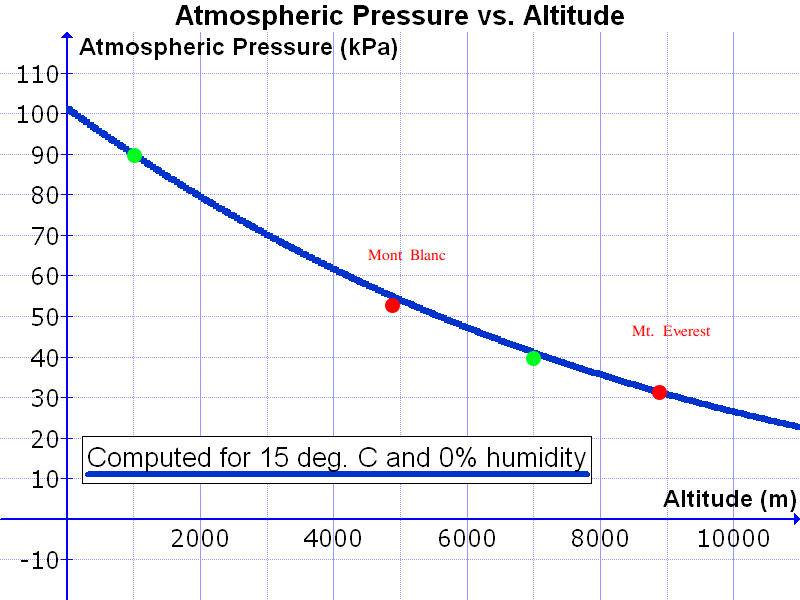
\includegraphics{Atmospheric_Pressure_vs._Altitude.png}
\caption{Atmospheric pressure versus altitude (wikipedia). Green points
represent our measurements, red points represent
interpolation/extrapolation.}
\end{figure}

    \hypertarget{discount-curve-interpolation}{%
\subsection{Discount curve
interpolation}\label{discount-curve-interpolation}}

Now we can come back to finance and using what we have just learnt try
to write a function which interpolates some given discount factors.

Needed data: * a list of pillars dates specifying the value dates of the
given discount factors, \(t_0,...,t_{n-1}\) * a list of given discount
factors, \(D(t_0),...,D(t_{n-1})\) * a pricing date (`today' date) which
corresponds to \(t=0\)

The input argument to the function will be the value date at which we
want to interpolate the discount factor.

Since the discount factor can be expresses as \(D=e^{-r(T-t)}\) the
function will use a log-linear interpolation to return the value we are
looking for.

\[D(t) = \mathrm{exp}\Big( (1-w)\cdot \mathrm{ln}(D(t_i)) + w\cdot \mathrm{ln}(D(t_{i+1}))\Big);\;\;\;w=\frac{t-t_i}{t_{i+1}-t_i}\]

where \(i\) is such that \(t_i \le t \le t_{i+1}\). More technically we
can say that we are doing a linear interpolation over time in the log
space:

\[d(t_i):=\mathrm{ln}(D(t_i))\]

\[d(t) = (1-w)d(t_i) + wd(t_{i+1});\;\;\;w=\frac{t-t_i}{t_{i+1}-t_i}\]

\[D(t) = \mathrm{exp}(d(t))\]

where \(i\) is such that \(t_i \le t \le t_{i+1}\)

Instead of reinventing the wheel and perform the interpolation with our
own code, we'll use the function \texttt{interp} provided by the Python
module \texttt{numpy}. So first let's try it with some simple examples:

    \begin{Verbatim}[commandchars=\\\{\}]
{\color{incolor}In [{\color{incolor}8}]:} \PY{c+c1}{\PYZsh{} let\PYZsq{}s assume we have a list \PYZsq{}xp\PYZsq{} of x-axis coordinates,}
        \PY{c+c1}{\PYZsh{} and the corresponding values \PYZsq{}fp\PYZsq{} of a function evaluated }
        \PY{c+c1}{\PYZsh{} at those x coordinates.}
        \PY{n}{xp} \PY{o}{=} \PY{p}{[}\PY{l+m+mi}{1}\PY{p}{,} \PY{l+m+mi}{2}\PY{p}{,} \PY{l+m+mi}{3}\PY{p}{]}
        \PY{n}{fp} \PY{o}{=} \PY{p}{[}\PY{l+m+mf}{0.3}\PY{p}{,} \PY{l+m+mf}{0.4}\PY{p}{,} \PY{l+m+mf}{0.6}\PY{p}{]}
        
        \PY{c+c1}{\PYZsh{} let\PYZsq{}s see what this looks like when plotted on a graph}
        \PY{c+c1}{\PYZsh{} we briefly introduce here the matplotlib module}
        \PY{c+c1}{\PYZsh{} the keyword as allows to give shorter names to modules}
        \PY{k+kn}{from} \PY{n+nn}{matplotlib} \PY{k}{import} \PY{n}{pyplot} \PY{k}{as} \PY{n}{plt}
        \PY{n}{plt}\PY{o}{.}\PY{n}{plot}\PY{p}{(}\PY{n}{xp}\PY{p}{,} \PY{n}{fp}\PY{p}{,} \PY{n}{marker}\PY{o}{=}\PY{l+s+s1}{\PYZsq{}}\PY{l+s+s1}{o}\PY{l+s+s1}{\PYZsq{}}\PY{p}{)}
        \PY{n}{plt}\PY{o}{.}\PY{n}{grid}\PY{p}{(}\PY{k+kc}{True}\PY{p}{)}
        \PY{n}{plt}\PY{o}{.}\PY{n}{show}\PY{p}{(}\PY{p}{)}
\end{Verbatim}

    \begin{center}
    \adjustimage{max size={0.9\linewidth}{0.9\paperheight}}{lecture_3_files/lecture_3_10_0.png}
    \end{center}
    { \hspace*{\fill} \\}
    
    \begin{Verbatim}[commandchars=\\\{\}]
{\color{incolor}In [{\color{incolor}9}]:} \PY{c+c1}{\PYZsh{} the numpy.interp function linearly interpolates these points to }
        \PY{c+c1}{\PYZsh{} estimate the value of f at other x coordinates. }
        \PY{c+c1}{\PYZsh{} For example, say we want to interpolate the points at x = 2.5::}
        \PY{k+kn}{import} \PY{n+nn}{numpy} \PY{k}{as} \PY{n+nn}{np}
        \PY{n}{np}\PY{o}{.}\PY{n}{interp}\PY{p}{(}\PY{l+m+mf}{2.5}\PY{p}{,} \PY{n}{xp}\PY{p}{,} \PY{n}{fp}\PY{p}{)}
\end{Verbatim}

\begin{Verbatim}[commandchars=\\\{\}]
{\color{outcolor}Out[{\color{outcolor}9}]:} 0.5
\end{Verbatim}
            
    \begin{Verbatim}[commandchars=\\\{\}]
{\color{incolor}In [{\color{incolor}10}]:} \PY{c+c1}{\PYZsh{} let\PYZsq{}s see what this looks like when plotted on a graph}
         
         \PY{k+kn}{from} \PY{n+nn}{matplotlib} \PY{k}{import} \PY{n}{pyplot} \PY{k}{as} \PY{n}{plt}
         \PY{n}{plt}\PY{o}{.}\PY{n}{plot}\PY{p}{(}\PY{n}{xp}\PY{p}{,} \PY{n}{fp}\PY{p}{,} \PY{n}{marker}\PY{o}{=}\PY{l+s+s1}{\PYZsq{}}\PY{l+s+s1}{o}\PY{l+s+s1}{\PYZsq{}}\PY{p}{)}
         \PY{n}{plt}\PY{o}{.}\PY{n}{grid}\PY{p}{(}\PY{k+kc}{True}\PY{p}{)}
         \PY{n}{plt}\PY{o}{.}\PY{n}{plot}\PY{p}{(}\PY{l+m+mf}{2.5}\PY{p}{,} \PY{n}{np}\PY{o}{.}\PY{n}{interp}\PY{p}{(}\PY{l+m+mf}{2.5}\PY{p}{,} \PY{n}{xp}\PY{p}{,} \PY{n}{fp}\PY{p}{)}\PY{p}{,} \PY{n}{marker}\PY{o}{=}\PY{l+s+s1}{\PYZsq{}}\PY{l+s+s1}{X}\PY{l+s+s1}{\PYZsq{}}\PY{p}{)}
         \PY{n}{plt}\PY{o}{.}\PY{n}{show}\PY{p}{(}\PY{p}{)}
\end{Verbatim}

    \begin{center}
    \adjustimage{max size={0.9\linewidth}{0.9\paperheight}}{lecture_3_files/lecture_3_12_0.png}
    \end{center}
    { \hspace*{\fill} \\}
    
    \hypertarget{interlude}{%
\subsubsection{Interlude}\label{interlude}}

How to learn about a given function ? Use the \texttt{help} keyword !

    \begin{Verbatim}[commandchars=\\\{\}]
{\color{incolor}In [{\color{incolor}11}]:} \PY{n}{help}\PY{p}{(}\PY{n}{np}\PY{o}{.}\PY{n}{interp}\PY{p}{)}
\end{Verbatim}

    \begin{Verbatim}[commandchars=\\\{\}]
Help on function interp in module numpy:

interp(x, xp, fp, left=None, right=None, period=None)
    One-dimensional linear interpolation.
    
    Returns the one-dimensional piecewise linear interpolant to a function
    with given discrete data points (`xp`, `fp`), evaluated at `x`.
    
    Parameters
    ----------
    x : array\_like
        The x-coordinates at which to evaluate the interpolated values.
    
    xp : 1-D sequence of floats
        The x-coordinates of the data points, must be increasing if argument
        `period` is not specified. Otherwise, `xp` is internally sorted after
        normalizing the periodic boundaries with ``xp = xp \% period``.
    
    fp : 1-D sequence of float or complex
        The y-coordinates of the data points, same length as `xp`.
    
    left : optional float or complex corresponding to fp
        Value to return for `x < xp[0]`, default is `fp[0]`.
    
    right : optional float or complex corresponding to fp
        Value to return for `x > xp[-1]`, default is `fp[-1]`.
    
    period : None or float, optional
        A period for the x-coordinates. This parameter allows the proper
        interpolation of angular x-coordinates. Parameters `left` and `right`
        are ignored if `period` is specified.
    
        .. versionadded:: 1.10.0
    
    Returns
    -------
    y : float or complex (corresponding to fp) or ndarray
        The interpolated values, same shape as `x`.
    
    Raises
    ------
    ValueError
        If `xp` and `fp` have different length
        If `xp` or `fp` are not 1-D sequences
        If `period == 0`
    
    Notes
    -----
    Does not check that the x-coordinate sequence `xp` is increasing.
    If `xp` is not increasing, the results are nonsense.
    A simple check for increasing is::
    
        np.all(np.diff(xp) > 0)
    
    Examples
    --------
    >>> xp = [1, 2, 3]
    >>> fp = [3, 2, 0]
    >>> np.interp(2.5, xp, fp)
    1.0
    >>> np.interp([0, 1, 1.5, 2.72, 3.14], xp, fp)
    array([ 3. ,  3. ,  2.5 ,  0.56,  0. ])
    >>> UNDEF = -99.0
    >>> np.interp(3.14, xp, fp, right=UNDEF)
    -99.0
    
    Plot an interpolant to the sine function:
    
    >>> x = np.linspace(0, 2*np.pi, 10)
    >>> y = np.sin(x)
    >>> xvals = np.linspace(0, 2*np.pi, 50)
    >>> yinterp = np.interp(xvals, x, y)
    >>> import matplotlib.pyplot as plt
    >>> plt.plot(x, y, 'o')
    [<matplotlib.lines.Line2D object at 0x{\ldots}>]
    >>> plt.plot(xvals, yinterp, '-x')
    [<matplotlib.lines.Line2D object at 0x{\ldots}>]
    >>> plt.show()
    
    Interpolation with periodic x-coordinates:
    
    >>> x = [-180, -170, -185, 185, -10, -5, 0, 365]
    >>> xp = [190, -190, 350, -350]
    >>> fp = [5, 10, 3, 4]
    >>> np.interp(x, xp, fp, period=360)
    array([7.5, 5., 8.75, 6.25, 3., 3.25, 3.5, 3.75])
    
    Complex interpolation:
    
    >>> x = [1.5, 4.0]
    >>> xp = [2,3,5]
    >>> fp = [1.0j, 0, 2+3j]
    >>> np.interp(x, xp, fp)
    array([ 0.+1.j ,  1.+1.5j])


    \end{Verbatim}

    \hypertarget{now-back-to-our-discount-factor-function-df.}{%
\subsubsection{Now back to our discount factor function
df.}\label{now-back-to-our-discount-factor-function-df.}}

    \begin{Verbatim}[commandchars=\\\{\}]
{\color{incolor}In [{\color{incolor}12}]:} \PY{c+c1}{\PYZsh{} import modules and objects that we need}
         \PY{k+kn}{from} \PY{n+nn}{datetime} \PY{k}{import} \PY{n}{date}
         \PY{k+kn}{import} \PY{n+nn}{numpy}\PY{o}{,} \PY{n+nn}{math}
         \PY{k+kn}{from} \PY{n+nn}{matplotlib} \PY{k}{import} \PY{n}{pyplot} \PY{k}{as} \PY{n}{plt}
         \PY{k+kn}{import} \PY{n+nn}{matplotlib}\PY{n+nn}{.}\PY{n+nn}{dates} \PY{k}{as} \PY{n+nn}{mdates} 
         \PY{c+c1}{\PYZsh{} with this notation we tell python to use mdates as an alias }
         \PY{c+c1}{\PYZsh{} for matplotlib.dates, I told you I\PYZsq{}m lazy...}
         
         \PY{c+c1}{\PYZsh{} define the input data}
         \PY{n}{today\PYZus{}date} \PY{o}{=} \PY{n}{date}\PY{p}{(}\PY{l+m+mi}{2019}\PY{p}{,} \PY{l+m+mi}{10}\PY{p}{,} \PY{l+m+mi}{1}\PY{p}{)}
         
         \PY{n}{pillar\PYZus{}dates} \PY{o}{=} \PY{p}{[}\PY{n}{date}\PY{p}{(}\PY{l+m+mi}{2019}\PY{p}{,} \PY{l+m+mi}{10}\PY{p}{,} \PY{l+m+mi}{1}\PY{p}{)}\PY{p}{,} \PY{n}{date}\PY{p}{(}\PY{l+m+mi}{2020}\PY{p}{,} \PY{l+m+mi}{10}\PY{p}{,} \PY{l+m+mi}{1}\PY{p}{)}\PY{p}{,} \PY{n}{date}\PY{p}{(}\PY{l+m+mi}{2021}\PY{p}{,} \PY{l+m+mi}{10}\PY{p}{,} \PY{l+m+mi}{1}\PY{p}{)}\PY{p}{]}
         \PY{n}{discount\PYZus{}factors} \PY{o}{=} \PY{p}{[}\PY{l+m+mf}{1.0}\PY{p}{,} \PY{l+m+mf}{0.97}\PY{p}{,} \PY{l+m+mf}{0.72}\PY{p}{]}
         
         \PY{c+c1}{\PYZsh{} let\PYZsq{}s see what this looks like when plotted on a graph}
         \PY{c+c1}{\PYZsh{} here a more complicated usage of matplotlib to}
         \PY{c+c1}{\PYZsh{} get a nicer plot}
         \PY{n}{plt}\PY{o}{.}\PY{n}{plot}\PY{p}{(}\PY{n}{pillar\PYZus{}dates}\PY{p}{,} \PY{n}{discount\PYZus{}factors}\PY{p}{,} \PY{n}{marker}\PY{o}{=}\PY{l+s+s1}{\PYZsq{}}\PY{l+s+s1}{o}\PY{l+s+s1}{\PYZsq{}}\PY{p}{)}
         \PY{n}{plt}\PY{o}{.}\PY{n}{gca}\PY{p}{(}\PY{p}{)}\PY{o}{.}\PY{n}{xaxis}\PY{o}{.}\PY{n}{set\PYZus{}major\PYZus{}formatter}\PY{p}{(}\PY{n}{mdates}\PY{o}{.}\PY{n}{DateFormatter}\PY{p}{(}\PY{l+s+s1}{\PYZsq{}}\PY{l+s+s1}{\PYZpc{}}\PY{l+s+s1}{m/}\PY{l+s+si}{\PYZpc{}d}\PY{l+s+s1}{/}\PY{l+s+s1}{\PYZpc{}}\PY{l+s+s1}{Y}\PY{l+s+s1}{\PYZsq{}}\PY{p}{)}\PY{p}{)}
         \PY{n}{plt}\PY{o}{.}\PY{n}{gca}\PY{p}{(}\PY{p}{)}\PY{o}{.}\PY{n}{xaxis}\PY{o}{.}\PY{n}{set\PYZus{}major\PYZus{}locator}\PY{p}{(}\PY{n}{mdates}\PY{o}{.}\PY{n}{YearLocator}\PY{p}{(}\PY{p}{)}\PY{p}{)}
         \PY{n}{plt}\PY{o}{.}\PY{n}{grid}\PY{p}{(}\PY{k+kc}{True}\PY{p}{)}
         \PY{n}{plt}\PY{o}{.}\PY{n}{show}\PY{p}{(}\PY{p}{)}
         
         \PY{c+c1}{\PYZsh{} define the df function}
         \PY{k}{def} \PY{n+nf}{df}\PY{p}{(}\PY{n}{d}\PY{p}{)}\PY{p}{:}
             \PY{c+c1}{\PYZsh{} first thing we need to do is to apply the logarithm function }
             \PY{c+c1}{\PYZsh{} to the discount factors since we are doing log-linear and}
             \PY{c+c1}{\PYZsh{} not just linear interpolation}
             \PY{n}{log\PYZus{}discount\PYZus{}factors} \PY{o}{=} \PY{p}{[}\PY{p}{]}
             \PY{k}{for} \PY{n}{discount\PYZus{}factor} \PY{o+ow}{in} \PY{n}{discount\PYZus{}factors}\PY{p}{:}
                 \PY{n}{log\PYZus{}discount\PYZus{}factors}\PY{o}{.}\PY{n}{append}\PY{p}{(}\PY{n}{math}\PY{o}{.}\PY{n}{log}\PY{p}{(}\PY{n}{discount\PYZus{}factor}\PY{p}{)}\PY{p}{)}
             
             \PY{c+c1}{\PYZsh{} perform the linear interpolation of the log discount factors}
             \PY{n}{interpolated\PYZus{}log\PYZus{}discount\PYZus{}factor} \PY{o}{=} \PYZbs{}
                 \PY{n}{numpy}\PY{o}{.}\PY{n}{interp}\PY{p}{(}\PY{n}{d}\PY{p}{,} \PY{n}{pillar\PYZus{}dates}\PY{p}{,} \PY{n}{log\PYZus{}discount\PYZus{}factors}\PY{p}{)}
             
             \PY{c+c1}{\PYZsh{} return the interpolated discount factor}
             \PY{k}{return} \PY{n}{math}\PY{o}{.}\PY{n}{exp}\PY{p}{(}\PY{n}{interpolated\PYZus{}log\PYZus{}discount\PYZus{}factor}\PY{p}{)}
\end{Verbatim}

    \begin{center}
    \adjustimage{max size={0.9\linewidth}{0.9\paperheight}}{lecture_3_files/lecture_3_16_0.png}
    \end{center}
    { \hspace*{\fill} \\}
    
    This is almost OK, \textbf{but it won't work} because
\texttt{numpy.interp} only accepts numbers/lists of numbers as arguments
i.e.~it doesn't automatically convert or interpret dates as numbers in
any way, so it doesn't know how to interpolate them. So we need to do
the conversion ourselves before passing the data into the
\texttt{numpy.interp} function.

    \begin{Verbatim}[commandchars=\\\{\}]
{\color{incolor}In [{\color{incolor}13}]:} \PY{k}{def} \PY{n+nf}{df}\PY{p}{(}\PY{n}{d}\PY{p}{)}\PY{p}{:}
             \PY{c+c1}{\PYZsh{} first thing we need to do is to apply the logarithm function}
             \PY{c+c1}{\PYZsh{} to the discount factors since we are doing log-linear and}
             \PY{c+c1}{\PYZsh{} not just linear interpolation}
             \PY{n}{log\PYZus{}discount\PYZus{}factors} \PY{o}{=} \PY{p}{[}\PY{p}{]}
             \PY{k}{for} \PY{n}{discount\PYZus{}factor} \PY{o+ow}{in} \PY{n}{discount\PYZus{}factors}\PY{p}{:}
                 \PY{n}{log\PYZus{}discount\PYZus{}factors}\PY{o}{.}\PY{n}{append}\PY{p}{(}\PY{n}{math}\PY{o}{.}\PY{n}{log}\PY{p}{(}\PY{n}{discount\PYZus{}factor}\PY{p}{)}\PY{p}{)}
             
             \PY{c+c1}{\PYZsh{} convert the pillar dates to pillar \PYZsq{}days\PYZsq{}}
             \PY{c+c1}{\PYZsh{} i.e. number of days from today}
             \PY{c+c1}{\PYZsh{} to write shorter code we can use this NEW notation}
             \PY{c+c1}{\PYZsh{} which condenses for and list creation in one line}
             \PY{n}{pillar\PYZus{}days} \PY{o}{=} \PYZbs{}
                 \PY{p}{[}\PY{p}{(}\PY{n}{pillar\PYZus{}date} \PY{o}{\PYZhy{}} \PY{n}{today\PYZus{}date}\PY{p}{)}\PY{o}{.}\PY{n}{days} \PY{k}{for} \PY{n}{pillar\PYZus{}date} \PY{o+ow}{in} \PY{n}{pillar\PYZus{}dates}\PY{p}{]}
             
             \PY{c+c1}{\PYZsh{} obviously we need to do the same to the value date}
             \PY{c+c1}{\PYZsh{} argument of the df function}
             \PY{n}{d\PYZus{}days} \PY{o}{=} \PY{p}{(}\PY{n}{d} \PY{o}{\PYZhy{}} \PY{n}{today\PYZus{}date}\PY{p}{)}\PY{o}{.}\PY{n}{days}
             
             \PY{c+c1}{\PYZsh{} perform the linear interpolation of the log discount factors}
             \PY{n}{interpolated\PYZus{}log\PYZus{}discount\PYZus{}factor} \PY{o}{=} \PYZbs{}
                 \PY{n}{numpy}\PY{o}{.}\PY{n}{interp}\PY{p}{(}\PY{n}{d\PYZus{}days}\PY{p}{,} \PY{n}{pillar\PYZus{}days}\PY{p}{,} \PY{n}{log\PYZus{}discount\PYZus{}factors}\PY{p}{)}
             
             \PY{c+c1}{\PYZsh{} return the interpolated discount factor}
             \PY{k}{return} \PY{n}{math}\PY{o}{.}\PY{n}{exp}\PY{p}{(}\PY{n}{interpolated\PYZus{}log\PYZus{}discount\PYZus{}factor}\PY{p}{)}
\end{Verbatim}

    \begin{Verbatim}[commandchars=\\\{\}]
{\color{incolor}In [{\color{incolor}18}]:} \PY{c+c1}{\PYZsh{} now we can use the df function to get discount factors}
         \PY{c+c1}{\PYZsh{} on value dates between the given pillar dates}
         \PY{n}{d0} \PY{o}{=} \PY{n}{date}\PY{p}{(}\PY{l+m+mi}{2020}\PY{p}{,} \PY{l+m+mi}{1}\PY{p}{,} \PY{l+m+mi}{1}\PY{p}{)}
         \PY{n}{df0} \PY{o}{=} \PY{n}{df}\PY{p}{(}\PY{n}{d0}\PY{p}{)}
         \PY{n+nb}{print} \PY{p}{(}\PY{n}{df0}\PY{p}{)}
\end{Verbatim}

    \begin{Verbatim}[commandchars=\\\{\}]
0.9923728228571693

    \end{Verbatim}

    \begin{Verbatim}[commandchars=\\\{\}]
{\color{incolor}In [{\color{incolor}15}]:} \PY{n}{d1} \PY{o}{=} \PY{n}{date}\PY{p}{(}\PY{l+m+mi}{2021}\PY{p}{,} \PY{l+m+mi}{1}\PY{p}{,} \PY{l+m+mi}{1}\PY{p}{)}
         \PY{n}{df1} \PY{o}{=} \PY{n}{df}\PY{p}{(}\PY{n}{d1}\PY{p}{)}
         \PY{n+nb}{print} \PY{p}{(}\PY{n}{df1}\PY{p}{)}
\end{Verbatim}

    \begin{Verbatim}[commandchars=\\\{\}]
0.8997999273630835

    \end{Verbatim}

    \begin{Verbatim}[commandchars=\\\{\}]
{\color{incolor}In [{\color{incolor}19}]:} \PY{c+c1}{\PYZsh{} let\PYZsq{}s see what these look like when plotted on a semi-log graph}
         
         \PY{k+kn}{from} \PY{n+nn}{matplotlib} \PY{k}{import} \PY{n}{pyplot} \PY{k}{as} \PY{n}{plt}
         \PY{k+kn}{import} \PY{n+nn}{matplotlib}\PY{n+nn}{.}\PY{n+nn}{dates} \PY{k}{as} \PY{n+nn}{mdates}
         \PY{n}{plt}\PY{o}{.}\PY{n}{semilogy}\PY{p}{(}\PY{n}{pillar\PYZus{}dates}\PY{p}{,} \PY{n}{discount\PYZus{}factors}\PY{p}{,} \PY{n}{marker}\PY{o}{=}\PY{l+s+s1}{\PYZsq{}}\PY{l+s+s1}{o}\PY{l+s+s1}{\PYZsq{}}\PY{p}{)}
         \PY{n}{plt}\PY{o}{.}\PY{n}{semilogy}\PY{p}{(}\PY{n}{d0}\PY{p}{,}\PY{n}{df0} \PY{p}{,} \PY{n}{marker}\PY{o}{=}\PY{l+s+s1}{\PYZsq{}}\PY{l+s+s1}{X}\PY{l+s+s1}{\PYZsq{}}\PY{p}{)}
         \PY{n}{plt}\PY{o}{.}\PY{n}{semilogy}\PY{p}{(}\PY{n}{d1}\PY{p}{,}\PY{n}{df1} \PY{p}{,} \PY{n}{marker}\PY{o}{=}\PY{l+s+s1}{\PYZsq{}}\PY{l+s+s1}{X}\PY{l+s+s1}{\PYZsq{}}\PY{p}{)}
         \PY{n}{plt}\PY{o}{.}\PY{n}{gca}\PY{p}{(}\PY{p}{)}\PY{o}{.}\PY{n}{xaxis}\PY{o}{.}\PY{n}{set\PYZus{}major\PYZus{}formatter}\PY{p}{(}\PY{n}{mdates}\PY{o}{.}\PY{n}{DateFormatter}\PY{p}{(}\PY{l+s+s1}{\PYZsq{}}\PY{l+s+s1}{\PYZpc{}}\PY{l+s+s1}{m/}\PY{l+s+si}{\PYZpc{}d}\PY{l+s+s1}{/}\PY{l+s+s1}{\PYZpc{}}\PY{l+s+s1}{Y}\PY{l+s+s1}{\PYZsq{}}\PY{p}{)}\PY{p}{)}
         \PY{n}{plt}\PY{o}{.}\PY{n}{gca}\PY{p}{(}\PY{p}{)}\PY{o}{.}\PY{n}{xaxis}\PY{o}{.}\PY{n}{set\PYZus{}major\PYZus{}locator}\PY{p}{(}\PY{n}{mdates}\PY{o}{.}\PY{n}{YearLocator}\PY{p}{(}\PY{p}{)}\PY{p}{)}
         \PY{n}{plt}\PY{o}{.}\PY{n}{grid}\PY{p}{(}\PY{k+kc}{True}\PY{p}{)}
         \PY{n}{plt}\PY{o}{.}\PY{n}{show}\PY{p}{(}\PY{p}{)}
\end{Verbatim}

    \begin{center}
    \adjustimage{max size={0.9\linewidth}{0.9\paperheight}}{lecture_3_files/lecture_3_21_0.png}
    \end{center}
    { \hspace*{\fill} \\}
    
    \begin{Verbatim}[commandchars=\\\{\}]
{\color{incolor}In [{\color{incolor}20}]:} \PY{c+c1}{\PYZsh{} let\PYZsq{}s see what these look like when plotted on a linear graph}
         
         \PY{k+kn}{from} \PY{n+nn}{matplotlib} \PY{k}{import} \PY{n}{pyplot} \PY{k}{as} \PY{n}{plt}
         \PY{k+kn}{import} \PY{n+nn}{matplotlib}\PY{n+nn}{.}\PY{n+nn}{dates} \PY{k}{as} \PY{n+nn}{mdates}
         \PY{n}{plt}\PY{o}{.}\PY{n}{plot}\PY{p}{(}\PY{n}{pillar\PYZus{}dates}\PY{p}{,} \PY{n}{discount\PYZus{}factors}\PY{p}{,} \PY{n}{marker}\PY{o}{=}\PY{l+s+s1}{\PYZsq{}}\PY{l+s+s1}{o}\PY{l+s+s1}{\PYZsq{}}\PY{p}{)}
         \PY{n}{plt}\PY{o}{.}\PY{n}{plot}\PY{p}{(}\PY{n}{d0}\PY{p}{,}\PY{n}{df0} \PY{p}{,} \PY{n}{marker}\PY{o}{=}\PY{l+s+s1}{\PYZsq{}}\PY{l+s+s1}{X}\PY{l+s+s1}{\PYZsq{}}\PY{p}{)}
         \PY{n}{plt}\PY{o}{.}\PY{n}{plot}\PY{p}{(}\PY{n}{d1}\PY{p}{,}\PY{n}{df1} \PY{p}{,} \PY{n}{marker}\PY{o}{=}\PY{l+s+s1}{\PYZsq{}}\PY{l+s+s1}{X}\PY{l+s+s1}{\PYZsq{}}\PY{p}{)}
         \PY{n}{plt}\PY{o}{.}\PY{n}{gca}\PY{p}{(}\PY{p}{)}\PY{o}{.}\PY{n}{xaxis}\PY{o}{.}\PY{n}{set\PYZus{}major\PYZus{}formatter}\PY{p}{(}\PY{n}{mdates}\PY{o}{.}\PY{n}{DateFormatter}\PY{p}{(}\PY{l+s+s1}{\PYZsq{}}\PY{l+s+s1}{\PYZpc{}}\PY{l+s+s1}{m/}\PY{l+s+si}{\PYZpc{}d}\PY{l+s+s1}{/}\PY{l+s+s1}{\PYZpc{}}\PY{l+s+s1}{Y}\PY{l+s+s1}{\PYZsq{}}\PY{p}{)}\PY{p}{)}
         \PY{n}{plt}\PY{o}{.}\PY{n}{gca}\PY{p}{(}\PY{p}{)}\PY{o}{.}\PY{n}{xaxis}\PY{o}{.}\PY{n}{set\PYZus{}major\PYZus{}locator}\PY{p}{(}\PY{n}{mdates}\PY{o}{.}\PY{n}{YearLocator}\PY{p}{(}\PY{p}{)}\PY{p}{)}
         \PY{n}{plt}\PY{o}{.}\PY{n}{grid}\PY{p}{(}\PY{k+kc}{True}\PY{p}{)}
         \PY{n}{plt}\PY{o}{.}\PY{n}{show}\PY{p}{(}\PY{p}{)}
\end{Verbatim}

    \begin{center}
    \adjustimage{max size={0.9\linewidth}{0.9\paperheight}}{lecture_3_files/lecture_3_22_0.png}
    \end{center}
    { \hspace*{\fill} \\}
    
    \hypertarget{exercises}{%
\subsection{Exercises}\label{exercises}}

\hypertarget{exercise-3.1}{%
\subsubsection{Exercise 3.1}\label{exercise-3.1}}

Take the code for the Black-Scholes formula from Exercise 2.3 and wrap
it in a function. Then, use this function to calculate the prices of
calls with various strikes, using the following data.

\begin{Shaded}
\begin{Highlighting}[]
\NormalTok{S_t }\OperatorTok{=} \DecValTok{800}
\CommentTok{# strikes expressed as % of spot price}
\NormalTok{moneyness }\OperatorTok{=}\NormalTok{ [ }\FloatTok{0.5}\NormalTok{, }\FloatTok{0.75}\NormalTok{, }\FloatTok{0.825}\NormalTok{, }\FloatTok{1.0}\NormalTok{, }\FloatTok{1.125}\NormalTok{, }\FloatTok{1.25}\NormalTok{, }\FloatTok{1.5}\NormalTok{ ]   }
\NormalTok{vol }\OperatorTok{=} \FloatTok{0.3}
\NormalTok{ttm }\OperatorTok{=} \FloatTok{0.75}
\NormalTok{r }\OperatorTok{=} \FloatTok{0.005}
\end{Highlighting}
\end{Shaded}

The output should be a dictionary mapping strikes to call prices.

\hypertarget{exercise-3.2}{%
\subsubsection{Exercise 3.2}\label{exercise-3.2}}

Python has a useful command called \texttt{assert} which can be used for
checking that a given condition is satisfied, and raising an error if
the condition is not satisfied.

The following line does not cause an error, in fact it does nothing

\begin{Shaded}
\begin{Highlighting}[]
\ControlFlowTok{assert} \DecValTok{1} \OperatorTok{<} \DecValTok{2}
\end{Highlighting}
\end{Shaded}

This causes an error

\begin{Shaded}
\begin{Highlighting}[]
\ControlFlowTok{assert} \DecValTok{1} \OperatorTok{>} \DecValTok{2}
\end{Highlighting}
\end{Shaded}

\texttt{assert} can take a second parameter with a message to display in case of failure:

\begin{Shaded}
\begin{Highlighting}[]
\ControlFlowTok{assert} \DecValTok{1} \OperatorTok{>} \DecValTok{2}, ``Two is bigger than one''
\end{Highlighting}
\end{Shaded}

Take the \texttt{df} function from this lesson and modify it by adding some
assertions to check that:
\begin{itemize}
\item the pillar date list contains at least 2 elements
\item the pillar date list is the same length as the discount factor list
\item the first pillar date is equal to the today date
\item the value date argument 'd' is greater or equal to the first pillar date and also less than or equal to the last pillar date
\end{itemize}

Then try using the function with some invalid data to make sure that
your assertions are correctly checking the desired conditions.

\hypertarget{exercise-3.3}{%
\subsubsection{Exercise 3.3}\label{exercise-3.3}}

Python has a module called \texttt{matplotlib} which can be used for
plotting graphs and charts. In particular, we can use a sub-module
called \texttt{pyplot} which provides slightly easier-to-use interface
for plotting interactively.

\begin{Shaded}
\begin{Highlighting}[]
\ImportTok{from}\NormalTok{ matplotlib }\ImportTok{import}\NormalTok{ pyplot}

\CommentTok{# plot some data}
\NormalTok{pyplot.plot(}
\NormalTok{    [}\DecValTok{1}\NormalTok{, }\DecValTok{2}\NormalTok{, }\DecValTok{3}\NormalTok{],   }\CommentTok{# x-axis coordinates}
\NormalTok{    [}\DecValTok{5}\NormalTok{, }\DecValTok{3}\NormalTok{, }\DecValTok{10}\NormalTok{],  }\CommentTok{# y-axis coordinates}
\NormalTok{    marker}\OperatorTok{=}\StringTok{'o'}   \CommentTok{# we want the points to be marked with circles}
\NormalTok{)}
\end{Highlighting}
\end{Shaded}

Use this function to plot the call prices from exercise 3.1. Remember to
use \texttt{help} and \texttt{dir} to have some help (or to look in
Google ;-)).

    \hypertarget{advanced-hint}{%
\subsection{Advanced hint}\label{advanced-hint}}

Interpolation using \texttt{scipy.interpolate}:
https://docs.scipy.org/doc/scipy-0.15.1/reference/interpolate.html\#module-scipy.interpolate


    % Add a bibliography block to the postdoc
    
    
    
    \end{document}

\clearpage

% Default to the notebook output style

    


% Inherit from the specified cell style.




    
\documentclass[11pt]{article}

    
    
    \usepackage[T1]{fontenc}
    % Nicer default font (+ math font) than Computer Modern for most use cases
    \usepackage{mathpazo}

    % Basic figure setup, for now with no caption control since it's done
    % automatically by Pandoc (which extracts ![](path) syntax from Markdown).
    \usepackage{graphicx}
    % We will generate all images so they have a width \maxwidth. This means
    % that they will get their normal width if they fit onto the page, but
    % are scaled down if they would overflow the margins.
    \makeatletter
    \def\maxwidth{\ifdim\Gin@nat@width>\linewidth\linewidth
    \else\Gin@nat@width\fi}
    \makeatother
    \let\Oldincludegraphics\includegraphics
    % Set max figure width to be 80% of text width, for now hardcoded.
    \renewcommand{\includegraphics}[1]{\Oldincludegraphics[width=.8\maxwidth]{#1}}
    % Ensure that by default, figures have no caption (until we provide a
    % proper Figure object with a Caption API and a way to capture that
    % in the conversion process - todo).
    \usepackage{caption}
    \DeclareCaptionLabelFormat{nolabel}{}
    \captionsetup{labelformat=nolabel}

    \usepackage{adjustbox} % Used to constrain images to a maximum size 
    \usepackage{xcolor} % Allow colors to be defined
    \usepackage{enumerate} % Needed for markdown enumerations to work
    \usepackage{geometry} % Used to adjust the document margins
    \usepackage{amsmath} % Equations
    \usepackage{amssymb} % Equations
    \usepackage{textcomp} % defines textquotesingle
    % Hack from http://tex.stackexchange.com/a/47451/13684:
    \AtBeginDocument{%
        \def\PYZsq{\textquotesingle}% Upright quotes in Pygmentized code
    }
    \usepackage{upquote} % Upright quotes for verbatim code
    \usepackage{eurosym} % defines \euro
    \usepackage[mathletters]{ucs} % Extended unicode (utf-8) support
    \usepackage[utf8x]{inputenc} % Allow utf-8 characters in the tex document
    \usepackage{fancyvrb} % verbatim replacement that allows latex
    \usepackage{grffile} % extends the file name processing of package graphics 
                         % to support a larger range 
    % The hyperref package gives us a pdf with properly built
    % internal navigation ('pdf bookmarks' for the table of contents,
    % internal cross-reference links, web links for URLs, etc.)
    \usepackage{hyperref}
    \usepackage{longtable} % longtable support required by pandoc >1.10
    \usepackage{booktabs}  % table support for pandoc > 1.12.2
    \usepackage[inline]{enumitem} % IRkernel/repr support (it uses the enumerate* environment)
    \usepackage[normalem]{ulem} % ulem is needed to support strikethroughs (\sout)
                                % normalem makes italics be italics, not underlines
    \usepackage{mathrsfs}
    

    
    
    % Colors for the hyperref package
    \definecolor{urlcolor}{rgb}{0,.145,.698}
    \definecolor{linkcolor}{rgb}{.71,0.21,0.01}
    \definecolor{citecolor}{rgb}{.12,.54,.11}

    % ANSI colors
    \definecolor{ansi-black}{HTML}{3E424D}
    \definecolor{ansi-black-intense}{HTML}{282C36}
    \definecolor{ansi-red}{HTML}{E75C58}
    \definecolor{ansi-red-intense}{HTML}{B22B31}
    \definecolor{ansi-green}{HTML}{00A250}
    \definecolor{ansi-green-intense}{HTML}{007427}
    \definecolor{ansi-yellow}{HTML}{DDB62B}
    \definecolor{ansi-yellow-intense}{HTML}{B27D12}
    \definecolor{ansi-blue}{HTML}{208FFB}
    \definecolor{ansi-blue-intense}{HTML}{0065CA}
    \definecolor{ansi-magenta}{HTML}{D160C4}
    \definecolor{ansi-magenta-intense}{HTML}{A03196}
    \definecolor{ansi-cyan}{HTML}{60C6C8}
    \definecolor{ansi-cyan-intense}{HTML}{258F8F}
    \definecolor{ansi-white}{HTML}{C5C1B4}
    \definecolor{ansi-white-intense}{HTML}{A1A6B2}
    \definecolor{ansi-default-inverse-fg}{HTML}{FFFFFF}
    \definecolor{ansi-default-inverse-bg}{HTML}{000000}

    % commands and environments needed by pandoc snippets
    % extracted from the output of `pandoc -s`
    \providecommand{\tightlist}{%
      \setlength{\itemsep}{0pt}\setlength{\parskip}{0pt}}
    \DefineVerbatimEnvironment{Highlighting}{Verbatim}{commandchars=\\\{\}}
    % Add ',fontsize=\small' for more characters per line
    \newenvironment{Shaded}{}{}
    \newcommand{\KeywordTok}[1]{\textcolor[rgb]{0.00,0.44,0.13}{\textbf{{#1}}}}
    \newcommand{\DataTypeTok}[1]{\textcolor[rgb]{0.56,0.13,0.00}{{#1}}}
    \newcommand{\DecValTok}[1]{\textcolor[rgb]{0.25,0.63,0.44}{{#1}}}
    \newcommand{\BaseNTok}[1]{\textcolor[rgb]{0.25,0.63,0.44}{{#1}}}
    \newcommand{\FloatTok}[1]{\textcolor[rgb]{0.25,0.63,0.44}{{#1}}}
    \newcommand{\CharTok}[1]{\textcolor[rgb]{0.25,0.44,0.63}{{#1}}}
    \newcommand{\StringTok}[1]{\textcolor[rgb]{0.25,0.44,0.63}{{#1}}}
    \newcommand{\CommentTok}[1]{\textcolor[rgb]{0.38,0.63,0.69}{\textit{{#1}}}}
    \newcommand{\OtherTok}[1]{\textcolor[rgb]{0.00,0.44,0.13}{{#1}}}
    \newcommand{\AlertTok}[1]{\textcolor[rgb]{1.00,0.00,0.00}{\textbf{{#1}}}}
    \newcommand{\FunctionTok}[1]{\textcolor[rgb]{0.02,0.16,0.49}{{#1}}}
    \newcommand{\RegionMarkerTok}[1]{{#1}}
    \newcommand{\ErrorTok}[1]{\textcolor[rgb]{1.00,0.00,0.00}{\textbf{{#1}}}}
    \newcommand{\NormalTok}[1]{{#1}}
    
    % Additional commands for more recent versions of Pandoc
    \newcommand{\ConstantTok}[1]{\textcolor[rgb]{0.53,0.00,0.00}{{#1}}}
    \newcommand{\SpecialCharTok}[1]{\textcolor[rgb]{0.25,0.44,0.63}{{#1}}}
    \newcommand{\VerbatimStringTok}[1]{\textcolor[rgb]{0.25,0.44,0.63}{{#1}}}
    \newcommand{\SpecialStringTok}[1]{\textcolor[rgb]{0.73,0.40,0.53}{{#1}}}
    \newcommand{\ImportTok}[1]{{#1}}
    \newcommand{\DocumentationTok}[1]{\textcolor[rgb]{0.73,0.13,0.13}{\textit{{#1}}}}
    \newcommand{\AnnotationTok}[1]{\textcolor[rgb]{0.38,0.63,0.69}{\textbf{\textit{{#1}}}}}
    \newcommand{\CommentVarTok}[1]{\textcolor[rgb]{0.38,0.63,0.69}{\textbf{\textit{{#1}}}}}
    \newcommand{\VariableTok}[1]{\textcolor[rgb]{0.10,0.09,0.49}{{#1}}}
    \newcommand{\ControlFlowTok}[1]{\textcolor[rgb]{0.00,0.44,0.13}{\textbf{{#1}}}}
    \newcommand{\OperatorTok}[1]{\textcolor[rgb]{0.40,0.40,0.40}{{#1}}}
    \newcommand{\BuiltInTok}[1]{{#1}}
    \newcommand{\ExtensionTok}[1]{{#1}}
    \newcommand{\PreprocessorTok}[1]{\textcolor[rgb]{0.74,0.48,0.00}{{#1}}}
    \newcommand{\AttributeTok}[1]{\textcolor[rgb]{0.49,0.56,0.16}{{#1}}}
    \newcommand{\InformationTok}[1]{\textcolor[rgb]{0.38,0.63,0.69}{\textbf{\textit{{#1}}}}}
    \newcommand{\WarningTok}[1]{\textcolor[rgb]{0.38,0.63,0.69}{\textbf{\textit{{#1}}}}}
    
    
    % Define a nice break command that doesn't care if a line doesn't already
    % exist.
    \def\br{\hspace*{\fill} \\* }
    % Math Jax compatibility definitions
    \def\gt{>}
    \def\lt{<}
    \let\Oldtex\TeX
    \let\Oldlatex\LaTeX
    \renewcommand{\TeX}{\textrm{\Oldtex}}
    \renewcommand{\LaTeX}{\textrm{\Oldlatex}}
    % Document parameters
    % Document title
    \title{Swaps and Modules - Practical Lesson 5}
    \author{Matteo Sani \\ \href{mailto:matteosan1@gmail.com}{matteosan1@gmail.com}}
    
    
    
    

    % Pygments definitions
    
\makeatletter
\def\PY@reset{\let\PY@it=\relax \let\PY@bf=\relax%
    \let\PY@ul=\relax \let\PY@tc=\relax%
    \let\PY@bc=\relax \let\PY@ff=\relax}
\def\PY@tok#1{\csname PY@tok@#1\endcsname}
\def\PY@toks#1+{\ifx\relax#1\empty\else%
    \PY@tok{#1}\expandafter\PY@toks\fi}
\def\PY@do#1{\PY@bc{\PY@tc{\PY@ul{%
    \PY@it{\PY@bf{\PY@ff{#1}}}}}}}
\def\PY#1#2{\PY@reset\PY@toks#1+\relax+\PY@do{#2}}

\expandafter\def\csname PY@tok@w\endcsname{\def\PY@tc##1{\textcolor[rgb]{0.73,0.73,0.73}{##1}}}
\expandafter\def\csname PY@tok@c\endcsname{\let\PY@it=\textit\def\PY@tc##1{\textcolor[rgb]{0.25,0.50,0.50}{##1}}}
\expandafter\def\csname PY@tok@cp\endcsname{\def\PY@tc##1{\textcolor[rgb]{0.74,0.48,0.00}{##1}}}
\expandafter\def\csname PY@tok@k\endcsname{\let\PY@bf=\textbf\def\PY@tc##1{\textcolor[rgb]{0.00,0.50,0.00}{##1}}}
\expandafter\def\csname PY@tok@kp\endcsname{\def\PY@tc##1{\textcolor[rgb]{0.00,0.50,0.00}{##1}}}
\expandafter\def\csname PY@tok@kt\endcsname{\def\PY@tc##1{\textcolor[rgb]{0.69,0.00,0.25}{##1}}}
\expandafter\def\csname PY@tok@o\endcsname{\def\PY@tc##1{\textcolor[rgb]{0.40,0.40,0.40}{##1}}}
\expandafter\def\csname PY@tok@ow\endcsname{\let\PY@bf=\textbf\def\PY@tc##1{\textcolor[rgb]{0.67,0.13,1.00}{##1}}}
\expandafter\def\csname PY@tok@nb\endcsname{\def\PY@tc##1{\textcolor[rgb]{0.00,0.50,0.00}{##1}}}
\expandafter\def\csname PY@tok@nf\endcsname{\def\PY@tc##1{\textcolor[rgb]{0.00,0.00,1.00}{##1}}}
\expandafter\def\csname PY@tok@nc\endcsname{\let\PY@bf=\textbf\def\PY@tc##1{\textcolor[rgb]{0.00,0.00,1.00}{##1}}}
\expandafter\def\csname PY@tok@nn\endcsname{\let\PY@bf=\textbf\def\PY@tc##1{\textcolor[rgb]{0.00,0.00,1.00}{##1}}}
\expandafter\def\csname PY@tok@ne\endcsname{\let\PY@bf=\textbf\def\PY@tc##1{\textcolor[rgb]{0.82,0.25,0.23}{##1}}}
\expandafter\def\csname PY@tok@nv\endcsname{\def\PY@tc##1{\textcolor[rgb]{0.10,0.09,0.49}{##1}}}
\expandafter\def\csname PY@tok@no\endcsname{\def\PY@tc##1{\textcolor[rgb]{0.53,0.00,0.00}{##1}}}
\expandafter\def\csname PY@tok@nl\endcsname{\def\PY@tc##1{\textcolor[rgb]{0.63,0.63,0.00}{##1}}}
\expandafter\def\csname PY@tok@ni\endcsname{\let\PY@bf=\textbf\def\PY@tc##1{\textcolor[rgb]{0.60,0.60,0.60}{##1}}}
\expandafter\def\csname PY@tok@na\endcsname{\def\PY@tc##1{\textcolor[rgb]{0.49,0.56,0.16}{##1}}}
\expandafter\def\csname PY@tok@nt\endcsname{\let\PY@bf=\textbf\def\PY@tc##1{\textcolor[rgb]{0.00,0.50,0.00}{##1}}}
\expandafter\def\csname PY@tok@nd\endcsname{\def\PY@tc##1{\textcolor[rgb]{0.67,0.13,1.00}{##1}}}
\expandafter\def\csname PY@tok@s\endcsname{\def\PY@tc##1{\textcolor[rgb]{0.73,0.13,0.13}{##1}}}
\expandafter\def\csname PY@tok@sd\endcsname{\let\PY@it=\textit\def\PY@tc##1{\textcolor[rgb]{0.73,0.13,0.13}{##1}}}
\expandafter\def\csname PY@tok@si\endcsname{\let\PY@bf=\textbf\def\PY@tc##1{\textcolor[rgb]{0.73,0.40,0.53}{##1}}}
\expandafter\def\csname PY@tok@se\endcsname{\let\PY@bf=\textbf\def\PY@tc##1{\textcolor[rgb]{0.73,0.40,0.13}{##1}}}
\expandafter\def\csname PY@tok@sr\endcsname{\def\PY@tc##1{\textcolor[rgb]{0.73,0.40,0.53}{##1}}}
\expandafter\def\csname PY@tok@ss\endcsname{\def\PY@tc##1{\textcolor[rgb]{0.10,0.09,0.49}{##1}}}
\expandafter\def\csname PY@tok@sx\endcsname{\def\PY@tc##1{\textcolor[rgb]{0.00,0.50,0.00}{##1}}}
\expandafter\def\csname PY@tok@m\endcsname{\def\PY@tc##1{\textcolor[rgb]{0.40,0.40,0.40}{##1}}}
\expandafter\def\csname PY@tok@gh\endcsname{\let\PY@bf=\textbf\def\PY@tc##1{\textcolor[rgb]{0.00,0.00,0.50}{##1}}}
\expandafter\def\csname PY@tok@gu\endcsname{\let\PY@bf=\textbf\def\PY@tc##1{\textcolor[rgb]{0.50,0.00,0.50}{##1}}}
\expandafter\def\csname PY@tok@gd\endcsname{\def\PY@tc##1{\textcolor[rgb]{0.63,0.00,0.00}{##1}}}
\expandafter\def\csname PY@tok@gi\endcsname{\def\PY@tc##1{\textcolor[rgb]{0.00,0.63,0.00}{##1}}}
\expandafter\def\csname PY@tok@gr\endcsname{\def\PY@tc##1{\textcolor[rgb]{1.00,0.00,0.00}{##1}}}
\expandafter\def\csname PY@tok@ge\endcsname{\let\PY@it=\textit}
\expandafter\def\csname PY@tok@gs\endcsname{\let\PY@bf=\textbf}
\expandafter\def\csname PY@tok@gp\endcsname{\let\PY@bf=\textbf\def\PY@tc##1{\textcolor[rgb]{0.00,0.00,0.50}{##1}}}
\expandafter\def\csname PY@tok@go\endcsname{\def\PY@tc##1{\textcolor[rgb]{0.53,0.53,0.53}{##1}}}
\expandafter\def\csname PY@tok@gt\endcsname{\def\PY@tc##1{\textcolor[rgb]{0.00,0.27,0.87}{##1}}}
\expandafter\def\csname PY@tok@err\endcsname{\def\PY@bc##1{\setlength{\fboxsep}{0pt}\fcolorbox[rgb]{1.00,0.00,0.00}{1,1,1}{\strut ##1}}}
\expandafter\def\csname PY@tok@kc\endcsname{\let\PY@bf=\textbf\def\PY@tc##1{\textcolor[rgb]{0.00,0.50,0.00}{##1}}}
\expandafter\def\csname PY@tok@kd\endcsname{\let\PY@bf=\textbf\def\PY@tc##1{\textcolor[rgb]{0.00,0.50,0.00}{##1}}}
\expandafter\def\csname PY@tok@kn\endcsname{\let\PY@bf=\textbf\def\PY@tc##1{\textcolor[rgb]{0.00,0.50,0.00}{##1}}}
\expandafter\def\csname PY@tok@kr\endcsname{\let\PY@bf=\textbf\def\PY@tc##1{\textcolor[rgb]{0.00,0.50,0.00}{##1}}}
\expandafter\def\csname PY@tok@bp\endcsname{\def\PY@tc##1{\textcolor[rgb]{0.00,0.50,0.00}{##1}}}
\expandafter\def\csname PY@tok@fm\endcsname{\def\PY@tc##1{\textcolor[rgb]{0.00,0.00,1.00}{##1}}}
\expandafter\def\csname PY@tok@vc\endcsname{\def\PY@tc##1{\textcolor[rgb]{0.10,0.09,0.49}{##1}}}
\expandafter\def\csname PY@tok@vg\endcsname{\def\PY@tc##1{\textcolor[rgb]{0.10,0.09,0.49}{##1}}}
\expandafter\def\csname PY@tok@vi\endcsname{\def\PY@tc##1{\textcolor[rgb]{0.10,0.09,0.49}{##1}}}
\expandafter\def\csname PY@tok@vm\endcsname{\def\PY@tc##1{\textcolor[rgb]{0.10,0.09,0.49}{##1}}}
\expandafter\def\csname PY@tok@sa\endcsname{\def\PY@tc##1{\textcolor[rgb]{0.73,0.13,0.13}{##1}}}
\expandafter\def\csname PY@tok@sb\endcsname{\def\PY@tc##1{\textcolor[rgb]{0.73,0.13,0.13}{##1}}}
\expandafter\def\csname PY@tok@sc\endcsname{\def\PY@tc##1{\textcolor[rgb]{0.73,0.13,0.13}{##1}}}
\expandafter\def\csname PY@tok@dl\endcsname{\def\PY@tc##1{\textcolor[rgb]{0.73,0.13,0.13}{##1}}}
\expandafter\def\csname PY@tok@s2\endcsname{\def\PY@tc##1{\textcolor[rgb]{0.73,0.13,0.13}{##1}}}
\expandafter\def\csname PY@tok@sh\endcsname{\def\PY@tc##1{\textcolor[rgb]{0.73,0.13,0.13}{##1}}}
\expandafter\def\csname PY@tok@s1\endcsname{\def\PY@tc##1{\textcolor[rgb]{0.73,0.13,0.13}{##1}}}
\expandafter\def\csname PY@tok@mb\endcsname{\def\PY@tc##1{\textcolor[rgb]{0.40,0.40,0.40}{##1}}}
\expandafter\def\csname PY@tok@mf\endcsname{\def\PY@tc##1{\textcolor[rgb]{0.40,0.40,0.40}{##1}}}
\expandafter\def\csname PY@tok@mh\endcsname{\def\PY@tc##1{\textcolor[rgb]{0.40,0.40,0.40}{##1}}}
\expandafter\def\csname PY@tok@mi\endcsname{\def\PY@tc##1{\textcolor[rgb]{0.40,0.40,0.40}{##1}}}
\expandafter\def\csname PY@tok@il\endcsname{\def\PY@tc##1{\textcolor[rgb]{0.40,0.40,0.40}{##1}}}
\expandafter\def\csname PY@tok@mo\endcsname{\def\PY@tc##1{\textcolor[rgb]{0.40,0.40,0.40}{##1}}}
\expandafter\def\csname PY@tok@ch\endcsname{\let\PY@it=\textit\def\PY@tc##1{\textcolor[rgb]{0.25,0.50,0.50}{##1}}}
\expandafter\def\csname PY@tok@cm\endcsname{\let\PY@it=\textit\def\PY@tc##1{\textcolor[rgb]{0.25,0.50,0.50}{##1}}}
\expandafter\def\csname PY@tok@cpf\endcsname{\let\PY@it=\textit\def\PY@tc##1{\textcolor[rgb]{0.25,0.50,0.50}{##1}}}
\expandafter\def\csname PY@tok@c1\endcsname{\let\PY@it=\textit\def\PY@tc##1{\textcolor[rgb]{0.25,0.50,0.50}{##1}}}
\expandafter\def\csname PY@tok@cs\endcsname{\let\PY@it=\textit\def\PY@tc##1{\textcolor[rgb]{0.25,0.50,0.50}{##1}}}

\def\PYZbs{\char`\\}
\def\PYZus{\char`\_}
\def\PYZob{\char`\{}
\def\PYZcb{\char`\}}
\def\PYZca{\char`\^}
\def\PYZam{\char`\&}
\def\PYZlt{\char`\<}
\def\PYZgt{\char`\>}
\def\PYZsh{\char`\#}
\def\PYZpc{\char`\%}
\def\PYZdl{\char`\$}
\def\PYZhy{\char`\-}
\def\PYZsq{\char`\'}
\def\PYZdq{\char`\"}
\def\PYZti{\char`\~}
% for compatibility with earlier versions
\def\PYZat{@}
\def\PYZlb{[}
\def\PYZrb{]}
\makeatother


    % Exact colors from NB
    \definecolor{incolor}{rgb}{0.0, 0.0, 0.5}
    \definecolor{outcolor}{rgb}{0.545, 0.0, 0.0}



    
    % Prevent overflowing lines due to hard-to-break entities
    \sloppy 
    % Setup hyperref package
    \hypersetup{
      breaklinks=true,  % so long urls are correctly broken across lines
      colorlinks=true,
      urlcolor=urlcolor,
      linkcolor=linkcolor,
      citecolor=citecolor,
      }
    % Slightly bigger margins than the latex defaults
    
    \geometry{verbose,tmargin=1in,bmargin=1in,lmargin=1in,rmargin=1in}
    
    

    \begin{document}
    
    
    \maketitle
    
    

    
    \hypertarget{swaps-and-modules---practical-lesson-5}{%
\section{Swaps and Modules}\label{swaps-and-modules---practical-lesson-5}}

\hypertarget{recap}{%
\subsection{Recap}\label{recap}}

\begin{itemize}
\tightlist
\item
  basic Python (mostly not related directly to finance)
\item
  how to implement a discount factor interpolation function
\item
  qrapping up functionality in classes in order to work with multiple
  data sets more easily
\item
  libor forward rate calculator
\end{itemize}

\hypertarget{todays-lesson}{%
\subsection{Today's lesson}\label{todays-lesson}}

We're going to look at: * modules, and start building up our library of
finance-related functionality * implementing an Overnight Index Swap
class for calculating the NPV of an OIS.

\hypertarget{modules}{%
\section{Modules}\label{modules}}

An interactive session (e.g notebook or interactive shell) is great for
quick testing and exploratory use, but once you have some code
(i.e.~functions or classes) which you'd like to reuse often, rather than
copy/pasting it every time you need it, you can save it in a .py file
and use it from your session (aka you can create your own library).

These work just like the modules we have been importing up to now,
except they're written by us! Take a look at this video
(https://www.youtube.com/watch?v=AqCl65wxikw) for an example of how it's
done for Jupyter notebook.

We're going to start writing a module called \textbf{finmarkets}, and
over the course of the remaining lessons we'll add functionality related
to the theory lessons.

So first of all let's create a new file called finmarkets.py and copy
into it the \texttt{DiscountCurve} class we wrote last time.

    \begin{Verbatim}[commandchars=\\\{\}]
{\color{incolor}In [{\color{incolor}1}]:} \PY{k+kn}{from} \PY{n+nn}{datetime} \PY{k}{import} \PY{n}{date}
        \PY{k+kn}{from} \PY{n+nn}{finmarkets} \PY{k}{import} \PY{n}{DiscountCurve}
        
        \PY{n}{curve} \PY{o}{=} \PY{n}{DiscountCurve}\PY{p}{(}\PY{n}{date}\PY{p}{(}\PY{l+m+mi}{2019}\PY{p}{,} \PY{l+m+mi}{1}\PY{p}{,} \PY{l+m+mi}{1}\PY{p}{)}\PY{p}{,}
                              \PY{p}{[}\PY{n}{date}\PY{p}{(}\PY{l+m+mi}{2019}\PY{p}{,} \PY{l+m+mi}{1}\PY{p}{,} \PY{l+m+mi}{1}\PY{p}{)}\PY{p}{,} 
                               \PY{n}{date}\PY{p}{(}\PY{l+m+mi}{2019}\PY{p}{,} \PY{l+m+mi}{6}\PY{p}{,} \PY{l+m+mi}{1}\PY{p}{)}\PY{p}{,} 
                               \PY{n}{date}\PY{p}{(}\PY{l+m+mi}{2020}\PY{p}{,} \PY{l+m+mi}{1}\PY{p}{,} \PY{l+m+mi}{1}\PY{p}{)}\PY{p}{]}\PY{p}{,}
                              \PY{p}{[}\PY{l+m+mf}{1.0}\PY{p}{,} \PY{l+m+mf}{0.98}\PY{p}{,} \PY{l+m+mf}{0.82}\PY{p}{]}\PY{p}{)}
        \PY{n}{curve}\PY{o}{.}\PY{n}{df}\PY{p}{(}\PY{n}{date}\PY{p}{(}\PY{l+m+mi}{2019}\PY{p}{,} \PY{l+m+mi}{7}\PY{p}{,} \PY{l+m+mi}{1}\PY{p}{)}\PY{p}{)}
\end{Verbatim}

\begin{Verbatim}[commandchars=\\\{\}]
{\color{outcolor}Out[{\color{outcolor}1}]:} 0.9558151167629666
\end{Verbatim}
            
    We will use this discount curve later in this lesson.

\hypertarget{overnight-index-swap}{%
\section{Overnight Index Swap}\label{overnight-index-swap}}

Overnight Index Swap (OIS) are products which pay a floating coupon,
determined by overnight rate fixings over the reference periods, against
a fixed coupon. We will always look at these products from the point of
view of the \textbf{receiver of the floating leg}. Therefore an OIS is
defined by:

\begin{itemize}
\tightlist
\item
  a notional amount \(N\)
\item
  a start date \(d_0\)
\item
  a sequence of payment dates \(d_1,...,d_n\)
\item
  a fixed rate \(K\)
\end{itemize}

For simplicity we're assuming that the fixed and floating legs have the
same notional and payment dates, although this is not necessarily always
the case in practice.

At each payment date, the floating leg pays a cash flow determined as
follows:

\[f_{\mathrm{float},~i} = N \Bigg\{\prod_{d=d_{i-1}}^{d=d_i-1}\Big(1+r_{o/n}(d)\cdot\frac{1}{360}\Big) -1 \Bigg\}\]

(This formula is valid for an EONIA swap, i.e.~for OIS swaps in EUR,
other currencies might have different conventions. The \(\frac{1}{360}\)
fraction appears because EONIA rates are quoted using the ACT/360
daycount convention and here we're making a simplifying assumption of
ignoring weekends and holidays, so we assume that each overnight rate is
valid for only one day.)

The sum of the discounted expected values of these cashflows is

\[\mathrm{NPV}_{\mathrm{float}} = \sum_{i=1}^{n}D(d_i)\mathbb{E}[f_{\mathrm{float},~i}]\]

where \(D(d)\) is the discount factor with expiry \(d\). On the other
hand, by definition (remember practical lesson 4 with forward rates), we
also have the following relationship

\[\mathbb{E}[f_{\mathrm{float},~i}] = N\cdot\Big(\frac{D_{ois}(d_{i-1})}{D_{ois}(d_{i})} - 1\Big) \]

where \(D_{ois}(d)\) is the discount factor implied by OIS prices.

In a previous theory lesson we mentioned that the correct curve to use
for discounting the flows of a collateralized contract is the one
associated with the collateral. Since OIS contracts are collateralized
with cash, and cash accrues daily interes at the overnight rate, the OIS
curve is itself the correct curve with which to discount the flows of an
OIS contract !

In summary, \(D = D_{ois}\) so the NPV simplifies to

\[\mathrm{NPV}_{\mathrm{float}} = N\cdot\sum_{i=1}^{n}[D(d_{i-1}) - D(d_i)] = N \cdot [D(d_0) - D(d_n)]\]

Each cash flow of the fixed leg is equal to

\[f_{\mathrm{fix},~i}=N\cdot K\cdot \frac{d_i - d_{i-1}}{360}\]

so the NPV of the fixed leg is

\[\mathrm{NPV}_{\mathrm{fix}} = N\cdot K\cdot \sum_{i=1}^{n}D(d_{i})\frac{d_i - d_{i-1}}{360}\]

Ultimately the aim will be to take a series of OIS quotations, and
determine the discount factors implied by their prices. To do this we'll
build a pricing function (or rather a class), which takes discount curve
as the input and produces the net present value (NPV) of the OIS as the
output. Next lesson we'll put this function inside a numerical optimizer
to invert the process and hence to determine the implied discount
factors from the prices.

    \begin{Verbatim}[commandchars=\\\{\}]
{\color{incolor}In [{\color{incolor}2}]:} \PY{k}{class} \PY{n+nc}{OvernightIndexSwap}\PY{p}{(}\PY{n+nb}{object}\PY{p}{)}\PY{p}{:}
        
            \PY{c+c1}{\PYZsh{} this method is called to build the instance,}
            \PY{c+c1}{\PYZsh{} we take some data arguments and save them as}
            \PY{c+c1}{\PYZsh{} attributes of self }
            \PY{c+c1}{\PYZsh{} n.b.: payment\PYZus{}dates should be a list of dates,}
            \PY{c+c1}{\PYZsh{} including the start date as the first element}
            \PY{k}{def} \PY{n+nf}{\PYZus{}\PYZus{}init\PYZus{}\PYZus{}}\PY{p}{(}\PY{n+nb+bp}{self}\PY{p}{,} \PY{n}{notional}\PY{p}{,} \PY{n}{payment\PYZus{}dates}\PY{p}{,} \PY{n}{fixed\PYZus{}rate}\PY{p}{)}\PY{p}{:}
                \PY{n+nb+bp}{self}\PY{o}{.}\PY{n}{notional} \PY{o}{=} \PY{n}{notional}
                \PY{n+nb+bp}{self}\PY{o}{.}\PY{n}{payment\PYZus{}dates} \PY{o}{=} \PY{n}{payment\PYZus{}dates}
                \PY{n+nb+bp}{self}\PY{o}{.}\PY{n}{fixed\PYZus{}rate} \PY{o}{=} \PY{n}{fixed\PYZus{}rate}
                
            \PY{c+c1}{\PYZsh{} this method takes a discount curve and calculates}
            \PY{c+c1}{\PYZsh{} the NPV of the floating leg using that curve}
            \PY{k}{def} \PY{n+nf}{npv\PYZus{}floating\PYZus{}leg}\PY{p}{(}\PY{n+nb+bp}{self}\PY{p}{,} \PY{n}{discount\PYZus{}curve}\PY{p}{)}\PY{p}{:}
                \PY{c+c1}{\PYZsh{} self.payment\PYZus{}date s[0] is the start date of the swap}
                \PY{c+c1}{\PYZsh{} self.payment\PYZus{}date s[-1] is the last payment date of the swap}
                \PY{k}{return} \PY{n+nb+bp}{self}\PY{o}{.}\PY{n}{notional} \PY{o}{*} \PY{p}{(}\PY{n}{discount\PYZus{}curve}\PY{o}{.}\PY{n}{df}\PY{p}{(}\PY{n+nb+bp}{self}\PY{o}{.}\PY{n}{payment\PYZus{}dates}\PY{p}{[}\PY{l+m+mi}{0}\PY{p}{]}\PY{p}{)} \PY{o}{\PYZhy{}} 
                                        \PY{n}{discount\PYZus{}curve}\PY{o}{.}\PY{n}{df}\PY{p}{(}\PY{n+nb+bp}{self}\PY{o}{.}\PY{n}{payment\PYZus{}dates}\PY{p}{[}\PY{o}{\PYZhy{}}\PY{l+m+mi}{1}\PY{p}{]}\PY{p}{)}\PY{p}{)}
            
            \PY{c+c1}{\PYZsh{} this method takes a discount curve and calculates the NPV}
            \PY{c+c1}{\PYZsh{} of the fixed leg using that curve}
            \PY{k}{def} \PY{n+nf}{npv\PYZus{}fixed\PYZus{}leg}\PY{p}{(}\PY{n+nb+bp}{self}\PY{p}{,} \PY{n}{discount\PYZus{}curve}\PY{p}{)}\PY{p}{:}
                \PY{n}{npv} \PY{o}{=} \PY{l+m+mi}{0}
                \PY{c+c1}{\PYZsh{} we loop from i=1 up to but not including the length of the date list}
                \PY{k}{for} \PY{n}{i} \PY{o+ow}{in} \PY{n+nb}{range}\PY{p}{(}\PY{l+m+mi}{1}\PY{p}{,} \PY{n+nb}{len}\PY{p}{(}\PY{n+nb+bp}{self}\PY{o}{.}\PY{n}{payment\PYZus{}dates}\PY{p}{)}\PY{p}{)}\PY{p}{:} 
                    \PY{c+c1}{\PYZsh{} we can do i-1, because the loop starts with i=1}
                    \PY{n}{start\PYZus{}date} \PY{o}{=} \PY{n+nb+bp}{self}\PY{o}{.}\PY{n}{payment\PYZus{}dates}\PY{p}{[}\PY{n}{i}\PY{o}{\PYZhy{}}\PY{l+m+mi}{1}\PY{p}{]} 
                    \PY{n}{end\PYZus{}date} \PY{o}{=} \PY{n+nb+bp}{self}\PY{o}{.}\PY{n}{payment\PYZus{}dates}\PY{p}{[}\PY{n}{i}\PY{p}{]}
                    \PY{n}{tau} \PY{o}{=} \PY{p}{(}\PY{n}{end\PYZus{}date} \PY{o}{\PYZhy{}} \PY{n}{start\PYZus{}date}\PY{p}{)}\PY{o}{.}\PY{n}{days} \PY{o}{/} \PY{l+m+mi}{360}
                    \PY{n}{df} \PY{o}{=} \PY{n}{discount\PYZus{}curve}\PY{o}{.}\PY{n}{df}\PY{p}{(}\PY{n}{end\PYZus{}date}\PY{p}{)}
                    \PY{n}{npv} \PY{o}{=} \PY{n}{npv} \PY{o}{+} \PY{n}{df} \PY{o}{*} \PY{n}{tau}
                    \PY{k}{return} \PY{n+nb+bp}{self}\PY{o}{.}\PY{n}{notional} \PY{o}{*} \PY{n+nb+bp}{self}\PY{o}{.}\PY{n}{fixed\PYZus{}rate} \PY{o}{*} \PY{n}{npv}
            
            \PY{c+c1}{\PYZsh{} this method calculates the NPV of the OIS swap}
            \PY{c+c1}{\PYZsh{} n.b.: inside this method we call the other two }
            \PY{c+c1}{\PYZsh{} methods of the class on the same instance \PYZsq{}self\PYZsq{},}
            \PY{c+c1}{\PYZsh{} using self.npv\PYZus{}XXX\PYZus{}leg(...), and we pass the }
            \PY{c+c1}{\PYZsh{} discount\PYZus{}curve we received as an argument}
            \PY{k}{def} \PY{n+nf}{npv}\PY{p}{(}\PY{n+nb+bp}{self}\PY{p}{,} \PY{n}{discount\PYZus{}curve}\PY{p}{)}\PY{p}{:}
                \PY{n}{float\PYZus{}npv} \PY{o}{=} \PY{n+nb+bp}{self}\PY{o}{.}\PY{n}{npv\PYZus{}floating\PYZus{}leg}\PY{p}{(}\PY{n}{discount\PYZus{}curve}\PY{p}{)}
                \PY{n}{fixed\PYZus{}npv} \PY{o}{=} \PY{n+nb+bp}{self}\PY{o}{.}\PY{n}{npv\PYZus{}fixed\PYZus{}leg}\PY{p}{(}\PY{n}{discount\PYZus{}curve}\PY{p}{)}
                \PY{k}{return} \PY{n}{float\PYZus{}npv} \PY{o}{\PYZhy{}} \PY{n}{fixed\PYZus{}npv}
\end{Verbatim}

    \begin{Verbatim}[commandchars=\\\{\}]
{\color{incolor}In [{\color{incolor}3}]:} \PY{k+kn}{from} \PY{n+nn}{datetime} \PY{k}{import} \PY{n}{date}
        
        \PY{n}{ois} \PY{o}{=} \PY{n}{OvernightIndexSwap}\PY{p}{(}
            \PY{c+c1}{\PYZsh{} the notional, one million}
            \PY{l+m+mf}{1e6}\PY{p}{,}
            \PY{c+c1}{\PYZsh{} the list of product dates, }
            \PY{c+c1}{\PYZsh{} i.e. the start date then the payment dates}
            \PY{p}{[}\PY{n}{date}\PY{p}{(}\PY{l+m+mi}{2019}\PY{p}{,} \PY{l+m+mi}{1}\PY{p}{,} \PY{l+m+mi}{1}\PY{p}{)}\PY{p}{,} 
             \PY{n}{date}\PY{p}{(}\PY{l+m+mi}{2019}\PY{p}{,} \PY{l+m+mi}{4}\PY{p}{,} \PY{l+m+mi}{1}\PY{p}{)}\PY{p}{,} 
             \PY{n}{date}\PY{p}{(}\PY{l+m+mi}{2019}\PY{p}{,} \PY{l+m+mi}{7}\PY{p}{,} \PY{l+m+mi}{1}\PY{p}{)}\PY{p}{,} 
             \PY{n}{date}\PY{p}{(}\PY{l+m+mi}{2019}\PY{p}{,} \PY{l+m+mi}{10}\PY{p}{,} \PY{l+m+mi}{1}\PY{p}{)}\PY{p}{,}
             \PY{n}{date}\PY{p}{(}\PY{l+m+mi}{2020}\PY{p}{,} \PY{l+m+mi}{1}\PY{p}{,} \PY{l+m+mi}{1}\PY{p}{)}\PY{p}{]}\PY{p}{,}
            \PY{c+c1}{\PYZsh{} the fixed rate, 2.5\PYZpc{}}
            \PY{l+m+mf}{0.025}
        \PY{p}{)}
\end{Verbatim}

    We can now use the curve we have prepared at the beginning of the lesson
and that we stored in a variable called curve. Let's now evaluate the
NPV of the OIS.

    \begin{Verbatim}[commandchars=\\\{\}]
{\color{incolor}In [{\color{incolor}4}]:} \PY{n}{ois}\PY{o}{.}\PY{n}{npv}\PY{p}{(}\PY{n}{curve}\PY{p}{)}
\end{Verbatim}

\begin{Verbatim}[commandchars=\\\{\}]
{\color{outcolor}Out[{\color{outcolor}4}]:} 173824.80713628858
\end{Verbatim}
            
    \hypertarget{exercises}{%
\subsection{Exercises}\label{exercises}}

\hypertarget{exercise-5.1}{%
\subsubsection{Exercise 5.1}\label{exercise-5.1}}

Take the \texttt{OvernightIndexSwap} class from the lesson and add a new
method called fair\_value\_strike which takes a discount curve object
and returns the fixed rate which would make the OIS have zero NPV.

\emph{Hints}: * first take the formulas for the NPV of the fixed leg and
the NPV of the floating leg, put one equal to the other and solve for
\(K\); * then implement that in Python.

\hypertarget{exercise-5.2}{%
\subsubsection{Exercise 5.2}\label{exercise-5.2}}

Take the \texttt{OvernightIndexSwap} class, add it to
\texttt{finmarkets.py} and try importing and using it.

\hypertarget{exercise-5.3}{%
\subsubsection{Exercise 5.3}\label{exercise-5.3}}

In the next lesson we're going to build lots of
\texttt{OvernightIndexSwap} objects, one for each market quote we have.
The market quotes will consist of fixed strikes for 1M, 2M, 3M,
\ldots{}, 12M, 15M, 18M, 2Y, 3Y, \ldots{}, 30Y and 40Y swaps.

It would be very boring to write a long list of payment dates for each
one of these, plus they'd need to be updated every day. Write a function
which given a start date and the number of months, returns a list of
dates of \textbf{annual} frequency starting from the start date and
ending after the specified number of months.

For example

2016-11-17 start date 12 months \(\rightarrow\) 2016-11-17, 2017-11-17
2016-11-17 start date 24 months \(\rightarrow\) 2016-11-17, 2017-11-17,
2018-11-17

Note that if the number of months is not a multiple of 12, the last
period should simply be shorter than 12 months. For example

2016-11-17 start date 9 months \(\rightarrow\) 2016-11-17, 2017-08-17
2016-11-17 start date 15 months \(\rightarrow\) 2016-11-17, 2017-11-17,
2018-02-17

Here's some skeleton code to help you get started:

\begin{Shaded}
\begin{Highlighting}[]
\ImportTok{from}\NormalTok{ dateutil }\ImportTok{import}\NormalTok{ relativedelta}

\KeywordTok{def}\NormalTok{ generate_swap_dates(start_date, n_months):}
\NormalTok{    dates }\OperatorTok{=}\NormalTok{ []}
    \CommentTok{# your code here which adds all the relevant dates to the dates list}
    \ControlFlowTok{return}\NormalTok{ dates}
\end{Highlighting}
\end{Shaded}

\begin{Shaded}
\begin{Highlighting}[]
\CommentTok{# some tests to check if the function is working correctly}
\ImportTok{from}\NormalTok{ datetime }\ImportTok{import}\NormalTok{ date}

\ControlFlowTok{assert}\NormalTok{ generate_swap_dates(date(}\DecValTok{2016}\NormalTok{, }\DecValTok{11}\NormalTok{, }\DecValTok{17}\NormalTok{), }\DecValTok{12}\NormalTok{) }\OperatorTok{==}\NormalTok{ [date(}\DecValTok{2016}\NormalTok{, }\DecValTok{11}\NormalTok{, }\DecValTok{17}\NormalTok{), }
\NormalTok{                                                       date(}\DecValTok{2017}\NormalTok{, }\DecValTok{11}\NormalTok{, }\DecValTok{17}\NormalTok{)]}
\ControlFlowTok{assert}\NormalTok{ generate_swap_dates(date(}\DecValTok{2016}\NormalTok{, }\DecValTok{11}\NormalTok{, }\DecValTok{17}\NormalTok{), }\DecValTok{24}\NormalTok{) }\OperatorTok{==}\NormalTok{ [date(}\DecValTok{2016}\NormalTok{, }\DecValTok{11}\NormalTok{, }\DecValTok{17}\NormalTok{), }
\NormalTok{                                                       date(}\DecValTok{2017}\NormalTok{, }\DecValTok{11}\NormalTok{, }\DecValTok{17}\NormalTok{), }
\NormalTok{                                                       date(}\DecValTok{2018}\NormalTok{, }\DecValTok{11}\NormalTok{, }\DecValTok{17}\NormalTok{)]}

\ControlFlowTok{assert}\NormalTok{ generate_swap_dates(date(}\DecValTok{2016}\NormalTok{, }\DecValTok{11}\NormalTok{, }\DecValTok{17}\NormalTok{), }\DecValTok{9}\NormalTok{) }\OperatorTok{==}\NormalTok{ [date(}\DecValTok{2016}\NormalTok{, }\DecValTok{11}\NormalTok{, }\DecValTok{17}\NormalTok{), }
\NormalTok{                                                      date(}\DecValTok{2017}\NormalTok{, }\DecValTok{8}\NormalTok{, }\DecValTok{17}\NormalTok{)]}
\ControlFlowTok{assert}\NormalTok{ generate_swap_dates(date(}\DecValTok{2016}\NormalTok{, }\DecValTok{11}\NormalTok{, }\DecValTok{17}\NormalTok{), }\DecValTok{15}\NormalTok{) }\OperatorTok{==}\NormalTok{ [date(}\DecValTok{2016}\NormalTok{, }\DecValTok{11}\NormalTok{, }\DecValTok{17}\NormalTok{), }
\NormalTok{                                                       date(}\DecValTok{2017}\NormalTok{, }\DecValTok{11}\NormalTok{, }\DecValTok{17}\NormalTok{), }
\NormalTok{                                                       date(}\DecValTok{2018}\NormalTok{, }\DecValTok{2}\NormalTok{, }\DecValTok{17}\NormalTok{)]}
\end{Highlighting}
\end{Shaded}


    % Add a bibliography block to the postdoc
    
    
    
    \end{document}

\clearpage

\end{document}
